\documentclass[Dual]{iitm-thesis}

\usepackage[font=small]{caption}
\usepackage{palatino}
\usepackage{framed}
\usepackage{mdframed}

\usepackage{graphicx}
\usepackage{hyperref} % hyperlinks for references.
\hypersetup{ 
  pdftitle          = {Improving the performance of dynamic critiquing},
  pdfauthor         = {Bharath Reddy <bharath270392@gmail.com>},
}
\usepackage{amsmath} % easier math formulae, align, subequations \ldots
\usepackage{amsfonts}   
\usepackage{amssymb}   
\usepackage{amsthm}   

\usepackage{longtable}% for long tables
\usepackage{booktabs} % Table rules
\usepackage{subfig} 
\usepackage[ruled,vlined,linesnumbered]{algorithm2e} 

\usepackage{tikz} 
\usepackage{varwidth}
\usepackage{algpseudocode}

\usepackage{fancyvrb}
\usepackage{multicol}
\usepackage{multirow}
\usepackage{mathtools}
\usepackage{lipsum}



% Section References
\newcommand{\secref}[1] {\hyperref[#1]{Section~\ref*{#1}}}
\newcommand{\sectionref}[1] {\hyperref[#1]{Section~\ref*{#1}}}
\newcommand{\chapterref}[1] {\hyperref[#1]{Chapter~\ref*{#1}}}
\newcommand{\appendixref}[1] {\hyperref[#1]{Appendix~\ref*{#1}}}
\newcommand{\exref}[1] {\hyperref[#1]{Example~\ref*{#1}}}

\newcommand{\eqnref}[1] {Equation \eqref{#1}}
\newcommand{\draft}[1] {{\bf TODO: #1}}

\newcommand{\figref}[1] {\hyperref[#1]{Figure~\ref*{#1}}}
\newcommand{\algoref}[1] {\hyperref[#1]{Algorithm~\ref*{#1}}}
\newcommand{\thmref}[1] {\hyperref[#1]{Theorem~\ref*{#1}}}
\newcommand{\lmref}[1] {\hyperref[#1]{Lemma~\ref*{#1}}}
%\renewcommand{\algorithmiccomment}[1]{\textit{// #1}}

\theoremstyle{plain} 
\newtheorem{example}{Example}
\newtheorem{theorem}{Theorem}
\newtheorem{lemma}[theorem]{Lemma}
\newtheorem{proposition}[theorem]{Proposition}
\newtheorem{remark}[theorem]{Remark}
\newtheorem{corollary}[theorem]{Corollary}
\newtheorem{definition}[theorem]{Definition}
\newtheorem{conjecture}[theorem]{Conjecture}
\newtheorem{axiom}[theorem]{Axiom}
\newtheorem{note}{Note}
\newtheorem{property}{Property}


%Math Operators
\DeclareMathOperator {\argmax} {argmax}
\DeclareMathOperator {\argmin} {argmin}
\DeclareMathOperator {\sgn} {sgn}
\DeclareMathOperator {\Tr} {tr}
\DeclareMathOperator{\E} {\mathbb{E}}
\DeclareMathOperator{\Var} {Var}

\newcommand{\ud}{\, \mathrm{d}}
\newcommand{\diff}[1] {\frac{\partial}{\, \partial #1}}
\newcommand{\diffn}[2] {\frac{\partial^{#2}}{\, \partial {#1}^{#2}}}
\newcommand{\grad} {\nabla}
\newcommand{\tuple}[1] {\langle #1 \rangle}
\newcommand{\innerprod}[2] {\langle #1, #2 \rangle}

% Constants/etc.
\renewcommand{\Re} {\mathbb{R}}
\newcommand{\Cm} {\mathbb{C}}
\newcommand{\Qm} {\mathbb{Q}}
\newcommand{\half} {\frac{1}{2}}
\newcommand{\finv}[1] {{#1}^{-1}}

\newcommand{\states} {S}
\newcommand{\States} {\mathcal{S}}
\newcommand{\transitions} {P}
\newcommand{\Transitions} {\mathcal{P}}
\newcommand{\Observations} {\Omega}
\newcommand{\Obs} {\Omega}
\newcommand{\emissions} {O}
\newcommand{\actions} {A}
\newcommand{\Actions} {\mathcal{A}}
\newcommand{\rewards} {R}
\newcommand{\Rewards} {\mathcal{R}}
\newcommand{\graph} {\mathcal{G}}
\newcommand{\mdp} {M}
\newcommand{\Mdp} {\mathcal{M}}
\newcommand{\policy} {\pi}
\newcommand{\initset} {\mathcal{I}}
\newcommand{\stopcond} {\beta}
\newcommand{\option} {\tuple{ \initset,\policy,\stopcond} }
\newcommand{\options} {\mathcal{O}}

%
\DeclareMathOperator {\measure} {\mathcal{X}}

%Math Operators
\DeclareMathOperator {\Qf} {Q}
\DeclareMathOperator {\Vf} {V}

% Homs
\newcommand{\him}[1] {\ensuremath{\underline{#1}}}
\renewcommand{\hom}[1] {\xrightarrow{#1}}
\newcommand{\homset} {\mathcal{H}}


\newcommand{\GProc} {\mathcal{GP}}
\newcommand{\mL} {\mathcal{L}}

%Math Operators
\DeclareMathOperator {\ball} {B}
\DeclareMathOperator {\ballf} {B^{f}}
\DeclareMathOperator {\sball} {b}
\DeclareMathOperator {\sballf} {b^{f}}

%Short hand
\newcommand{\arbcnst} {\tilde{c}}
\newcommand{\greedyalgo} {\ensuremath{\mathcal{GA}~}}
\newcommand{\egreedyalgo} {\ensuremath{\mathcal{GA}_{\epsilon}~}}
\newcommand{\epsilonm} {\bar{\epsilon}}

\newcommand{\klein} {\mathcal{K}}



\newcommand{\mytitle}{Improving the performance of Dynamic Critiquing}
\newcommand{\myauthor}{Bharath Reddy A}

\title{\mytitle}
\author{\myauthor}
\date{April 2014}
\department{COMPUTER SCIENCE AND ENGINEERING}

\begin{document}

% Title page
%\nocite{*}
\maketitle

%uncomment the next 8 lines when report is done..
% Certificate
%% Certificate
\certificate

\vspace*{0.5in}

\noindent This is to certify that the thesis titled {\bf \mytitle}
submitted by {\bf \myauthor}, to the Indian Institute of Technology,
Madras, for the award of the degrees of {\bf Bachelor of Technology and
Master of Technology}, is a bona fide record of the research work done
by him under our supervision.  The contents of this thesis, in full or
in parts, have not been submitted to any other Institute or University
for the award of any degree or diploma.

\vspace*{1.5in}

\begin{singlespacing}
\hspace*{-0.25in}
\parbox{2.5in}{
\noindent {\bf Dr. Sutanu Chakraborti} \\
\noindent Assistant Professor \\
\noindent Dept. of Computer Science and Engineering\\
\noindent IIT-Madras, 600 036 \\
} 
\hspace*{1.0in} 
%\parbox{2.5in}{
%\noindent {\bf Prof.~S.~C.~Rajan} \\
%\noindent Research Guide \\ 
%\noindent Assistant Professor \\
%\noindent Dept.  of  Aerospace Engineering\\
%\noindent IIT-Madras, 600 036 \\
%}  
\end{singlespacing}

\vspace*{0.25in}
\noindent Place: Chennai\\
\noindent Date: 



% Acknowledgements
%\acknowledgements
$<TODO>$

%I am very thankful to Dr. Sutanu Chakraborti <fill-TODO>
%
%I am grateful to my friends Skanda Raj, Shubranshu Shekar, Saurabh Gupta and Dileep for helping me a lot during the project.
%
%I thank the Department of Computer Science as
%whole. 
%I have got such a good experience during the last 5 years. For this, the credit must go to remarkable
%teachers like  Dr. Madhu Mutyam, Dr. Shankar Balachandran, Dr.
%Sutanu Chakraborti, Dr. Ravindran and Dr. C Pandu Rangan
%


% Abstract
%\abstract
\vspace*{24pt}

Most commercial recommender systems in practice use collaborative filtering (CF) techniques that rely heavily on user-ratings to make recommendations. 
However, CF techniques may not perform well in high-risk product domains like cars, cameras, houses etc. where there a low number of ratings.Knowledge based Recommenders are used to provide recommendations in these scenarios.
In these domains, users often want to define their requirements explicitly - "The maximum price of the computer should be \$1400 and Hard-drive capacity should be atleast 500 GB." and engage in an interaction with the system.
Knowledge based(KB) recommender systems are used to generate appropriate recommendations in these scenarios.
Knowledge based systems mimic the kind of dialog that takes place between a customer and shopkeeper involving multiple interactions and where the user can give feedback at every interaction.
\textit{Critiquing} is a popular form of feedback in conversational recommendation systems.

Dynamic generation of appropriate compound critiques in each cycle is a critical issue for critique-based conversational recommender systems.
In earlier research, Apriori algorithm and Multi Attribute Utility Theory (MAUT) based generation of compound critiques have been proposed.
MAUT based recommendation has been shown to be slightly superior to Apriori Algorithm based recommendation in offline experiments and live user studies.
The average number of interaction cycles per recommendation session is a measure that is often used to measure the efficiency of a recommendation algorithm. 
Lower the number of cycles, better is the performance of the algorithm. 
In this project, we propose several modifications to the MAUT based generation of compound critiques and report the performance improvements caused by each of these modifications.






%Furthermore, a user's taste for products in these domains keeps changing with time. For example, if a user gave a rating of 5 stars to a Pentium-II computer 6 years ago, using that rating in making new recommendations will be in-appropriate.


\pagebreak

% Table of contents etc.
% Uncomment these lines when this report is done...
%\begin{singlespace}
%\tableofcontents
%\thispagestyle{empty}
%\listoftables
%\addcontentsline{toc}{chapter}{LIST OF TABLES}
%\listoffigures
%\addcontentsline{toc}{chapter}{LIST OF FIGURES}
%\end{singlespace}

% Abbreviations
%\abbreviations

\noindent 
\begin{tabbing}
xxxxxxxxxxx \= xxxxxxxxxxxxxxxxxxxxxxxxxxxxxxxxxxxxxxxxxxxxxxxx \kill
\textbf{IITM}   \> Indian Institute of Technology, Madras \\
\textbf{RTFM} \> Read the Fine Manual \\
\end{tabbing}

\pagebreak
%\chapter*{\centerline{NOTATION}}
\addcontentsline{toc}{chapter}{NOTATION}

\begin{singlespace}
\begin{tabbing}
xxxxxxxxxxx \= xxxxxxxxxxxxxxxxxxxxxxxxxxxxxxxxxxxxxxxxxxxxxxxx \kill
\textbf{$r$}  \> Radius, $m$ \\
\textbf{$\alpha$}  \> Angle of thesis in degrees \\
\textbf{$\beta$}   \> Flight path in degrees \\
\end{tabbing}
\end{singlespace}

%\pagebreak
\clearpage

% The main text will follow from this point so set the page numbering
% to arabic from here on.
\pagenumbering{arabic}

% Chapters-old
%\chapter{Introduction}
\label{chap:intro}

% High level introduction about the kinda learning we are talking
% about
Reinforcement learning (RL) is a widely studied learning framework for
autonomous agents, particularly because of it's extreme generality; it
addresses the problem of learning optimal agent behaviour in an
unknown stochastic environment. In this setting, an agent explores
a state space, receiving rewards for actions it takes; the objective
of the agent is to maximise it's rewards accumulated over time. In the
conventional setting, the agent approaches each new problem from
scratch. We would like to study how the agent can exploit solutions it
has already learnt in order to solve a new task.

\section{Exploiting Structure}

% Types of structure - temporal abstractions - options
To reuse behavioural policies, we need to either identify some
`structure' in the environment or to impose such `structure' ourselves
to transfer the policy. This structure is roughly identified through
spatial and temporal abstractions. One approach for the former is to
form a hierarchical representation of the environment, creating
a factored MDP \citep{Guestrin2003}. Yet another, one that we adopt in
this work, is to identify correspondences, or homomorphisms, between
states either in the same environment (i.e.  a ``symmetry''), or between
environments. There exist several criteria for these correspondences;
\citet{Li2006} present a survey of various approaches taken in the
community, and relate them to each other.

With temporal abstractions, high-level actions are introduced which
capture sequences of primitive actions. In this light, temporal
abstractions capture the notion of a ``subtask''. The most common
approach for temporal abstractions is the options framework proposed by
\citet{SuttonPrecupSingh1999}; we adopt this framework as well.
\citet{Ravindran2003} show how temporal abstractions can be combined
with spatial abstractions using relativised options. Both spatial and
temporal abstractions play an important role in transfer learning, where
we wish to extend optimal behaviour learnt in one task to another task.
These approaches fall under the broader field of transfer learning;
a survey of many other transfer learning techniques can be found in
\citet{Taylor2009a}.

\subsection{A Motivating Example: Controlling an Octopus Arm}
% Describe roughly the kind of figures we're seeing with the octopus
% example

\begin{figure}[ht]
  \centering
  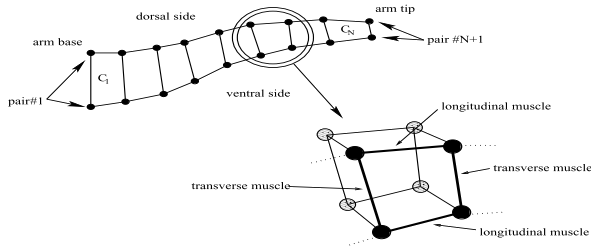
\includegraphics[width=5in]{figures/octopus-arm} 
  \caption{Dynamics of an Octopus Arm}
  \label{fig:octopus-arm}
\end{figure}

As a motivating example for abstraction, consider the control of an
octopus arm, as shown in \figref{fig:octopus-arm}. This arm can be
modelled as a composition of 10 compartments, each of which can be
controlled by contracting longitudinal and transverse muscles
\citep{Engel2006}. In total, there are 88 continuous state variables
associated with the arm, and it is controlled with a 32 dimensional,
continuous valued signal. A typical task in such a domain is to move
the arm to grab at a particular location, somewhere in space. The
space may include obstactles that should not be touched.

In this domain, spatial abstractions would study correspondences
between arm configurations. While exactly specifying equivalent states
is difficult, one could visualise several redundancies in the state
space description. For example, consider the final segment in the arm;
imagine an axis drawn from the previous component of the arm --
positions on one side of the arm are equivalent to positions on the
other side. One could imagine two segments forming a bend to also be
equivalent. The complexity of analytically specifying these symmetries
is all the more a reason to have the agent to find these approximate
symmetries itself, rather than have them specified upfront. 

On the other hand, remembering the set of actions to restore the arm
to a particular configuration would correspond to a temporal
abstraction; we have abstracted the sequence of steps required to
achieve the configuration with a single one. 

This example was introduced by \citet{Engel2006}; its scale is somewhat
unprecedented in reinforcement learning, but it has sparked some
interest, appearing later as a challenge for the RL competition in 2009.
Even the best entry in the competition had a very poor absolute score on
the domain. If this is the challenge posed by the control of a single
arm, it begs the question; how can we scale to control the remaining
seven arms?

The main question we seek to address in this thesis is how an agent
can use spatial and temporal abstractions to learn how a task more
quickly. Moreover, we focus on techniques that do not require
a complete and exact specification of the target domain.

\section{Learning Spatial Abstractions}

MDP homomorphisms \citep{Ravindran2004} provide an important theoretical
framework for transfer by describing when a policy can be transferred
from one MDP to another. While \citet{Soni2006} describe the use of
homomorphisms to transfer option policies in continuous domains, they
only consider variable remappings, and do not study the general
properties of continuous MDP homomorphisms. In
\chapterref{chap:hf:continuous-hom}, we define continuous MDP
homomorphisms, and show that lifted policies share the same properties
as in the discrete case.

We are primarily interested in finding homomorphisms, and in general,
spatial abstractions, in continuous spaces. Most techniques present in
the transfer learning community require hand-coded task mappings, or
search a very limited set of transformations. Both \citet{Soni2006} and
\citet{Taylor2008c} search across various one-to-one variable mappings
from the source to target domains. \citet{Taylor2007b} learns inter-task
mappings by training a classifier to predict the action taken given
$(s,s',r)$. When the source and target state spaces are not equivalent,
they train a classifier for each variable subset, and combine the
outputs of these classifiers. 

\subsection{Our Contribution: Homomorphic Filters}

In contrast, the technique we describe, homomorphic filtering, is
applicable to any differentiable set of homomorphisms. It operates by
performing a stochastic gradient descent in this set of homomorphisms.
In particular, we study the set of continuous affine homomorphisms,
namely homomorphisms involving rotation and translation of the state and
action space. Variable remapping is a trivial subset of the affine
family. We evaluate our algorithm on the Cart Pole domain, considering
performance of the lifted policy on distorted versions of the state
space. We also study how these homomorphisms can bootstrap learning in
the distorted state space.

\section{Learning Temporal Abstractions}

% Getting options - related work - deficiency
As mentioned earlier, we use the options framework to describe temporal
abstractions. An ``option'' is a special action that the agent can
choose to take; once the agent has selected an option, it follows
a pre-specified behavioural policy till some termination conditions for
the option have been satisfied. The framework decribes how learning
algorithms should be suitably modified in order to incorporate options. 

Unfortunately, the framework does not describe how the options
themselves should be constructed, and neither is there a consensus in
the community on the same. The prevalent view is that subtasks should
represent skills, i.e. partially defined action policies that constitute
a part of many reinforcement learning problems \citep{Thrun1995}. For
this reason, much of the existing work centres around identifying
`bottlenecks', regions that the agent tends to visit frequently
\citep{McGovern2001}, either empirically as in \citep{McGovern2001}, or,
more recently, using graph theoretic methods like betweenness centrality
\citep{Simsek2008} or graph partitions \citep{Menache2002}. The
intuition is that options that navigate an agent to such states helps
the agent move between strongly connected components, thus leading to
efficient exploration. 

These option generation schemes suffer from two serious drawbacks; (i)
they either require complete knowledge of the MDP or follow
a sample-heavy approach of constructing a local model from trajectories,
and (ii) there are, in general, several options to bottlenecks that can
be initiated by the agent. This leads leading to a blowup in the
decision space, often causing the agent to take more time to learn the
task as it filters through the unnecessary options.

If one considered these options as additional edges to the bottleneck
states, in the sense that a single decision is sufficient to transit the
agent from a state, to the bottleneck, the resultant state-interaction
graph would now be ``more'' connected. To highlight the importance of
the connectivity of the state-interaction graph, consider the Markov
chain induced by a policy for an Markov decision process. It is well
known that the convergence rate of a Markov chain (mixing time), is
directly related to its conductance \citep{Jerrum1988}, and thus its
algebraic connectivity.

\subsection{Our Contribution: Small World Options}

% Motivation for small world
Recognising the importance of connectivity, we apply concepts from
Kleinberg's work on small world networks, to the context of problem
solving with autonomous agents. These graphs have been shown to have
exceptionally high algebraic connectivity, and thus fast Markov chain
mixing times \citep{Salehi2007}. In a small-world network, each node has
one non-neighbouring edge, which connected to another node with
a probability inversely proportional to the distance between them. With
this simple construction, \citet{Kleinberg2000} showed that an agent can
discover a short path to any destination using only local information
like the coordinates of it's immediate neighbours. In contrast, other
graph models with a small diameter only state the existence of a short
path, but do not guarantee that an agent would be able to find such
a path. 

% Small-world networks have found diverse applications from sensor
% networks, to load balancing, to swarms \cite{Saber2005}. 
In our context, we construct subtasks distributed according to the
small world distribution as follows; create an option that will take
the agent from a state $s$ to another state $s'$ with a probability
inversely proportional to the distance between $s$ and $s'$. We prove
that this set of subtasks enables the agent to easily solve any task
by using only a logarithmic number of options to reach a state of
maximal value (\secref{sec:sw:theory}). As this scheme adds at most
one additional option per state, we do not explode the decision space
for the agent.

Furthermore, in \secref{sec:sw:algo}, we devise an
algorithm that learns small world options from the optimal policies
learnt over a few tasks in the domain. Thus not only are small world
options effective to use, they are also simple to learn, and do not
require any global analysis of the MDP. Experiments on several
standard domains show that small-world options outperform
bottleneck-based methods, and that small world options require
significantly fewer learning epochs to be effective.

\section{Organisation of Thesis}

We present an overview to topics in reinforcement learning,
homomorphisms, and small world network in \chapterref{chap:background}.
The field of related work is reviewed in \chapterref{chap:related-work}.
In \chapterref{chap:hf}, we describe the peculiarites of symmetries in
continuous domains and extend the definition of MDP homomorphisms to
capture the unique behaviour of continuous symmetries.  Building on this
theoretical foundation, we describe our online algorithm to find
continuous homomorphisms, as well as the results we obtained. At this
point, we shift focus to temporal abstractions, and describe small world
options in \chapterref{chap:sw}.  Finally, we conclude, discussing how
spatio-temporal abstractions could provide a direction to solving
complex problems such as the octopus domain, as well as future
directions  in \chapterref{chap:conclusions}. We also describe some
alternate approaches we attempted to find continuous homomorphisms in
\appendixref{chap:alt-hom-approaches}.


%\chapter{Background}
\label{chap:background}

% Introduce and summarise this chapter
\section{Reinforcement Learning}
\label{sec:background:rl}

In reinforcement learning, the standard representation of an
environment and task instance is a Markov decision process (MDP). An
MDP can be represented as the tuple, $\tuple{ \states, \actions,
\transitions, \rewards, \gamma }$, where $\states$ and $\actions$ are
the state and action domains which are known to the agent.
$\transitions: \states \times \actions \to \measure(\states)$, where
$\measure(\states)$ is the set of all probability measures over
$\states$, describes the dynamics of the world through state-action
transition probabilities. $\rewards: \states \times \actions \to \Re$
describes the task at hand by ascribing rewards for state transitions.
Both $\transitions$ and $\rewards$ are initially unknown to the agent.
Finally, $\gamma \in [0,1)$ is a parameter, called the `discount
factor', that weighs the value of future rewards. 

\begin{figure}[ht]
  \centering
  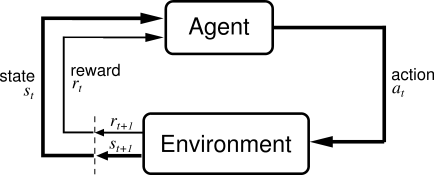
\includegraphics[width=3in]{figures/agent-environment.png}
  \caption{Agent-Environment Interface}
  \label{fig:agent-env}
\end{figure}

% Figure here
In this setting, an agent in a state $s \in \states$ chooses an action
$a \in \actions$, and moves to a state $s'$ with probability
$\transitions(s'|s,a)$, receiving a reward $\rewards(s,a)$
(\autoref{fig:agent-env}). In the fully observable setting, the agent is
aware of which state it is in, and the objective of the agent is to find
a policy $\policy: \states \to \measure( \actions )$, i.e. a decision
procedure for selecting actions, that maximises the reward it
accumulates in the long run, $R = \sum_{i} \gamma^i r_i$. $R$ is also
called the return. 

In the remainder of this section, we will describe the basic approach
for finding an optimal policy $\policy$ for a discrete MDP, and its
continuous variant. 

% Various representations of MDPs

% Discrete MDPs
\subsection{Discrete Markov Decision Processes}
 
In the discrete case, $\states$ and $\actions$ are predictably finite
sets of states and actions. We define the value function $V^{\pi}:
\states \to \Re = \E_{\pi}[\sum_{t=0}^{\infty} \gamma^{t} R_t | S_0
= s ]$ to be the expected return from $s$, and $Q^{\pi}: \states \times
\actions \to \Re = \E_{\pi}[\sum_{t=0}^{\infty} \gamma^{t} R_t | S_0
= s, A_0 = a ]$ to be the expected return from $s$, after taking the
action $a$. These can be written in a recursive form,
\begin{eqnarray*}
  V^{\pi}(s) &=& \max_{a} \rewards(s,a) + \gamma \sum_{s' \in \states} \transitions(s'|s,a) V^{\pi}(s') \\
  Q^{\pi}(s,a) &=& \rewards(s,a) + \gamma \sum_{s' \in \states} \transitions(s'|s,a) Q^{\pi}(s',a').
\end{eqnarray*}

Our objective can then be stated as finding a policy $\pi$ with an
optimal value function, i.e. $V^{*}(s) = \sup_{\pi} V^{\pi}(s)$ at all
$s \in \states$. The optimal value functions must satisfy the Bellman
optimality conditions, 
\begin{eqnarray*}
  V^{*}(s) &=& \max_{a} \rewards(s,a) + \gamma \sum_{s' \in \states} \transitions(s'|s, a) V^{*}(s') \\
  Q^{*}(s,a) &=& \rewards(s,a) + \gamma \sum_{s' \in \states} \transitions(s'|s,a) \max_{a'} Q^{*}(s',a').
\end{eqnarray*}

Given an optimal $Q$, it is possible to construct a greedy policy that
is optimal; $\pi(s,a^*) = 1$ when $a^* = \argmax_{a} Q(s,a)$, and $0$
otherwise. In principle, if the agent knew the MDP, it could construct
the optimal value function, and from it an optimal policy.  However,
in the typical setting, the agent is only aware of the state-action
space, $\states$ and $\actions$, and must learn $Q$ through
exploration. The Q-learning algorithm learns $Q$ with a simple update
for every step the agent takes, $$Q(s,a) = Q(s,a) + \alpha
[ r + \gamma \max_{a'} Q(s',a') - Q(s,a) ],$$ where $\alpha \in [0,1]$
is a parameter that controls the learning rate.  It has been shown
that the Q-learning algorithm converges to the optimal value function
in the limit with fairly permissive assumptions.

% Continuous MDPs
\subsection{Continuous Markov Decision Processes} 

In continuous domains, defining $\states$ and $\actions$ must be done
with some care. To begin with, $\states$ must be a measurable
Euclidean space \footnote{Roughly, a space $X$ is said to be
measurable if a monotonic function $\mu: 2^X \to \Re$ that is additive
over finite union can be defined.}; let us denote the Lebesgue measure
\footnote{The Lebesgue measure is a generalisation of length/area. It
is possible to construct a Lebesgue measure for any Euclidean space.}
by $\lambda$.  Consider the following (mild) regularity assumption
proposed in \citet{Andra2008}, 
\begin{property}(MDP Regularity)
  \label{prop:mdp-regularity}
  $\states$ is a compact subset of the $d_{\states}$-dimensional
  Euclidean space, $\actions$ is a compact subset of $[-A_{\infty},
  A_{\infty}]^{d_{\actions}}$. The random immediate rewards are bounded
  by $\hat{R}_{\max}$ and $\rewards$ is uniformly bounded by $R_{\max}:
  \|r\|_{\infty} \le R_{\max}$.
\end{property}

We define the evaluation operator; $T^{\pi}:B(\states \times \actions)
\to B(\states \times \actions)$, $$ T^{\pi}Q(s,a) = \rewards(s,a)
+ \gamma \int_{\states,\actions} \ud s' \ud a'~ \transitions(\ud
s'|s,a) \pi(a'|s') Q(s',a').  $$ We now define the analogue of the
$Q$-value function recurrence relation, $Q^{\pi} = T^{\pi}Q^{\pi}$.
The fixed point of the Bellman operator $T :B(\states \times \actions)
\to B(\states \times \actions)$, $$ TQ(s,a) = \rewards(s,a) + \gamma
\int_{\states} \ud s'~ \sup_{a' \in \actions} \transitions(\ud s'|s,a)
Q(s',a'),$$ $Q^* = TQ^*$ is then the optimal value function. By the
regularity conditions imposed in \autoref{prop:mdp-regularity},
$V^{\pi}$ and $Q^{\pi}$ are both bounded by $\frac{R_{\max}}{1
- \gamma}$.

In order to approach learning an optimal policy, we must estimate the
current value function, $Q$. One method is to use a function
approximator. Another popular scheme is the Fitted Q-iteration
approach, wherein the $Q$ function is estimated by regressing on
a finite trajectory collected using a stationary policy $\pi_b$. Let
$[S_t, A_t, R_t]_{1 \le t \le N}$, be the dataset, and then $Q_{k+1}$
can be got by, $$Q_{k+1} = \textrm{Regress}( \left\{ [(S_t, A_t), R_t
+ \gamma \max_{a' \in \actions} Q_k(X_{t+1},a')]_{1 \le t \le N-1}
\right\} ).$$

The regression itself can be solved using a variety of methods,
including neural networks and SVMs. A further discussion on suitable
regression methods, and a proof of convergence subject to niceness
assumptions can be found in \citet{Andra2008}.

\section{Spatial Abstractions: Homomorphisms}
\label{sec:background:homs}

% TODO: Clean up.
A homomorphism is defined in general to be a structure-preserving map.
In the context of MDPs, we want a correspondence between the two
systems' dynamics ($\transitions$) and tasks ($\rewards$). 

\begin{definition}(MDP Homomorphism)
An MDP homomorphisms $h$ from an MDP $\mdp = \tuple{S,A,P,R,\gamma}$ to
and MDP $\mdp' = \tuple{S',A',P',R',\gamma}$ is a surjection for the
state-action spaces $S \times A \to S' \times A'$ such that,
\begin{eqnarray}
  P'(h(s,a),\him{s'}) &=& \sum_{s' \in \finv{f}(\him{s'})} P(s,a,s') \label{condition:hom-P} \\
  R'(h(s,a)) &=& R(s,a), \label{condition:hom-R} 
\end{eqnarray}
\noindent
where $f$ is $h$ restricted to $S$, i.e. $f(s) = h(s,a)\mid_S$, and
$\him{s'}$ is the image of $s'$ in $\mdp'$, i.e. $\him{s'} = f(s')$.
\end{definition}

With minor abuse of notation, we assume $P(h(s,a),\him{s'}) \triangleq
P(\him{s}, \him{a}, \him{s'})$, where $h(s,a) = (\him{s}, \him{a})$.
Similarly, $Q(h(s,a)) = Q(\him{s},\him{a})$. For brevity, we will write
$\mdp \hom{h} \mdp'$ if $\mdp'$ is the homomorphic image of $\mdp$ under
$h$. We will also use the notation $(s,a) \in \mdp$ to mean $(s,a) \in
S \times A$. Finally, two state-action pairs $(s,a)$ and $(s',a')$ are
equivalent if $h(s,a) = h(s,a') = (\him{s},\him{a})$. We write this as
$(s,a) \sim (s',a')$.

There can be other, less strict definitions of homomorphisms based on
preserving the value function, policy behaviour, etc. A survey of these
definitions can be found in \cite{Li06}.

% Description of major problems for homomorphisms.
Given this definition, there are perhaps four serious questions that
we wish to answer when talking about homomorphisms,
\begin{enumerate}
  \item (Transfer) Given a homomorphisms $g$ between MDPs $M$ and $M'$,
    can one use a policy learnt in $M$ in $M'$, and vice versa?
  \item (Discovery) Given MDPs $M$ and $M'$, are they homomorphic? 
  \item (Minimisation) Given an MDP $M$, what is the smallest $M'$
    isomorphic to $M$?
  \item (Approximate Minimisation) Given an MDP $M$, and a class of
    homomorphisms $H$, what is the closest approximation $M' \in H(M)$
    of $M$?
\end{enumerate}

All of these questions have been convincingly answered in the case of
discrete MDPs. 

% Description of how homomorphisms can be used to pull back policies 
\subsection{Transferring Policies in Discrete MDPs}

The primary application of MDP homomorphisms is in the transfer of
learning in problem to another. 

\begin{definition}(Lifted Policy)
  Given $\mdp \hom{h} \mdp'$, and a policy $\pi'$ in $\mdp'$ we can
  define a {\em lifted policy} $\pi = \finv{h}(\pi')$ in $\mdp$ as
  follows,
  \begin{eqnarray}
    \pi(s,a) &\triangleq& \frac{\pi'(h(s,a))}{ |\{a':h(s,a') = h(s,a)\}| }. \\
             &=& \frac{\pi'(h(s,a))}{ |\{a':(s,a') \sim (s,a)\}| }.
  \end{eqnarray}

  Note that the denominator equally distributes the selection
  probability between equivalent actions for a state.
\end{definition}

A powerful result that we will later review shows that the lifted
policy of an optimal policy is itself optimal. This is a special case
of the result that the value of the lifted policy is equal through out
$M$ to the value of the original policy in $M'$, i.e. for all $s$,
$V^{\pi}(s) = V^{\pi'}(\him{s})$.

% Description of how homomorphisms can be used in context of relativized options.
\begin{note}(Partial Homomorphisms and Relativised Options)

  \begin{figure}[ht]
    \centering
    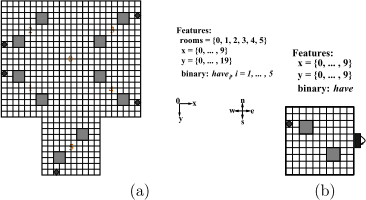
\includegraphics[width=3in]{figures/relativized-options.png}
    \caption{Relativised Options}
    \label{fig:relativised-options}
  \end{figure}

The ability to `lift' policies from one MDP to another can be exploited to
solve subproblems in a reinforcement learning domain. Consider the grid-world
shown in \autoref{fig:relativised-options}(a) taken from \cite{Ravindran2003};
in this domain, there are several rotated copies of the room shown in
\autoref{fig:relativised-options}(b). For each room in (a), let us define a
homomorphism mapping each cell within the room to those of the template room
(b). All states outside the room are mapped to the `sink' state, denoted by the
black square in (b). We can now define {\em options}
\cite{SuttonPrecupSingh1999} for each room, using the optimal policy for (b),
$\pi$, and the above homomorphisms; $\options = \{\finv{h_r}\pi(a) \mid \mbox{for
each room $r$} \}$.

\end{note}

\section{Temporal Abstractions: The Options Framework}
\label{sec:background:options}

The options framework provides a temporal abstraction through subtasks.
An option $\option$ is described by an initiation set $\initset \subset
\states$, a policy $\pi$, and a terminating condition $\beta$.  An agent
can exercise an option in any state $s \in \initset$, following which,
it will follow the policy $\pi$ described by the option, until the
terminating condition $\beta(s)$ is satisfied. The terminating condition
$\beta$ can be stochastic.

Several learning algorithms have been proposed for agents using options
\cite{SuttonPrecupSingh1999,BartoMahadevan2003}. One simple such method that
we will use is MacroQ, a generalisation of the Q-learning algorithm
described above. The MacroQ algorithm updates the value function only
after completion of the option. If the option $o$ was initiated in the
state $s$, and continues for $k$ steps before terminating in $s'$, the
corresponding $Q$ function update will be,
\begin{eqnarray*}
    Q(s,o) &=& Q(s,o) + \alpha [ r + \gamma^{k} \max_{o' \in \actions \cup \options} Q(s',o') - Q(s,o) ].
\end{eqnarray*}

Different tasks in the same domain can be described by different
$\rewards$. Let $\rewards$ be sampled from the family $\Rewards$. Our
objective then is to find a set of options $O$ that reduces the expected
learning time over $\Rewards$.

\begin{example}
  \label{example:taxi}

\begin{figure}[th]
    \centering
    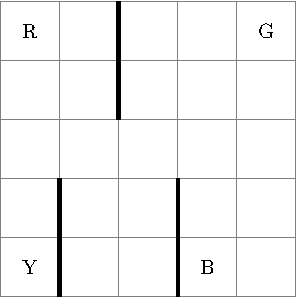
\includegraphics{figures/taxi}
    \caption{The Taxi Domain}
    \label{fig:taxi-domain}
\end{figure}
To make the discussion more tangible, let us look at an example, the
Taxi domain, shown in \figref{fig:taxi-domain}. The agent is a taxi
navigating in this road-map. It must pick up a passenger at one of the
4 pads, R, G, B or Y.  Subsequently, it must carry the passenger to a
destination, which is also one of the above four pads. The states of
the taxi would then be a tuple containing the location of the
passenger (in one of the four pads, or within the taxi), the
destination of the passenger, and location of the taxi in the map.
The actions the taxi can perform are moving up, down, left or right in
the map, as well as pick up or drop a passenger at a pad. 
Typical options for such a domain would be an option that can be
started anywhere, and has a policy that takes the taxi to the one of
the pads in the shortest possible manner. Such an option is generic,
and does not depend on where the passenger or destination are. The RL
agent must then learn to choose the right option when picking up the
passenger.
\end{example}

\section{Small World Networks}
\label{sec:background:sw}

\begin{figure}[ht]
  \centering
  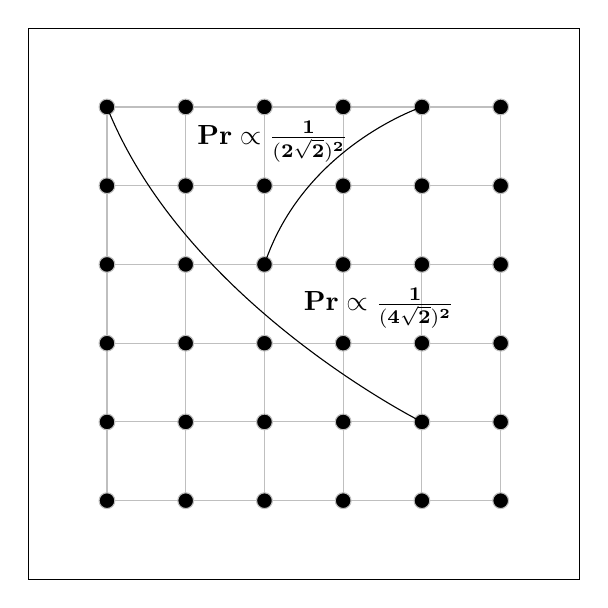
\begin{tikzpicture}[]
    % Grid
    \draw[clip] (-1,-1) rectangle (6,6);
    \draw[step=1,color=lightgray] (0,0) grid (5,5);
    \foreach \xpos in {0, 1, 2, 3, 4, 5}
    {
      \foreach \ypos in {0, 1, 2, 3, 4, 5}
      {
      \draw [color=lightgray,fill=black,opacity=1.0] (\xpos,\ypos) circle (0.1);
      };
    };

    % Draw some long range edges
   \draw (2,3)  .. controls (2.5,4.5) and (4,5) .. node [left] {$\mathbf{Pr \propto \frac{1}{(2\sqrt{2})^2}}$} (4,5);
   \draw (0,5)  .. controls (1.0,2.5) and (4,1) ..  node [above right] {$\mathbf{Pr \propto \frac{1}{(4\sqrt{2})^2}}$} (4,1);

\end{tikzpicture}
  \caption{Kleinberg's Small World Network}
  \label{fig:kleinberg-sw}
\end{figure}

% What are small world options
In Kleinberg's small-world network model (\figref{fig:kleinberg-sw}),
each node $u$ is given one `long-range' edge to a node $v$, which was
chosen with a probability $P_r(u,v) \propto \|u-v\|^{-r}$, where
$\|u-v\|$ denotes the least distance between nodes $u$ and $v$ in the
graph. On an $r$-dimensional lattice, $\klein_r$, the distance from
any node $u$ to a target node $t$ is bounded by $\|u-t\|$, a quantity
which is locally computable. When given long-range edges distributed
according to $P_r$, \citet{Kleinberg2000} showed that a greedy
distributed algorithm $\greedyalgo$ that chooses a neighbour $v$
closest to $t$ will reach $t$ with an expected time $O(\log(|V|)^2)$.
This result is significant because the expected time for the algorithm
on a graph with edges distributed uniformly, i.e. without dependence
on distance, is $O(|V|^2)$.

\begin{theorem}
  \label{thm:kleinberg-sw}
  Let $f: V \to \Re$ be a vertex function, and $M_f$ be the global
  maxima of $f$. Consider an algorithm, \greedyalgo, that greedily
  chooses the neighbour with the highest value of $f$. Suppose the
  algorithm is currently at $u$, it will choose $N(u) = \argmin_v \|f(v)
  - f(M_f)\|$.
  
  If $\graph(V,E)$ is $r$-dimensional lattice, and contains a long
  distance edge distributed according to $P_r: p(u,v) \propto
  \|u-v\|^{-r}$, then \greedyalgo takes $O( (\log |V|)^2 )$ steps to
  reach $M_f$.
\end{theorem}
\begin{proof}
  We defer the proof of this theorem to \secref{sec:sw:theory}, where we
  prove a generalisation of this theorem (\thmref{thm:sw}).
\end{proof}


%\chapter{Related Work}
\label{chap:related-work}

In this chapter we will review existing methods for option-discovery and
transfer learning.

\section{MDP Minimisation and Homomorphism Discovery in Discrete MDPs}
\label{sec:related-work:homs}

In order to answer the minimisation question, Narayanamurthy and
Ravindran reduced the MDP homomorphism query to a graph automorphism
problem in \cite{Narayanamurthy2008} by constructing an equivalent
weighted digraph from an MDP $M \tuple{\states, \actions, \transitions,
\rewards}$. 

We briefly describe the reduction: Construct a graph $G_{M}$, with
$\states$ as nodes. For each node $s$, add an edge to the node $s'$ if
there is some action $a$ that takes the agent from $s$ to $s'$. Each
edge is weighted with the vectors, $\tuple{p_{a_1}, \cdots,
p_{a_|\actions|}}$ and $\tuple{r_{a_1}, \cdots, r_{a_|\actions|} }$,
where $p_{a_i} = \transitions(s, a_i, s')$, and $r_{a_i} = \rewards(s,
a_i, s')$. We could also view this as a construction of two graphs, one
for $\transitions$, and the other for $\rewards$; the graph isomorphisms
we are looking for belong to the common subset.  

There are cases for which using the symmetry group may not suffice to
capture the symmetries present; Section 4.1.1 of \cite{Ravindran2004}
presents one such example. This method can not be extended to continuous
domains easily, as the number of states is no longer countable, and
hence a reduction to a graph isomorphism problem is not possible.

% Description of finding symmetries in discrete case.
\section{Approximate Homomorphisms for Discrete MDPs}

In practice, exact symmetries are rarely found. In such situations,
approximate homomorphisms may be more suitable. The most common approach
is to aggregate states within a certain error bound $\epsilon$ of the
transition and reward functions; this is the approach followed in
\citet{Ravindran2004b} and \citet{Taylor2009}. Both papers also present
a bound on the approximation loss, which is linearly dependent on the
maximum error in expected reward ($R$) and transition probability. 

Another approach to approximate homomorphisms, proposed by
\citet{Sorg2009}, is to probabilistically map states onto the
homomorphic image through ``soft homomorphisms''; i.e. $h: S \to
\measure(S')$, such that,
\begin{eqnarray*}
  \sum_{\him{s} \in S'} P'(\him{s},a,\him{s'}) h(\him{s}|s)  &=& \sum_{s' \in S} P(s,a,s') h(\him{s'}|s') \\
  \sum_{\him{s} \in S'} R'(\him{s},a) h(\him{s}|s)  &=& R(s,a).
\end{eqnarray*}

Finding these soft homomorphisms can be shown to be a quadratic program,
\begin{eqnarray*}
  \forall_a H P'^a &=& P^a H \\
  \forall_a H R'^a &=& R^a \\
  H 1_{|S'|}  &=& 1_{|S|} \\
  H_{ij} &\ge& 0.
\end{eqnarray*}
\noindent
where,
\begin{eqnarray*}
  H: |S| \times |S'| &=& h(\him{s'}|s) \\
  P^a: |S| \times |S| &=& P(s'|s,a) \\
  R^a: |S| \times 1 &=& R(s,a) \\
  P'^a: |S'| \times |S'| &=& P(\him{s'}|\him{s},a) \\
  R'^a: |S'| \times 1 &=& R(\him{s},a).
\end{eqnarray*}

\citet{Sorg2009} further show how soft homomorphisms can be used to map
learning to a scaled up version of the state space, as well as map
a continuous state space to a discrete one. One of the drawbacks of this
approach however, is the lack of state dependent action recoding. 

Of the two approaches, using soft homomorphisms seems more easily
applicable in the continuous domain. In fact, we attempted to approach
the problem in this fashion, however we found the optimisation problem
to be intractable (\secref{sec:alt-hom-approaches:bayesian}).

\section{Option Discovery}
\label{sec:related-work:options}

One of the first option discovery schemes was by \citet{McGovern2001},
who identify states that are visited frequently through an empirical
count. The problem is cast as a multiple-instance learning problem,
where an option or ``concept'' that explains the most number of
successful trajectories is chosen. Our approach of constructing options
from multiple trajectories is similar to \citet{McGovern2001}'s method
of using several trajectories to find the minimal explanation.

\citet{Menache2002} approaches the option discovery also through the
angle of finding bottlenecks. They make the observations that bottleneck
states join well connected regions of the state-space graph, and use
a graph cut algorithm to find bottlenecks, which are nodes in the cut set. 

The state-of-the-art option discovery technique uses the betweenness
scores of states as a measure of importance \citep{Simsek2008}. This is
an intuitive measure, since graph betweenness measures the proportion of
paths that go through a particular node. In a domain like Taxi, the
pickup and drop actions are states with high betweenness values. In
navigational domains likes Rooms, doorways are high betweenness centers.
\citet{Simsek2008} also show how a locally constructed model of the MDP
can be used to compute betweenness scores.

%Shie Mannor
%Betweenness

%\chapter{Searching for Homomorphisms}
\label{chap:hf}

In this chapter, we explore spatial homomorphisms in continuous domains.
We begin by describing the challenges of such a definition
(\secref{sec:hf:continuous-hom}), and describe a extension to existing
MDP homomorphism definitions that tackles them
(\secref{sec:hf:definition}). As an aside, we detail an interesting
family of continuous homomorphisms, namely continuous affine
homomorphisms in \secref{sec:hf:affine}. We develop an online algorithm
to find homomorphisms from this family in
\secref{sec:hf:homomorphic-filters}, and evaluate this algorithm in
\secref{sec:hf:experiments}.

\section{Continuous Homomorphisms}
\label{sec:hf:continuous-hom}

An important property of symmetries in continuous domains is that they
may reduce the dimensionality of the domain; the type of symmetries
present in discrete domains can only ``fold'' the state space in
finitely many ways. To motivate this distinction, consider the following
examples,

\begin{figure}[h]
  \centering
  \subfloat[Discrete Symmetry]{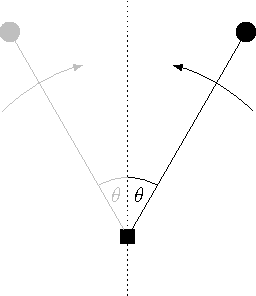
\includegraphics[width=2in]{figures/inverted-pendulum} \label{fig:inverted-pendulum}} \hspace{0.5in} 
  \subfloat[Continuous Symmetry]{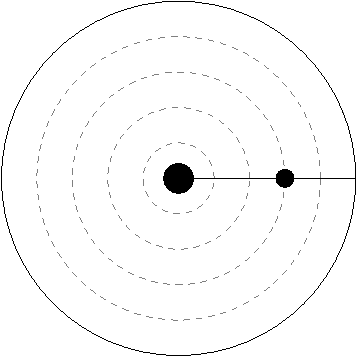
\includegraphics[width=2in]{figures/reach-center} \label{fig:reach-center}} 
%  \subfloat[Octopus Arm: Algebraic (Continuous) Symmetry]{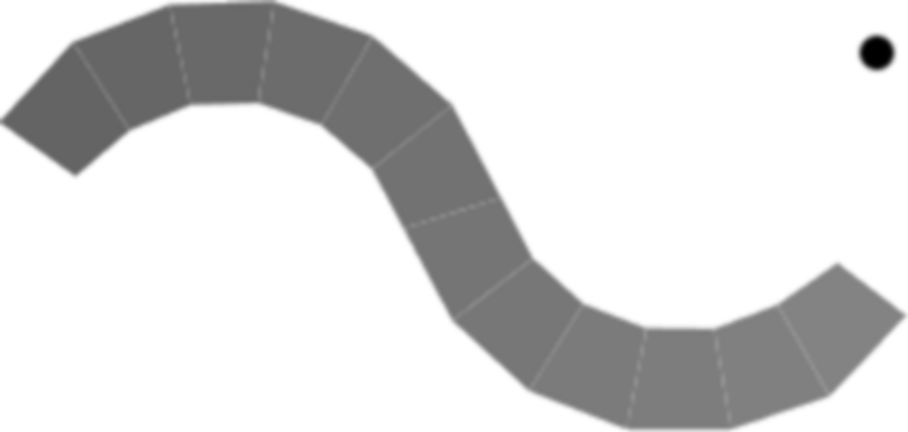
\includegraphics[width=6cm]{figures/octopus} \label{fig:octopus}}
\end{figure}

\subsection{Inverted Pendulum} 
In this example, the agent is aware of a single continuous variable,
the angular displacement of the pole from the vertical, and has either
two discrete actions to move to the left or to the right with
a certain acceleration/impulse, or a continuous range of
acceleration/impulse (\figref{fig:inverted-pendulum}).  There is an
obvious symmetry of reflection about the vertical. This is an example
of a finite symmetry group. The dimensionality of the homomorphic
space remains unchanged.

\subsection{Reach the Center} 
Imagine a circular disc-world wherein an agent must navigate to the
center of the disc. The only relevant variable here is the radial
distance, and all points along a circle with a particular radius are
homomorphically equivalent (\figref{fig:reach-center}). This is an
example of an infinite symmetry group. The dimensionality of the
homomorphic space has reduced to $1$ from $2$. 

In general, the dimensionality of the homomorphic image reduces by the
``height'' of the symmetry group; this is a standard result from
algebra.

\section{Well-Definedness of Continuous MDPs}
\label{sec:hf:definition}

In order to capture continuous symmetries in our framework, we need
a definition of continuous MDP homomorphisms that captures both finite
and infinite pre-images. This problem is resolved if, instead of maps
between points, we considered maps between {\em closed topological
sets}. The circle described in the previous example, while composed of
an infinite number of points is still a closed set, and so is its
image, a single point. Topologically speaking, a map that takes closed
sets to closed sets is continuous. The coincidence that homomorphisms
in continuous domains must themselves be continuous allows us to
unambiguously use the term ``continuous homomorphisms'' in the
sequel.

\begin{definition}(Continuous MDP Homomorphism)
  An continuous MDP homomorphisms $h$ from a continuous MDP $\mdp
  = \tuple{S,A,P,R,\gamma}$ to and a continuous MDP $\mdp'
  = \tuple{S',A',P',R',\gamma}$ is a {\em continuous} surjection $S \times
  A \to S' \times A'$ such that,
  \begin{eqnarray}
    P'(h(s,a),\him{s'}) &=& \int_{\finv{f}(\him{s'})} \ud s' ~ P( s, a, s' ) \label{condition:chom-P} \\
    R'(h(s,a)) &=& R(s,a)  \label{condition:chom-R}, 
  \end{eqnarray}
  \noindent
  where $f$ is $h$ restricted to $S$, i.e. $f(s) = h(s,a)\mid_S$, and
  $\him{s'}$ is the image of $s'$ in $\mdp'$, i.e. $\him{s'} = f(s')$.
\end{definition}

The continuity condition also ensures that $\finv{f}(\him{s'})$ is
a well defined, measurable set. Though $\finv{f}(\him{s'})$ may be
a finite set, we slightly abuse notation and use
$\int_{\finv{f}(\him{s'})}$ uniformly; the integral must be replaced
by a summation in case $\finv{f}(\him{s'})$ is finite.

For the remainder of this section, unless specified otherwise, we will
assume all MDPs and homomorphisms are continuous. The lifted policy of
a continuous MDP is defined as follows.

\begin{definition}(Continuous Lifted Policy)
  Given $\mdp \hom{h} \mdp'$, and a policy $\pi'$ in $\mdp'$ we can
  define a {\em lifted policy} $\pi = \finv{h}(\pi')$ in $\mdp$ as
  follows,
  \begin{eqnarray}
    \pi(s,a) &\triangleq& \frac{\pi'(h(s,a))}{ \int_{\finv{h}_s(\him{a})} \ud a }.
  \end{eqnarray}
  \noindent
  where $\finv{h}_s(\him{a})$ is set of actions equivalent to $a$ in the
  state $s$, i.e. $\{ a \mid h(s,a) = (\him{s},\him{a}) \}$. 
\end{definition}

We will now prove the value equivalence between an continuous MDP and
its homomorphic image and show that the above definitions are sufficient
for this purpose.

\begin{lemma}
  \label{lm:cont-value-eq}
  Let $\mdp \hom{h} \mdp'$. Let $\pi'$ be any policy in $\mdp'$, and
  $\pi$ be its lifted policy in $\mdp'$. Define $V^{\pi}(s) = \int_{A}
  \ud a ~ \pi(s,a) Q^{\pi}(s,a)$. If $Q^{\pi}(s,a) = Q^{\pi'}(h(s,a))$,
  then $V^{\pi}(s) = V^{\pi'}(\him{s})$.
\end{lemma}
\begin{proof}
  This follows directly from the definition of the lifted policy $\pi$. 
  \begin{eqnarray*}
    V^{\pi}(s) &=& \int_{A}\ud a ~ \pi(s,a) Q^{\pi}(s,a) \\
    &=& \int_{A'} \ud \him{a} ~ \int_{\finv{h}_s(\him{a})} \ud a ~ \pi(s,a) Q^{\pi}(s,a) \\
    &=& \int_{A'} \ud \him{a} ~ \int_{\finv{h}_s(\him{a})} \ud a ~ \frac{\pi'(\him{s},\him{a})}{ \int_{\finv{h}_s(\him{a})} \ud a } Q^{\pi'}(\him{s},\him{a}) \\
    &=& \int_{\finv{h}_s (\him{a})} \pi'(\him{s},\him{a}) Q^{\pi'}(\him{s},\him{a}) \\
    &=& V^{\pi'}(\him{s}).
  \end{eqnarray*}
\end{proof}


\begin{theorem}(Continuous Value Equivalence)
  \label{thm:cont-value-eq}
  Let $\mdp \hom{h} \mdp'$. Let $\pi'$ be any policy in $\mdp'$, and
  $\pi$ be its lifted policy in $\mdp'$. For any $(s,a) \in S \times A$,
  $Q^{\pi}(s,a) = Q^{\pi'}(h(s,a))$.
\end{theorem}
\begin{proof}
  Consider the recursive definition of the $m$-step discounted action
  value function, $$Q^{\pi}_m(s,a) = R(s,a) + \gamma \int_{S} \ud s'
  ~ P(s,a,s') \int_{A} \ud a' ~ \pi(s',a') Q^{\pi}_{m-1}(s',a'),$$ with
  $Q^{\pi}_{-1}(s,a) = 0$ for any $(s,a) \in \mdp$. We will also define
  an $m$-step discounted value function $V^{\pi}_m(s) = \int_{A} \ud
  a ~ \pi(s,a) Q^{\pi}_m(s,a).$ We can rewrite the previous equation
  as,$$Q^{\pi}_m(s,a) = R(s,a) + \gamma \int_{S} \ud s' ~ P(s,a,s')
  V^{\pi}_{m-1}(s').$$ 

  For the base case, consider the case when $m = 0$. Then,
  $Q^{\pi}_0(s,a) = R(s,a) = R'(h(s,a)) = Q^{\pi'}_0(h(s,a))$.  Assuming
  $Q^{\pi}_j(s,a) = Q^{\pi'}_j(h(s,a))$ for all $(s,a) \in \mdp$ and all
  $j < m$, we must show that $Q^{\pi}_m(s,a) = Q^{\pi'}_m(h(s,a))$. 
  \begin{eqnarray*}
    Q^{\pi}_m(s,a) &=& R(s,a) + \gamma \int_{S} \ud s' ~ P(s,a,s') V^{\pi}_{m-1}(s') \\
    &=& R(s,a) + \gamma \int_{S'} \ud \him{s'} ~ ( \int_{\finv{f}(\him{s'})} \ud s' ~ P(s,a,s') ) V^{\pi'}_{m-1}(\him{s'}) \\
    &=& R'(h(s,a)) + \gamma \int_{S'} \ud \him{s'} ~ P'(h(s,a),\him{s'}) V^{\pi'}_{m-1}(\him{s'}) \\
    &=& Q^{\pi'}_m(h(s,a)).
  \end{eqnarray*}

  Given that $Q^*(s,a) = \lim_{m \to \infty} Q_m(s,a)$, we have
  $Q^*(s,a) = Q^*(h(s,a))$.
\end{proof}

\subsection{Continuous Affine Homomorphisms}
\label{sec:hf:affine}

An interesting family of homomorphisms that we will consider in detail
are that of continuous {\em affine} homomorphisms. These homomorphisms
relate two spaces through a combination of rotation and translation.
A continuous affine homomorphism is parameterised by $A$, an
orthogonal matrix corresponding to rotation, and $b$ a vector
corresponding to translation. In addition, we can project the rotated
vector to a smaller state space with the rectangular identity matrix,
$I_{m,n}$, where $m$ and $n$ are the dimensions of $\mdp'$ (the image)
and $\mdp$ respectively. Thus, $h(x) = I_{m,n} A x + b$.

\begin{example}(Expressive Power of Continuous Affine Homomorphisms)
\begin{figure}[h]
  \centering
  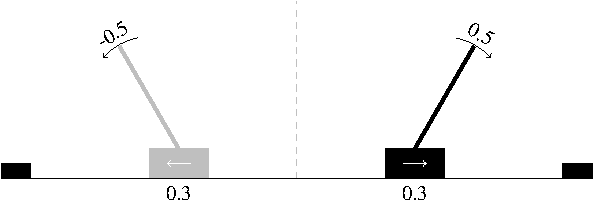
\includegraphics[width=4in]{figures/cart-pole}
  \caption{Cart Pole}
  \label{fig:cart-pole} 
\end{figure}

Let us study the capabilities of the continuous affine homomorphism
family, with the Cart Pole task as an example (\figref{fig:cart-pole}).
In this task, the agent must balance a pole on a cart without moving the
cart out of the boundaries; the only action the agent can perform is to
push the cart forward or backward with some force. The state variables
are the $x$ position of the agent, the angular displacement from the
vertical, and the linear and angular velocities of the cart and pole
respectively.

In a bounded domain, there is a single exact automorphism; a reflection
of all the state features about the centre of the track. This instance
is trivially captured by the continuous affine family, $A = -I$ and $b
= 0$. In an unbounded domain, however, the whole system is
translation-invariant, i.e. the $x$ position does not matter. In such
a case, $A$ could zero out the contribution of $x$, and $b$ translate
the system to any coordinate. This homomorphism is a reasonable
approximation even in bounded domains.

An interesting reduction we could study in this domain would be to
project the angular state space coordinates, and lift a policy from an
inverted pendulum. $A$ is simply the permutation matrix that shifts the
angular components to the first two features.
\end{example}

\section{Homomorphic Filters}
\label{sec:hf:homomorphic-filters}

% Exact symmetry -> Approximate symmetry
A number of factors make searching for exact homomorphisms impractical.
Rarely is the environment model exactly known, particularly in some
closed form that it can be exploited. Furthermore, exact homomorphisms
are extremely sensitive to noise, thus rendering them inapplicable to
any learnt models. Given these conditions, it is more prudent to search
for approximate homomorphisms. In this section, we describe an online
algorithm to find homomorphisms from the current environment, $\mdp$, to
an environment the agent has encountered before, $\mdp'$. We assume that
we have a model of $\mdp'$, but not of $\mdp$. 

% While experience from $\mdp'$ can be used to learn $\mdp$ more
% effectively, we can not rely on any model of $\mdp$ until there have
% been enough steps to obviate the need for it!

In principle, we would like to find a homomorphism that minimises the
expected difference between $x' \sim P_{\mdp}(x,a)$ and $\him{x'} \sim
P_{\mdp'}(h(x,a))$, as well as $R_{\mdp}(x,a)$ and $R_{\mdp'}(h(x,a))$.
To this end, we propose the following objective function,
\begin{eqnarray}
  C(h) &=& \int_{\states \times \actions} \ud x \ud a ~ C(h,x,a) \label{eq:hf:cost}\\
  C(h,x,a) &=& \half \E[ (\him{x'} - h(x'))^2 ] + \half \E[ (R_{\mdp'}(\him{x}) - R_{\mdp}(x))^2 ] \nonumber.
\end{eqnarray}

Without a model for $\mdp$, the above expectations can not be evaluated,
let alone minimised. However, we can use samples of $x$, $a$, $x'$ and
$r$ collected by the agent's interaction with the world to perform
stochastic gradient descent,
\begin{eqnarray*}
  h_{t+1} &\gets& h_{t} - \alpha \innerprod{\grad_h C(h,x,a)}{\homset} \\
  \grad_h C &=& \half \grad_h [ \Tr( K( h(x) ) ) + ( m( h(x) ) - h(x') )^2 + ( R(h(x')) - r )^2   ] \\ 
  \grad_h C &=& \half \grad \Tr( K(h(x)) )\cdot \grad_h h(x) + (m(h(x)) - h(x')) ( \grad m(h(x)) \cdot \grad_h h(x) - \grad_h h(x') )  \\
            &+& ( R(h(x')) - r ) \grad R( h(x') )\cdot \grad_h h(x').
\end{eqnarray*}
$m$ and $K$ are the mean and co-variance of $\mdp'$. Note that we
project the updates onto $\homset$, $\innerprod{\grad_h
C(h,x,a)}{\homset}$.

Finally, as $C(h)$ is in general a complex non-convex function, we
perform the stochastic gradient descent simultaneously on a number of
starting points, or particles. The algorithm is summarised in
\algoref{algo:homo-pf}. The $Q$-value at any point of the homomorphic
filter is computed as an expectation over each particle, with
probabilities proportional to $\exp(-\frac{C(\tilde{h}^j,x,a)}{\tau})$.

\begin{algorithm}[ht]
  \DontPrintSemicolon
  Initialise $M$ particles $h_0^{(i)}$ randomly from $\homset$ \;
  \While{ not converged }{
  \lForEach{particle $i$}{$\tilde{h}_{t+1}^i \gets h_{t}^i + \alpha \innerprod{\grad_h C}{\homset}$} \;
  \lForEach{particle $i$}{$h_{t+1}^i \sim \tilde{h}_{t+1}$ with probability $\propto \exp(-\frac{C(\tilde{h}^j,x,a)}{\tau})$}
  }
  \caption{Homomorphic Filtering}
  \label{algo:homo-pf}
\end{algorithm}

\subsection{Continuous Affine Homomorphisms}
One possible choice for $\homset$ is the set of affine transformations
between the state spaces, i.e. $h(x) = I_{m,n} A x + b$, where $m$ and
$n$ are dimensions of $\mdp'$ and $\mdp$ respectively, $A$ is an
arbitrary orthogonal matrix, and $b$ is an arbitrary translation. Below,
we derive the necessary update equations for this family of
homomorphisms,
\begin{align*}
  \diff{A_{ij}} h(x) &= I_{m,n} 1_i x_j  & \diff{A} f(h(x)) &= \grad f(h(x)) I_{m,n} x^T  \\
  \diff{b_i} h(x) &= 1_i & \diff{b} f(h(x)) &= \grad f(h(x)).
\end{align*}

\begin{eqnarray*}
  \diff{A} C &=& \half \grad \Tr( K(h(x)) ) x^T + \sum_i (m_i(h(x)) - h(x')) (\grad m_i(h(x)) \cdot I_{m,n}^T x^T - 1 \cdot I_{m,n}^T x'^T) \\
             &+& (R(h(x')) - r) \grad R( h(x') ) I_{m,n} x'^T \\
  \diff{b} C &=& \sum_i ( \half \grad K_i(h(x)) + ( m_i(h(x)) - h(x')) (\grad m_i(h(x)) - 1) ) \\
             &+& (R(h(x')) - r) \grad R( h(x') ).
\end{eqnarray*}

The new $A$ can be projected onto the set of orthogonal matrices, by
finding the nearest orthogonal matrix, $A (A^T A)^{-\half}$.

\section{Experimental Results}
\label{sec:hf:experiments}
% Experimental results

%Random orthogonal matrices were generated using Stewart's algorithm (1980).

We evaluated our algorithm on the Cart Pole domain. The domain
describes an agent that must balance a pole on a cart by applying
a linear force to the cart. The domain has four state variables,
$\theta$, the angular displacement of the pole from the vertical, $x$
the linear displacement of the cart from the center, and their
derivatives, $\dot{\theta}$ and $\dot{x}$. The linear force the agent
can apply is discretised into 4 actions. 

We used fitted Q-iteration with support vector regression through out
the experiments to learn the value function. We initially chose Gaussian
process regression to learn the domain models because it provided
a covariance function. However, despite the uniform noise in our
experiments, and hence independence from coordinates, the learnt models
did not accurately predict the variance, and led to greater variability
in performance.  We decided to omit the contribution of variance to the
gradient descent updates, and used the models learnt using support
vector regression for the remainder of the experiments for efficiency
reasons.

The Cart Pole domain has a single exact homomorphism which is a complete
reflection of the coordinates, and reversal of the forces applied. Since
the action space is discrete, we also added {\em an action permutation}
to each particle. Our algorithm found homomorphisms which a combination
of reflections of the angular components, and linear displacements of
cart along the track, both of which are intuitive. When the track on
which the cart moves is bounded, any two positions along the track,
except for mirror reflections, are {\em not} equivalent. However, the
difference in their values is reduces as the cart moves away from the
wall; in limiting case, when the track is unbounded, the $x$
displacement indeed does not matter. 

\begin{table}[hbtp]
%  \floatconts
  \centering
  \begin{tabular}{llll}
  \toprule
  \bfseries $l$, $m_p$, $m_c$ & \bfseries Using Original $\pi$ & \bfseries Using HF $\pi$ & \bfseries New Agent  \\
  \midrule
   $0.5$, $0.1$, $1.0$ & -11.003 & 1.612 & 2.079 \\
  \bottomrule
  \end{tabular}
  \caption{Lifted Policy on Perturbed Domain (Return after $1,600$ epochs)}
  \label{tbl:perturbed-values}
\end{table}

We perturbed the domain by changing some of its parameters (e.g. length
of the pole, masses, etc.), as well as by rotating the state space
coordinates, and observed the performance of the algorithm. We present
the return accumulated by the agent after $1,600$ epochs observations in
\autoref{tbl:perturbed-values}; in general, the lifted policy of the
homomorphic filter was competitive to a trained agent on the perturbed
domain, considerably better than the trained agent in the original
domain.

\begin{figure}
  \centering
  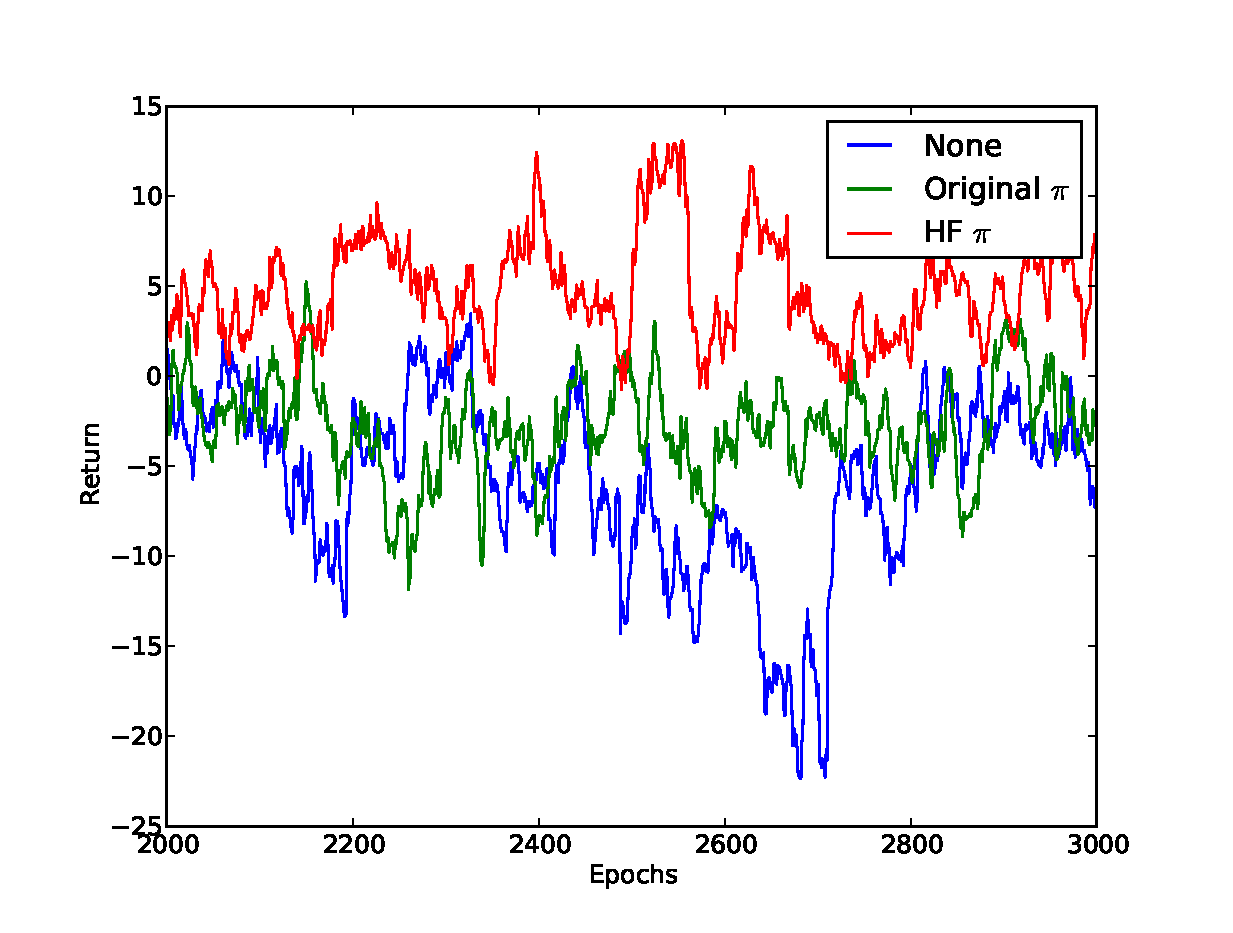
\includegraphics[width=4in]{figures/bootstrap}
  \caption{Bootstrapping Learning in a Perturbed Domain}
  \label{fig:bootstrap}
\end{figure}

We also evaluated the benefit of using the homomorphic filter to
bootstrap the agent using a slight variant of multiple model
reinforcement learning \citep{Doya2002}. Initially, the agent relies
more on the policy of the homomorphic filter, but as the agent's value
function estimate improves, it gradually begins to use its value
function more (\figref{fig:bootstrap}). We compared the performance of
an agent learning without any other model (None), with the policy learnt
in the original task (Original $\pi$), and the policy recommended by the
homomorphic filter (HF $\pi$). The agent using the homomorphic filter
significantly outperforms the other two agents. Note that the agent
using the original policy without any homomorphisms actually negatively
effects the learning of the agent.

%We also learnt a separate model of an inverted pendulum (without
%a cart), and provided the agent with this model.


%\chapter{Small World Options}
\label{chap:sw}

In this chapter, we describe how an MDP can be viewed as a graph, and
how Kleinberg's small-world model can be adapted to this setting
(\secref{sec:sw:graph-view}). We then prove that small world options
indeed guarantee a logarithmic bound on the number of decisions taken by
the agent (\secref{sec:sw:theory}). In line with our general theme of
abstraction learning schemes relying only information readily available
to the agent, we describe an efficient algorithm to learn small world
options completely through trajectories taken by the agent
(\secref{sec:sw:algo}). Finally, we evaluate the small world options,
comparing the options against another state of the art technique in
\secref{sec:sw:experiments}.

\section{Graph View of MDPs}
\label{sec:sw:graph-view}

\begin{figure}[th]
    \centering
    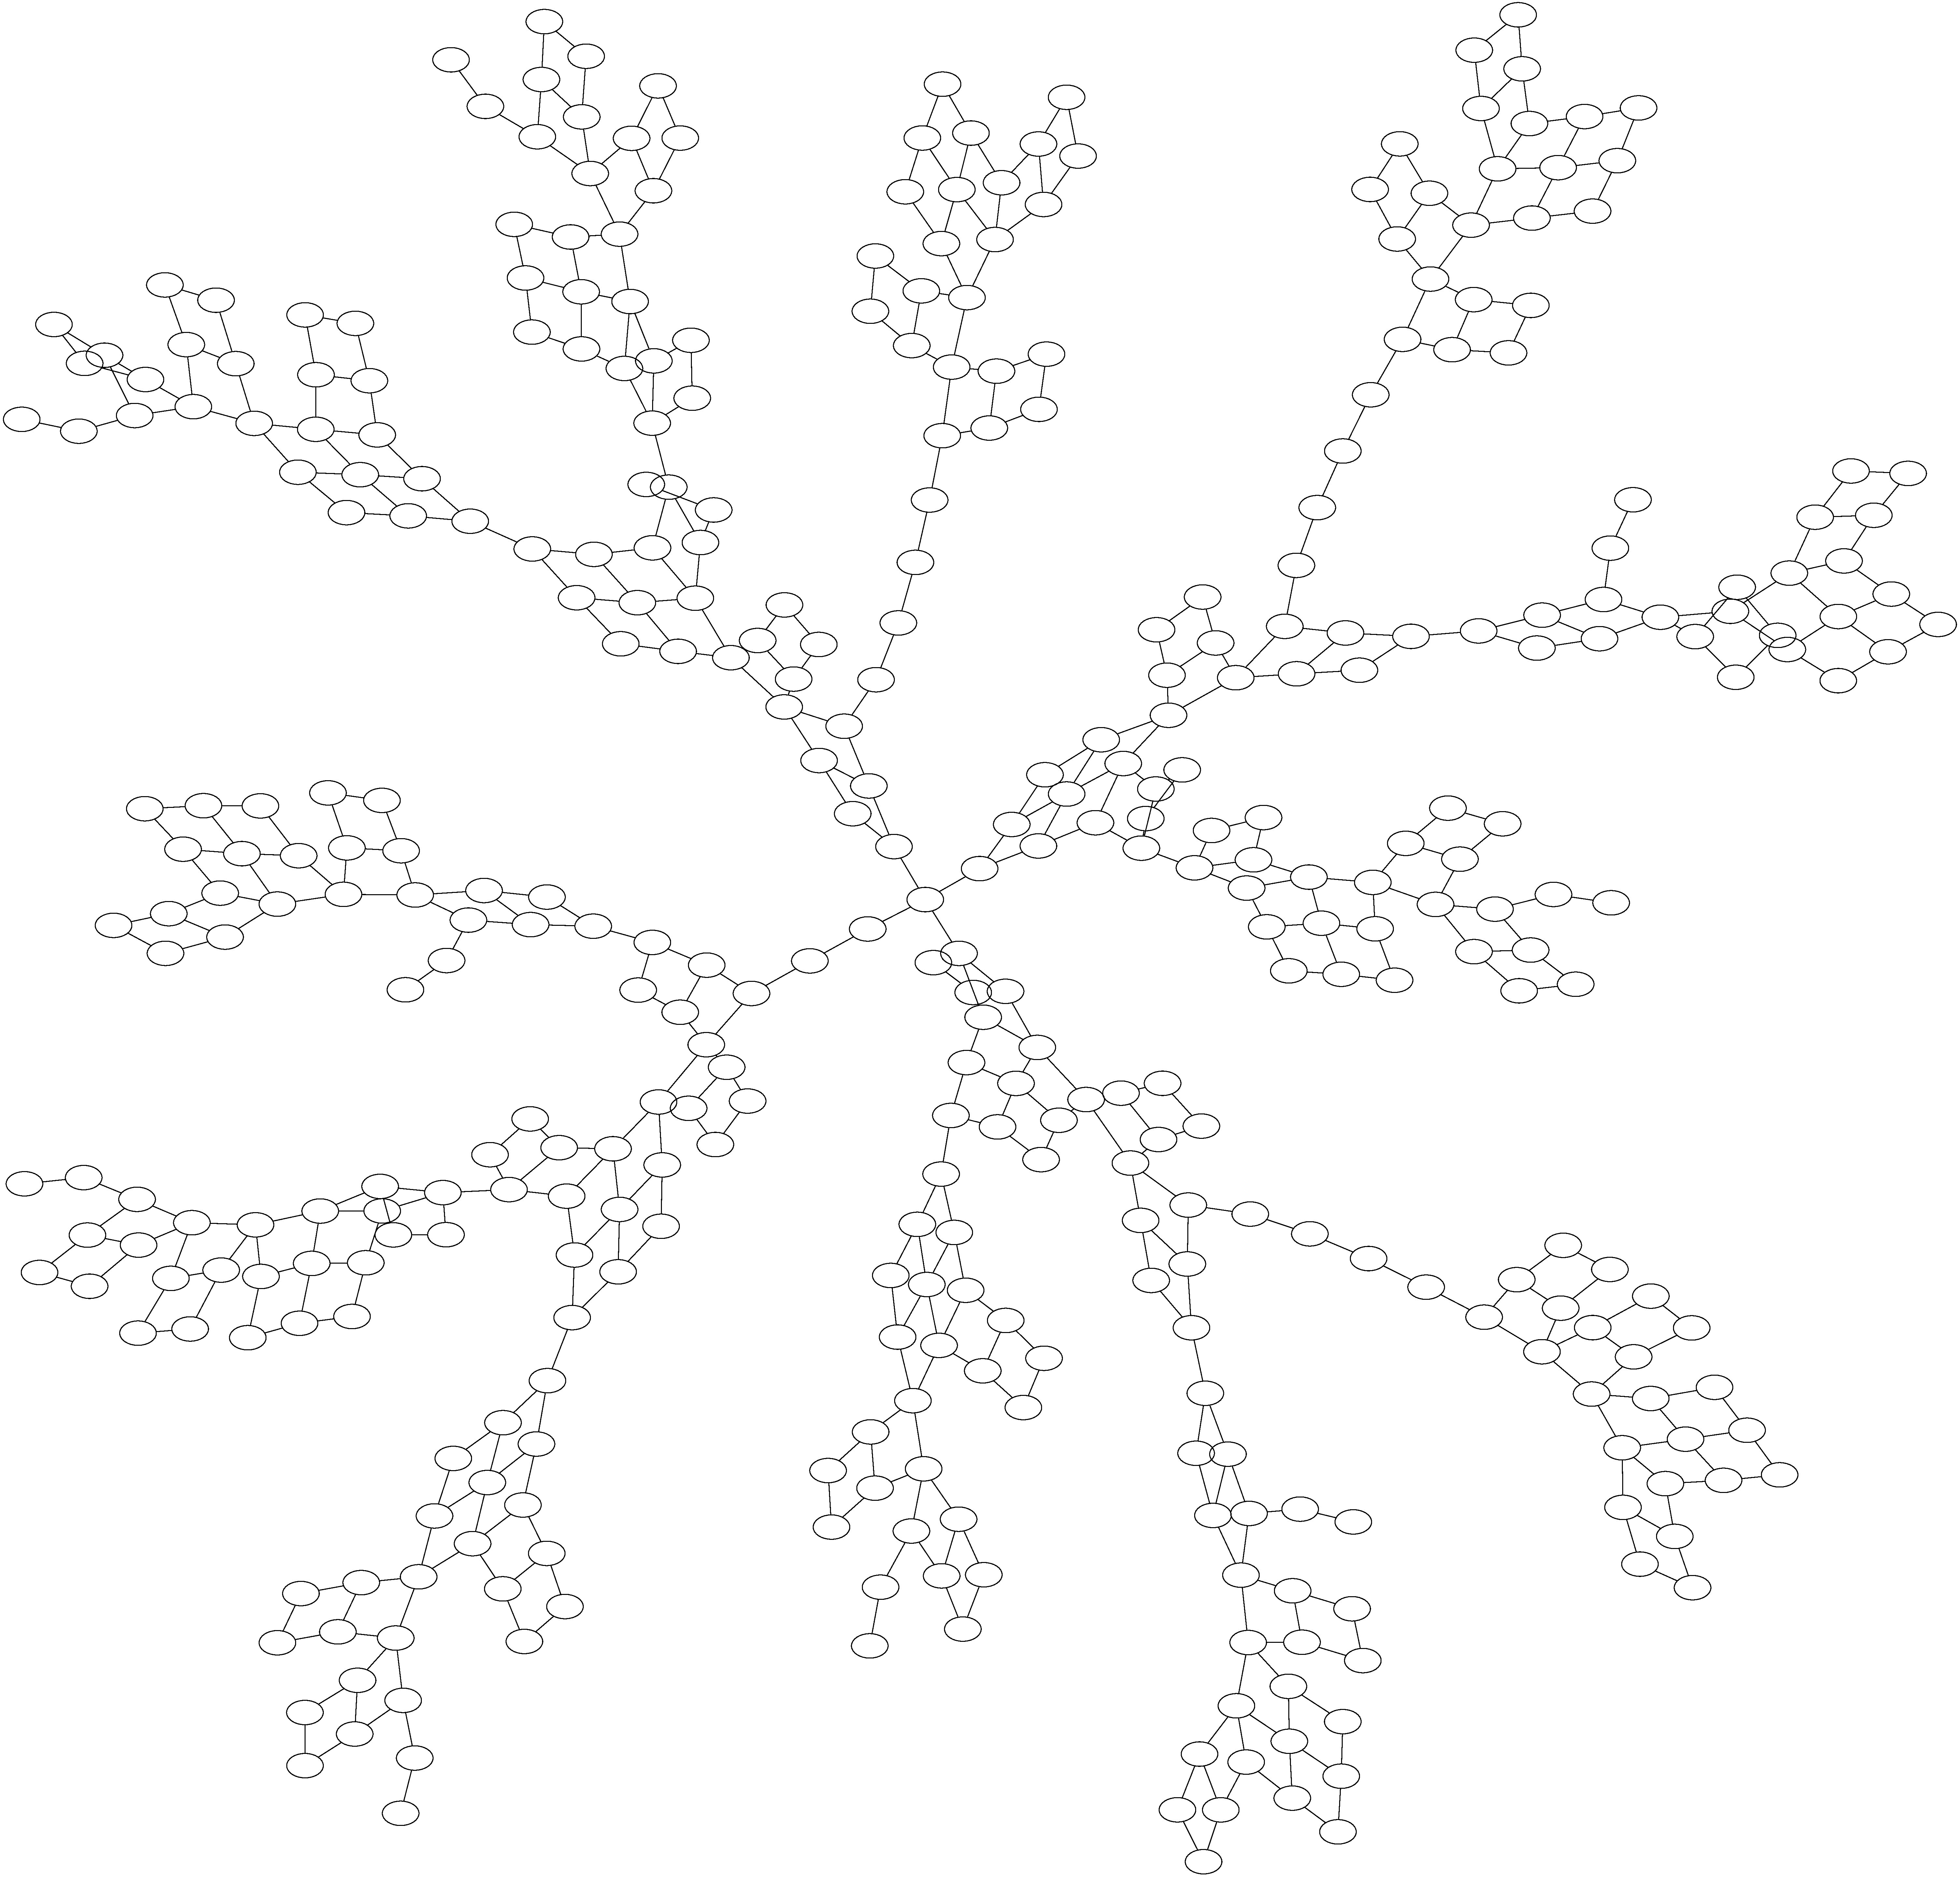
\includegraphics[height=3in]{figures/taxi1}
    \caption{The State Space Graph for Taxi}
    \label{fig:taxi-graph}
\end{figure}

% Graph-based
It is easy to construct a graph $\graph_{\mdp}$ out of the state-space
described by an MDP. The states $\states$ become the nodes of the graph,
and actions $\actions$ become the edges, with the transition
probabilities as weights. Options can be viewed as paths along the
graph. The Taxi domain defined earlier
(\hyperref[example:taxi]{Example~\ref*{example:taxi}}) translates to the
graph shown in \figref{fig:taxi-graph}.

We draw a parallel to the network structure in Kleinberg's small-world
network model (\figref{fig:kleinberg-sw}), by adding a single `path
option' from each state $s$ to another state $s'$, where $s'$ is chosen
with probability $P_r(s,s') \propto \|s-s'\|^{-r}$.  A path option
$o_p(s,s')$ is an option with $\initset = \{s\}$, $\stopcond = \{s'\}$,
and an optimal policy to reach $s'$ for $\pi$.  Intuitively, it is an
option that takes the agent from $s$ to $s'$. In practice, we may
generate path options for only a subset of $|S|$. Note that while this
results in $O(|S|)$ options, only one additional option is available in
any state, and thus the decision-space for the agent is not
significantly larger.

\section{Small World Structure in MDPs}
\label{sec:sw:theory}

Consider an MDP $\mdp_{\klein_r}$ with states connected in
a $r$-dimensional lattice, and noisy navigational actions between
states. We claim that by using {\em robust} path options distributed
according to $P_r$, an $\epsilon$-greedy agent can reach a state of
maximal value using $O(\log(|S|)^2)$ options, using the value function
$\Vf$ as a local property of the state. 

\begin{definition}
    A {\em robust path option} $o(u,v)$, where $u,v \in \states$ is an
    option that takes the agent from $u$ to $v$ `robustly', in the
    sense that in each epoch, the agent moves closer to $v$ with a
    probability $1-\epsilon > \frac{1}{2}$. \footnote{This condition
    is equivalent to saying that the option takes the agent from $u$
    to $v$ in finite time, and hence is not particularly strong.}.
    Note that this $\epsilon$ includes any environmental effects as
    well.
\end{definition}

In order to handle the $\epsilon$-greedy nature of the algorithm, as
well as the approximate-ness in the distance, we will need to extend
Kleinberg's theorem (\thmref{thm:kleinberg-sw}).

\begin{theorem}
  \label{thm:sw}
  Let $f : V \to \Re$ be a function embedded on the graph $\graph(V,E)$,
  such that, $\kappa_1 \|u-v\| - c_1 \le \|f(u) - f(v)\| \le \kappa_2
  \|u - v\| - c_2$, where $0 \le \kappa_1 \le \kappa_2$, and $0 \le c_2
  \le \frac{c_1}{2}$. Let $M_f$ be the global maxima of $f$. Let
  \egreedyalgo be an $\epsilon$-greedy algorithm with respect to $f$,
  i.e.  an algorithm which chooses with probability $1-\epsilon$ to
  transit to the neighbouring state closest to $M_f$, i.e. $N(u)
  = \argmin_v \|f(v) - f(M_f)\|$.
  
  If $\graph(V,E)$ is $r$-dimensional lattice, and contains a long
  distance edge distributed according to $P_r: p(u,v) \propto
  \|u-v\|^{-r}$, then \egreedyalgo takes $O( (\log |V|)^2 )$ steps to
  reach $M_f$.
\end{theorem}
\begin{proof}

This result is a simple extension of Kleinberg's result in
\cite{Kleinberg2000}, and follows the proof presented there, albeit with
the somewhat cleaner notation and formalism of \cite{Martel2004}. We
begin by defining the necessary formalism to present the proof.

\begin{definition}
Let us define $\ball_l(u)$ to be the set of nodes contained within
a ``ball'' of radius $l$ centered at $u$, i.e.  $\ball_l(u) = \{ v \mid
\|u - v\| < l \}$, and $\sball_l(u)$ to be the set of nodes on its
surface, i.e. $\sball_l(u) = \{ v \mid \|u - v\| = l \}$.

Given a function $f:V \to \Re$ embedded on $\graph(V,E)$, we analogously
define $\ballf_l(u) = \{ v \mid |f(u) - f(v)| < l \}$. For notational
convenience, we take $\ballf_l$ to be $\ballf_l(M_f)$.
\end{definition}

The inverse normalised coefficient for $p(u,v)$ is, 
\begin{eqnarray*}
    c_u &=& \sum_{v \ne u} \|u - v\|^{-r} \\
        &=& \sum_{j=1}^{r(n-1)} \sball_j(u) j^{-r}.
\end{eqnarray*}

It can easily be shown that the $\sball_l(u) = \Theta( l^{k-1} )$.
Thus, $c_u$ reduces to a harmonic sum, and is hence equal to $\Theta(
\log n )$. Thus, $p(u,v) = \|u - v\|^{-r} \Theta(\log n)^{-1}$.

\begin{figure}[tbh]
  \centering
    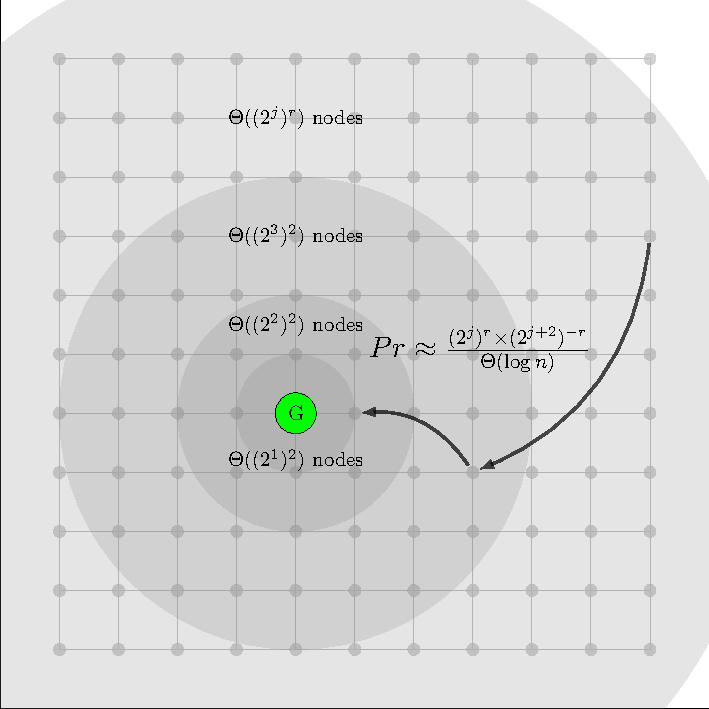
\includegraphics[width=4in]{figures/graph-proof}
    \caption{Exponential Neighbourhoods}
    \label{fig:graph-proof}
\end{figure}

We are now ready to prove that \egreedyalgo takes $O( (\log |V|)^2 )$
decisions. The essence of the proof is summarised in
\figref{fig:graph-proof}. Let a node $u$ be in phase $j$ when $u \in
\ballf_{2^{j+1}} \setminus \ballf_{2^{j}}$. The probability that phase
$j$ will end this step is equal to the probability that $N(u) \in
\ballf_{2^{j}}$. 

The size of $\ballf_{2^{j}}$ is at least $|\ball_{\frac{
2^{j}+c_2}{\kappa_2}}| = \Theta(\frac{2^{j}+c_2}{\kappa_2})$. The
distance between $u$ and a node in $\ballf_{2^{j}}$ is at most
$\frac{2^{j+1} + c_1}{ \kappa_1 } + \frac{2^{j} + c_2}{\kappa_2}
< 2(\frac{2^{j+1} + c_2}{\kappa_2})$. The probability of a link between
these two nodes is at least $(\frac{2^{j+2} + 2 c_1}{\kappa_1})^{-r}
\Theta(\log n)^{-1} $. Thus, 

\begin{eqnarray*}
    P(u, \ballf_{2^{j}} ) &\ge& \frac{(1-\epsilon)}{\Theta( \log n )} (\frac{2^{j}+c_2}{\kappa_2})^{r} \times (\frac{2^{j+2} + 2 c_1}{\kappa_1})^{-r} \\
    &\ge& \frac{(1-\epsilon)}{\Theta( \log n )} \times (\frac{\kappa_1}{4\kappa_2} )^{r} \times ( \frac{ 1 + \frac{c_2}{2^{j}} }{ 1 + \frac{c_1}{2 \times 2^{j}} })^{r}\\
    &\ge& \frac{(1-\epsilon)}{\Theta( \log n )} \times (\frac{\kappa_1}{4\kappa_2} )^{r} \times ( \frac{ 1 + c_2 }{ 1 + \frac{c_1}{2} })^{r} .\\
\end{eqnarray*}

Let number of decisions required to leave phase $j$ be $X_j$. Then, 
\begin{eqnarray*}
    \E[X_j] &\le& \sum_{i=0}^{\infty} (1 - P(u, \ballf_{2^{j}} ))^i \\
            &\le& \frac{1}{P(u, \ballf_{2^{j}} )} \\
            &\le& \Theta( \log n ) \frac{1}{(1-\epsilon)} (\frac{4 \kappa_2}{\kappa_1})^{r} ( \frac{ 1 + \frac{c_1}{2} }{ 1 + c_2 })^{r}\\
            &\le& \Theta( \log n ).
\end{eqnarray*}
Thus, it takes at most $O(\log n)$ decisions to leave phase $j$. By construction, there are at most $\log n$
phases, and thus at most $O((\log n)^2)$ decisions.
\end{proof}

All that remains is to bound the value function, $\Vf$, in terms of the
graph distance to the value maxima. We show this in the following lemma.

\begin{lemma}
    \label{lm:distance}
    Let $o(u,v)$ be the preferred option in state $u$, and let $\|u -
    v\|_V = |\log \Vf(v) - \log \Vf(u)|$. Then, 
    \begin{align*}
        k_1 \|u - v\| - c_1 & \le & \|u - v\|_V & \le & k_2 \|u - v\|, 
    \end{align*}
    \noindent
    where $k_1 = \log \frac{1}{\gamma} $, $k_2 = \log
    \frac{1}{(1-\epsilon)\gamma}$, and $c_1 = \log
    \frac{1}{1-\gamma}$.
\end{lemma}
\begin{proof}
    From the Bellman optimality condition, we get the value of $o(u,v)$ to be,
    \begin{eqnarray*}
        \Qf(u, o(u,v)) &=& \E_{l}[ \gamma^{l} \Vf(v) + \sum_{i=1}^{l} \gamma^{i-1} r_i ],
    \end{eqnarray*}
    \noindent
    where $l$ is the length of the option, and $r_i$ is the reward
    obtained in the $i$-th step of following the option. 
    
    If o(u,v) is the preferred option in state $u$, then $\Vf(u) =
    \Qf(u, o(u,v))$.  Using the property that $0 \le r_i \le 1$,
    \begin{align}
        \E_{l}[ \gamma^{l} \Vf(v) ] &\le& \Vf(u) &\le& \E_{l}[ \gamma^{l} \Vf(v) + \sum_{i=1}^{l} \gamma^{i-1}] \nonumber \\
        \E_{l}[ \gamma^{l} ] \Vf(v) &\le& \Vf(u) &\le& \E_{l}[ \gamma^{l} ] \Vf(v) + \frac{1}{1 - \gamma}. \label{eq:v-bound}
    \end{align}

    $\E_{l}$ is an expectation over the length of the option. Using
    the property that $o(u,v)$ is robust, we move closer to $v$ with
    probability $\epsilonm = 1 - \epsilon$; this is exactly the setting of the
    well-studied gambler's ruin problem, where the gambler begins with
    a budget of $\|u-v\|$, and wins with a probability of $\epsilon$.
    Using a standard result from Feller\cite{Feller1968}, with $m
    = \|u-v\|$, we have,
    \begin{eqnarray*}
        E_l[x^l] = \sum_{l=0}^{\infty} P(L = l) x^{l} &=& \frac{1}{\lambda_1^m( x ) + \lambda_2^m( x )},
    \end{eqnarray*}
    \noindent
    where $\lambda_1(x) = \frac{1 + \sqrt{1 - 4\epsilon\epsilonm
    x^2}}{2\epsilonm x}$, and $\lambda_2(x) = \frac{1 - \sqrt{1
    - 4\epsilonm\epsilon x^2}}{2\epsilonm x}$. When $x \le 1$, 
    \begin{align*}
        \frac{1}{ (\lambda_1( x ) + \lambda_2( x ) )^{m} }  &\le&  E_l[x^l] &\le& \sum_{l=m}^{\infty} P(L = l) x^{l} \\
        \frac{1}{(\frac{2}{2\epsilonm x})^m}  &\le&  E_l[x^l] &\le& \sum_{l=m}^{\infty} P(L = l) x^{m} \\
        (\epsilonm x)^m  &\le&  E_l[x^l] &\le& x^m.
    \end{align*}

    Substituting $x = \gamma$ and $m = \|u - v\|$ into
    \eqnref{eq:v-bound}, we get,
    \begin{align*}
        \E_{l}[ \gamma^{l} ] \Vf(v) &\le& \Vf(u) &\le& \E_{l}[ \gamma^{l} ] \Vf(v) + \frac{1}{1 - \gamma} \\
        (\epsilonm \gamma)^{\|u-v\|} \Vf(v) &\le& \Vf(u) &\le& \gamma^{\|u-v\|} \Vf(v) + \frac{1}{1 - \gamma} \\
        \|u-v\| \log \frac{1}{\gamma} - \log \frac{1}{1-\gamma} &\le& \|u - v\|_V &\le& \|u-v\| \log \frac{1}{\epsilonm \gamma}.
    \end{align*}
\end{proof}

Thus, an $\epsilon$-greedy agent acting with respect to its value
function can reach the maxima of the value function using just $O((\log
|S|)^2)$ decisions. Though this result strictly applies only to the
lattice setting, we observe that many MDPs are composed of lattice-like
regions of local connectivity connected via bottleneck states. The
presence of such bottleneck states would only increase the expected time
by a constant factor. 

\section{Efficiently Constructing Small World Options}
\label{sec:sw:algo}

In \secref{sec:sw:theory}, we remarked that we needed $O(|S|)$ options.
In order to be practical, we require an algorithm to efficiently
generate these options within a budget of training epochs. The proof of
\thmref{thm:sw} provides us with a crucial insight -- our options only
need bring the agent into an exponentially smaller {\em neighbourhood}
of the maximal value state. This suggests that cheaply generated options
may still be acceptable.

The algorithm (\algoref{algo:small-world-experience}) we propose takes
a given MDP $\mdp$, and trains an agent to learn $T$ different tasks
(i.e. different $\rewards$) on it, evenly dividing the epoch budget
amongst them. With each learned task, we certainly will have a good
policy for path options from any state to the state of maximal value,
$M_v$.  However, we observe that will also have a good policy for path
options from $u$ to $v$ is the path is `along the gradient' of $Q$, i.e.
when $V(u) < V(v) < V(M_v)$. Observing that $V(s) \approx \argmax_{v}
Q(s,\pi(s))$, we detail the algorithm to construct many options options
from a single $Q$-value function in \algoref{algo:qoptions}. 

\begin{algorithm}[ht]
  \SetKwInOut{Input}{input}\SetKwInOut{Output}{output}
  \DontPrintSemicolon
  \Input{ $\mdp$, $\Rewards$, $r$, $n$, epochs, $T$ }

  $O \gets \emptyset$ \;
  \For{ $i\gets0$ \KwTo $T$ }{
    $\rewards \sim \Rewards$ \;
    $Q \gets $ Solve $\mdp$ with $\rewards$ using $\frac{\textrm{epochs}}{T}$ epochs \;
    $O' \gets $ QOptions( $Q$, $r$, $\frac{n}{T}$ ) \;
    $O \gets O \cup O'$ \;
  }
  \Return{ A random subset of $n$ options from $O$ }
  \caption{Small World Options from Experience}
  \label{algo:small-world-experience}
\end{algorithm}

\begin{algorithm}[H]
  \SetKwInOut{Input}{input}\SetKwInOut{Output}{output}
  \DontPrintSemicolon
  \Input{ $Q$, $r$, $n$ }
  $O \gets \emptyset$ \;
  $\pi \gets $ greedy policy from $Q$ \;
  \For{ $s$ in $\states$ }{
      Choose an $s'$ according to $P_r$ \;
      \If{ $Q(s', \pi(s')) > Q(s, \pi(s))$ }
      { $O \gets O \cup \tuple{\{s\}, \pi, \{s'\} \cup \{t \mid Q(s',\pi(s')) < Q(t, \pi(t))\} }$ \;
      }{}
  }
  \Return A random subset of $n$ options from $O$
  \caption{{\bf QOptions}: Options from a $Q$-Value Function}
  \label{algo:qoptions}
\end{algorithm}

We note here except for sampling $s'$ from $P_r$, we do not require any
knowledge of the MDP, nor do we need to construct a local model of the
same. In fact, $s'$ can be sampled approximately using the expected path
length instead of the graph distance in $P_r$. As the expected path
length $\E[l]$ is only a constant factor greater than $l$
($\frac{l}{\epsilonm }$), \lmref{lm:distance} continues to hold.

\section{Experimental Results}
\label{sec:sw:experiments}
% Experimental results

We trained MacroQ learning agents on several standard domains, and
measured the cumulative return obtained using the following option
generation schemes: 
\begin{itemize}
   \item \textbf{None}: No options were used.
   \item \textbf{Random}: Options were generated by randomly connecting
     two nodes in the domain (this is equivalent to $P_0$).
   \item \textbf{Betweenness}: As a representative of bottleneck-based
     schemes, options were generated to take any node to a local maxima
     of betweenness centrality, as described in \cite{Simsek2008}. 
   \item \textbf{Small World}: Options were generated randomly
     connecting two nodes of the domain using an inverse square law, as
     described in \secref{sec:sw:theory}.
\end{itemize}

Each experiment, unless mentioned otherwise, was run for $10$ randomly
generated tasks in the domain; each task ran for $40,000$ epochs, and
was averaged over an ensemble of $20$ agents.

\subsection{Optimal Options}
\label{sec:sw:experiments:optimal}
The agents were run on the following three domains using the algorithm
sketched in \secref{sec:sw:theory}:
\begin{itemize}
   \item \textbf{Arbitrary Navigation}: The agent must reach an
     arbitrary goal state in an obstacle-free $x \times y$ grid-world. 
   \item \textbf{Rooms}: The agent must navigate a floor plan with
     4 rooms to reach an arbitrary goal state.
   \item \textbf{Taxi}: This is the domain described in
     \exref{example:taxi}.
\end{itemize}

Optimal policies were given to the options generated according to the
schemes described above. 

\begin{table}
 \centering
 \begin{tabular}{ r | r r r }
  \toprule
             & Arbt. Navi           & Rooms               & Taxi                  \\ 
  \midrule
   None      & -31.82               &  -1.27              & -16.90                \\
   Random    & -31.23               & -10.76              & -18.83                \\
   Betw.     & -18.28               & -8.94               &  {\bf 80.48}          \\
   Sm-W      & {\bf -14.24 [$r=4$]} & {\bf 8.54[$r=2$]}   &   0.66 [$r=0.75$]     \\
  \bottomrule
 \end{tabular}
 \caption{Cumulative Return}
 \label{tbl:optimal-returns}
\end{table}

The results of these experiments are summarised in
Table \autoref{tbl:optimal-returns}. Small world options perform significantly
better than the other schemes in navigation-oriented tasks like Rooms or
Arbitrary Navigation. In the Taxi domain, options generated by the
betweenness scheme outperform the small world options. This is expected
because the goal states in this domain lie at betweenness maxima.

\begin{figure}[tbh]
  \centering
  \subfloat[Rooms: Options learnt]{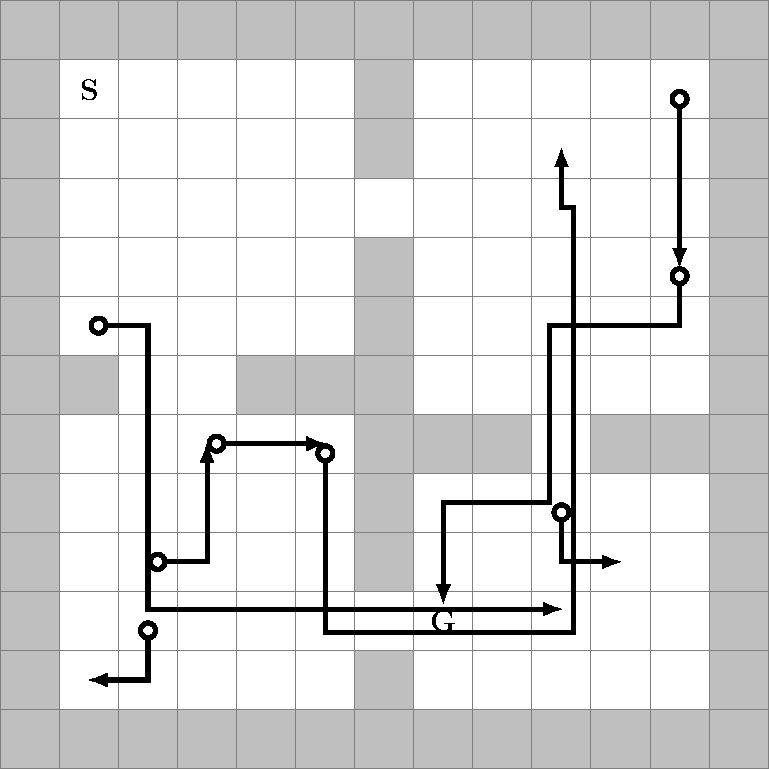
\includegraphics[width=2.4in]{figures/rooms-options}\label{fig:rooms-options}} \hspace{0.25in}
  \subfloat[Rooms: Cumulative Return with 200 options]{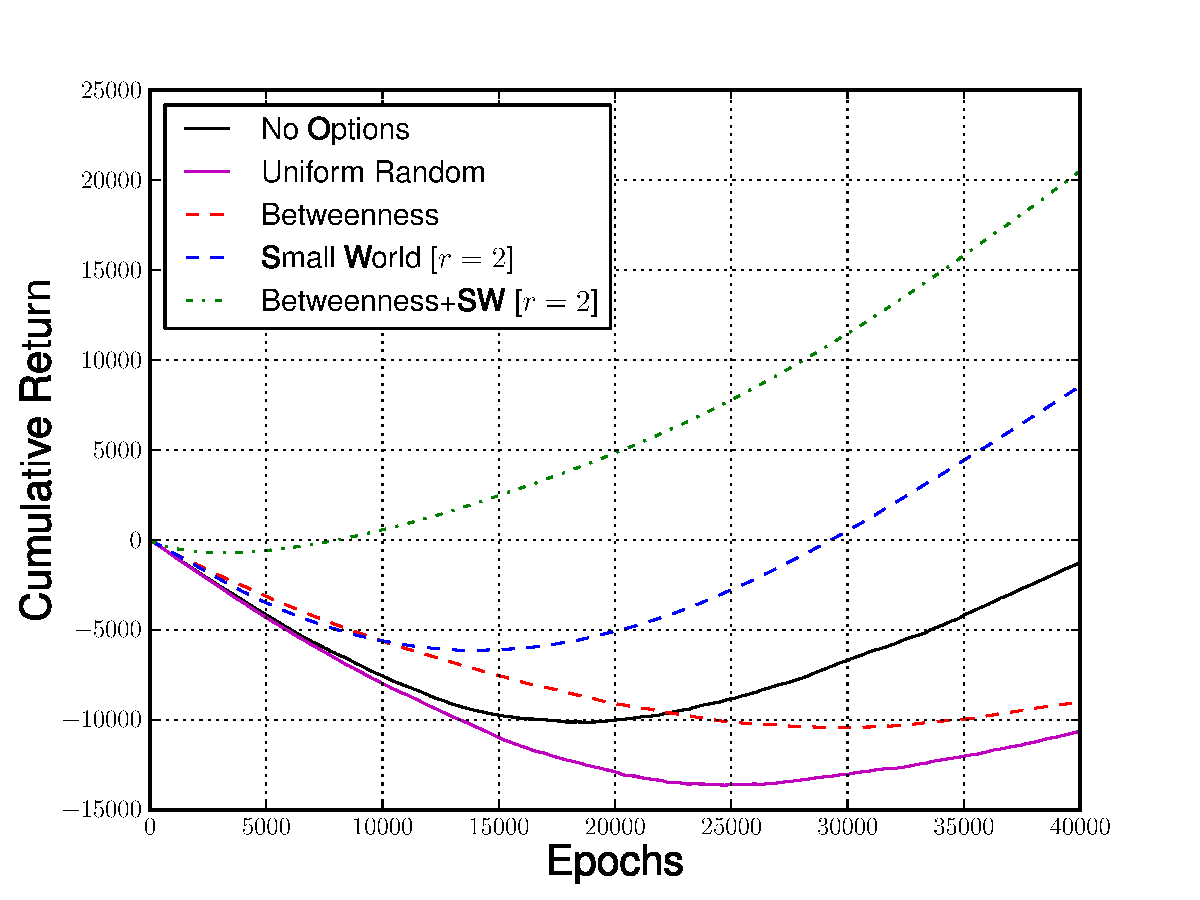
\includegraphics[width=3in]{figures/rooms-return-200}\label{fig:rooms-return}}
\end{figure}

Some of the small world options preferred in Rooms domain are shown in
\figref{fig:rooms-options}. The graph shows several examples of options
that compose together to arrive near the goal state. We have also
plotted the learning behaviour in \figref{fig:rooms-return}. The option
scheme ``Betweenness + SW'' combines options to betweenness maxima with
small world options. Expectedly, it significantly outperforms all other
schemes. The options to betweenness maxima help take the agent between
strongly connected regions, while the small world options help the agent
navigate within the strongly connected region.

\begin{figure}[th]
  \centering
      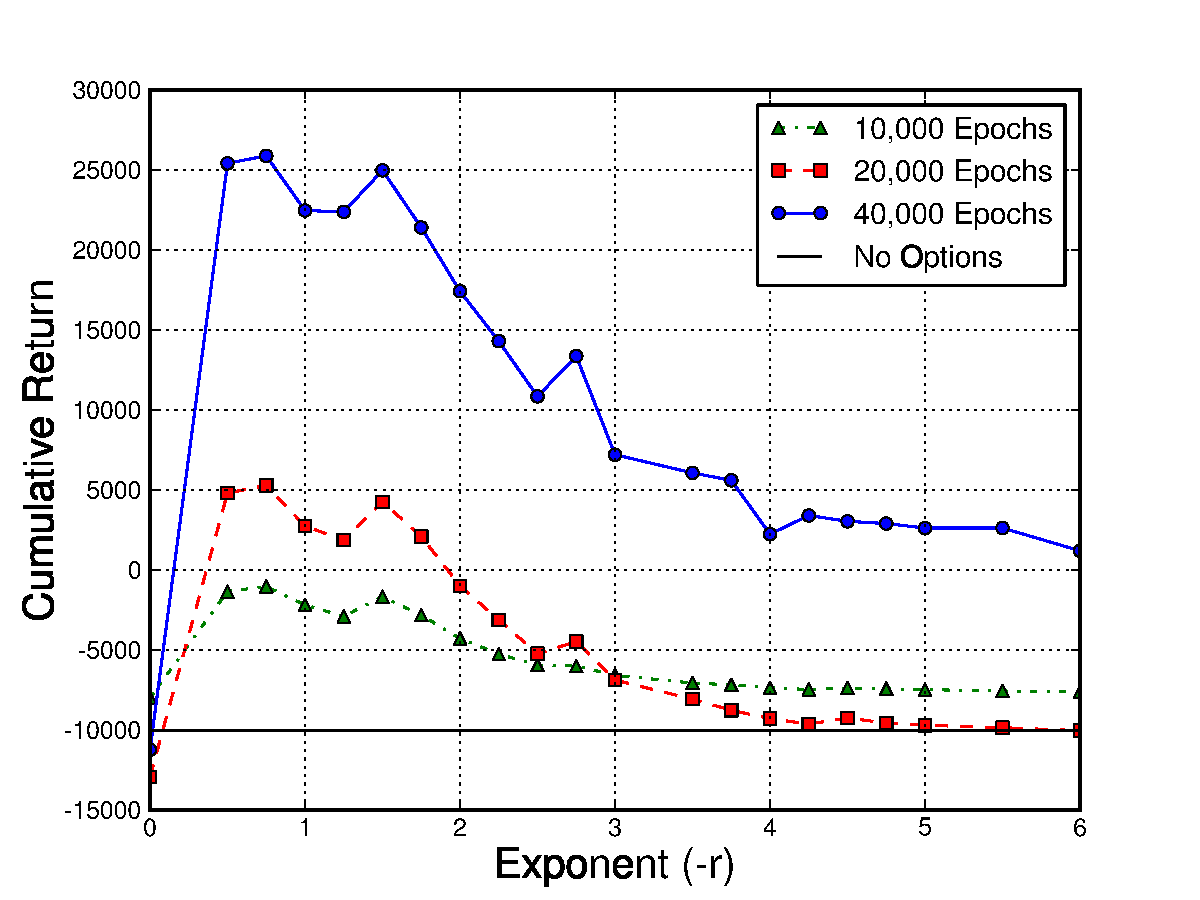
\includegraphics[width=4in]{figures/rooms-exp}
      \caption{Rooms: $r$ vs Cumulative Return}
      \label{fig:rooms-exp}
\end{figure}

\subsection{Sensitivity of $r$}
\label{sec:sw:experiments:sensitivity-r}
\figref{fig:rooms-exp} plots $r$ versus the cumulative return on the
Rooms domain. We do not yet have a clear understanding of how the
exponent $r$ should be chosen. The performance of the agent without
options after $20,000$ epochs is also plotted for reference. There is
a range of $r$ ($\approx 0.75$ to $1.5$) with good performance, after
which the performance steadily drops. This behaviour is easily
explained; as the exponent goes up, the small world options generated
are very short, and do not help the agent get nearer to the maximal
value state. The optimal range of $r$ is slightly counter-intuitive
because the Rooms domain is a two dimensional lattice with some edges
removed. As a consequence of the reduced connectivity, and perhaps due
to stochastic factors, longer range options are preferred.

\begin{figure}[tbh]
  \centering
    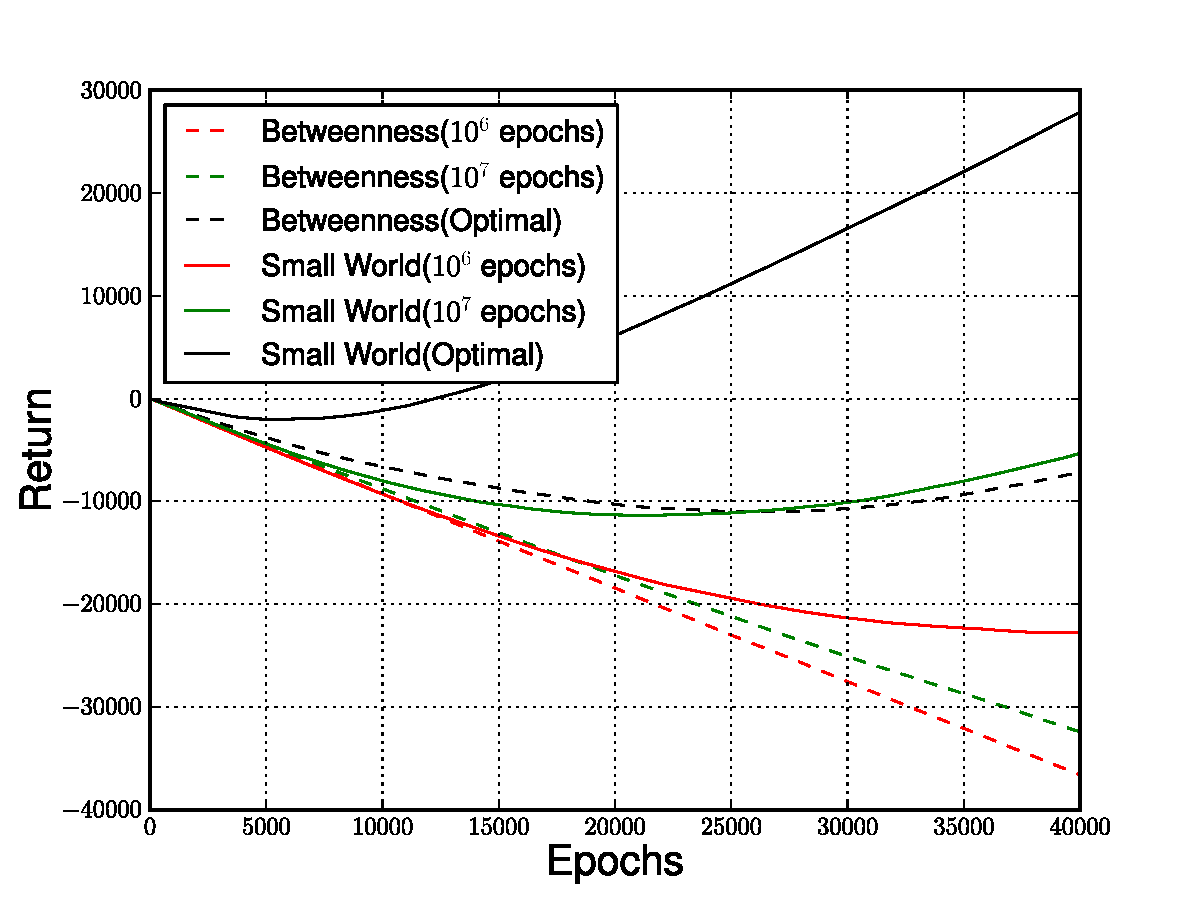
\includegraphics[width=4in]{figures/rooms-learnt-200}
    \caption{Rooms: Options Learnt on a Budget}
    \label{fig:rooms-learnt}
\end{figure}

\subsection{Options Learnt on a Budget}
\label{sec:sw:experiments:budget}
In \secref{sec:sw:algo}, we described an algorithm to construct small
world options efficiently when given a limited number of learning
epochs. We compared the performance of these options with betweenness
options learnt with the same total number of epochs, and have plotted
our results in \figref{fig:rooms-learnt}. Despite using many more
options, the small world options thus created significantly outperform
betweenness options learnt with the same budget, and are even comparable
to the optimal betweenness options.



%\chapter{Conclusions and Future Directions}
\label{chap:conclusions}

\section{Homomorphic Filters}
We described an online algorithm to learn MDP homomorphisms in
continuous state spaces through gradient descent in the family of
homomorphisms, and evaluated the same using the family of affine
homomorphisms. This family of homomorphisms subsumes many existing
selection algorithms which only consider variable remappings. When run
on the Cart Pole domain, the algorithm finds intuitively obvious
approximate homomorphisms which an exact homomorphism solver could not
find. The lifted policy in perturbed domains performs comparably to an
agent trained to learn in that domain. We also used the lifted policy to
bootstrap an agent in the perturbed domain, and observed that the agent
performed better than its counterpart without the lifted policy.

% Experimental results
We believe the homomorphic filter is a novel approach to finding
continuous homomorphisms, backed by a solid theoretical foundation in
MDP homomorphisms. Of particular interest to the authors would be to
study if complex tasks could be solved given models of simpler subtasks.
For example, could we learn how to behave in the Cart Pole domain faster
if we were given a model of an inverted pendulum. This approach
motivates the use of self-paced learning in reinforcement learning.
Though it is straightforward to extend the current work to continuous
action spaces, it remains to be seen how well homomorphic filtering
performs in such domains. Finally, though we have restricted ourselves
to the class of affine homomorphisms, the method described is general
enough to capture other differentiable families, for example regression
trees. Studying alternative homomorphism classes is planned future work.


\section{Small World Options}

% Contributions
% - new scheme for generating options
We have devised a new scheme to generate options based on small world
network model. The options generated satisfy an intuitive criteria, that
the subtasks learnt should be easily composed to solve any other task.
The options greatly improve the connectivity properties of the domain,
without leading to a state space blow up. 

% - absolutely model-free
Experiments run on standard domains show significantly faster learning
rates using small world options. At the same time, we have shown that
learning small world options can be cheaper than learning bottleneck
options, using a natural algorithm that extracts options from a handful
of tasks it has solved. Another advantage of the scheme is that is does
not require a model of the MDP. 

% Further work
% - dynamically add/remove options
% - figuring out r
As future work, we would like to characterise what the exponent $r$
should be in a general domain. There are some technicalities to be
worked out in extending our results to the continuous domain; however,
as most real-life applications are continuous in nature, this is an
important further direction we are looking at.  Given the ease with
which options can be discovered, it would be interesting to experiment
with a dynamic scheme that adds options on the fly, while solving tasks.
\cite{Liben-Nowell2005} extend Kleinberg's results to arbitrary graphs
by using rank instead of lattice distance. It would be interesting to
extend this approach to the reinforcement learning setting. The
logarithmic bounds on the number of decisions presented may have some
interesting consequences on theoretical guarantees of sample complexity
as well.


%\chapter{Publications from this Work}

\begin{enumerate}
  \item Poster at the 9th European Workshop for Reinforcement Learning
    (EWRL 2011), titled ``Learning in a Small World'' described
    preliminary work of \chapterref{chap:sw}.
  \item Full Paper for Oral Presentation at the 11th international
    conference on Autonomous Agents and Multi-agent Systems (AAMAS
    2012), titled ``Learning in a Small World'' described
    the work in \chapterref{chap:sw}.
  \item Paper submitted for review at the 10th European Workshop for
    Reinforcement Learning (EWRL 2012), titled ``Discovering Continuous
    Homomorphisms'' described the work in \chapterref{chap:hf}.
\end{enumerate}



% Chapters-new
%
\chapter{Introduction}
\label{chap:intro}
"Which digital camera should I buy? Which movie should I rent? Which book should I buy for my next vacation?" These are some situations where people have to make decisions about how they are going to spend money, or in a broader level, about their future.
Traditionally, people have used a variety of strategies to solve such decision making problems: conversations with friends, obtaining information from a trusted third party, hiring an expert team or simply follow the crowd. 
%It would be great to have an affordable personal advisor who helps us make good decisions efficiently.
In the present age where e-commerce is flourishing, most e-commerce sites have very large number of products(often in millions) in their databases.
For a user wanting to purchase a product, examining all the products (eg: mobile apps) present in the catalog one after another in the hope of a finding an product that is of interest to him is impractical.
Keyword search is not going to be greatly helpful because an average user does not have a clear understanding of the product space and is often unclear with what kind of products he exactly wants.

We would like to have systems that assist the user to find products of his interest and enable him to efficiently navigate through the complex product space.
\textit{Recommender systems} are constructed for this purpose - assisting a user in his/her (online) decision-making.
%In the present age when e-commerce is flourishing, sizes of product catalogs often is in thousands.
Recommender systems play an extremely important role in matching users to products or items that they might find interesting. 
They filter out huge amounts of information to give personalized suggestions that its users might be interested in. 
This reduces the cognitive effort on the users who are spared of the need to examine a large number of irrelevant items before reaching their desired product.

Recommender Systems are broadly classified into three categories: Collaborative, Content Based and Knowledge Based.

\section{Collaborative Recommender Systems}
\label{sec:CF}
 The main idea in these systems is that if users share the same interests in the past - if they bought or similarly rated the same items - they will also have similar tastes in the future. 
This technique is also called as \textit{Collaborative Filtering}(CF). 
Pure CF based approaches require only rating data and do not require the additional knowledge about underlying users/items. 
Hence, the algorithms are usually domain independent. Most commercial recommender sytems use collaborative filtering for recommending items.
There are two main approaches to perform CF: Memory Based Approaches and Model Based Approaches

\subsection {Memory Based Approaches}
In this approach, the original rating matrix is held in memory and directly used to generate predicted ratings and recommendations. There are two popular memory based approaches:\\
\textbf{User based Nearest Neighbor(NN) Recommendation:} Given a user \textit{u}, the system computes top \textit{K} similar users to \textit{u} according to a pre-defined similarity measure. It recommends those items to user that haven't been rated/purchased by \textit{u} but liked by the top \textit{K} similar users.\\
\textbf{Item based NN Recommendation:} Given a user \textit{u}, the system recommends items that have received similar ratings to the ones that \textit{u} had previously liked.
 


\subsection {Model Based Approaches}
As opposed to memory based approaches that use the ratings matrix to directly generate predictions, model based approaches learn models corresponding to each item and each user from the ratings matrix. The learned models are used to make predictions at run time.
Model based approaches perform well in practice for large datasets.
\textit{Matrix factorization} is a popular model based approach. The superiority of matrix factorization techniques over traditional CF in improving prediciton accuracy was clearly seen during \textit{'The Netflix prize'} competition(\cite{koren}).
Broadly speaking, matrix factorization methods derive a set of latent(hidden) factors from the rating patterns and characterize each item and user as vectors of these factors.
In the movie domain, such latent factors can correspond to some aspects of a movie like genre, but most of them are completely uninterpretable (\cite{koren})


\subsection{Limitations of CF}
\label{sec:limCF}
\textbf{Cold Start Problem:} To provide recommendations for a user \textit{u}, pure CF techniques rely on \textit{u}'s ratings. This means that for a new user who has not yet rated a single item, there is no way of generating personalized recommendations (\textit{new-user problem}). 
Similarly, for a new item that has been recently added to the catalog and has not been rated by a single user, there is no way for it to be recommended to a user (\textit{new-item problem}).\\
\textbf{Sparsity:} The relavance and accuracy of CF recommender's predictions is high when the user-item ratings matrix is dense.
But in real-world systems, the rating matrices are typically very sparse and thus, the quality of recommendations of pure CF approaches may not be good.
As an example, consider a user \textit{u} whose rating pattern is very different from most of the other users. 
He would find it difficult to receive useful recommendations because the number of similar users to \textit{u} is very less(\cite{balab1997}).




%

%

\section{Content based recommender systems}
\label{sec:content}
Collaborative Filtering Systems do not require any knowledge about underlying users/items to make recommendations.
As opposed to this, content based recommender systems rely on item descriptions and explicit/learned user profiles to recommend items.
For example, if the recommender system knows that \textit{Harry Potter} is a fantasy novel and the user Alice has always like fantasy novels, the system can recommend the new \textit{Harry Potter} book right away. 
Content-based recommender systems need not rely on the existence of a large user base to generate recommendations.
It overcomes the cold-start problem described in Section ~\ref{sec:limCF}. However, item characteristics are hard to acquire normally and hence, they have to be entered manually into the system, which can be potentially expensive for some domains (Eg: music).

Having its roots in \textit{Information Retrieval}(IR), content based recommendation most often focuses on textual products - items which can be described in terms of textual features (Eg: documents, news articles and websites).
Most news recommendation systems use content based recommendation to recommend relevant news articles to the users.
A news recommendation system typically recommends news articles by comparing the main keywords of a news article with the keywords in articles that the user has rated highly in the past.
There are two ways in which content based systems can create user-profiles- 
by explicitly asking the user to rate a set of items/topics/categories when the user is new to the system
or by "learning" the user profile automatically by examining the user's past behavior/ratings.
Learning user profiles from user's past behavior can be expensive and sometimes not be accurate because of time-effects(user's interests changing over time) and sparsity of user ratings.
But it has the advantage that it requires no effort from the user.

\subsection{Limitations of Content-based Recommendation}
\textbf{Limited Content Analysis:} Content-based recommender systems perform a shallow content analysis which might not be sufficient in many scenarios. Particularly, for recommending resources such as web pages, aspects other than the keywords like aesthetics, usability and correctness of hyperlinks play a part in establishing the quality of recommendations (\cite{jannach}).
Also, content based recommender systems using limited content analysis based on just keywords, have no way to distinguish between well written and poorly written articles, both of which use the same set of keywords. 
Also, feature extraction techniques for text documents is relatively mature, but the same cannot be said about many multimedia objects like images and videos.
Hence, the usability of content-based recommender systems is limited in multimedia domain. (\cite{adom2005})\\
\\
\textbf{Overspecialization:}  Another drawback of content based recommender systems is that they often tend to recommend items that the user might have already seen/rated. 
A general goal therefore is to increase the serendipity of the recommendation lists - that is, to include "unexpected" items in which the user might be interested in.
The system described by \cite{billsus} therefore defines a threshold to filter out not only items that are too different from the user profile but also those that are too similar.\\
\\
\textbf{New user problem:} The new user problem discussed in Section \ref{sec:limCF} also exists for content based recommender systems.
Although content-based techniques do not require a large user community, they require at least an initial set of ratings from the user, typically a set of explicit \textit{like} and \textit{dislike} statements.
Content-based recommenders do not have the new item problem. 
Given a new item, the recommender system matches the new item's features to existing user profiles and recommends it directly to relevant users.

\section{Knowledge based recommender systems}
Collaborative filtering systems, discussed in Section \ref{sec:CF} suggest items to user based on user's past ratings.
Content based recommender systems, discussed in Section \ref{sec:content} recommend items whose features match the user's profile.
Consider some high-risk product domains like houses, cars, computers etc.
Typically, users do not buy a house, a car or a computer very frequently. 
In such a scenario, both collaborative-filtering or content-based recommender systems may not be able to generate relavant recommendations because of the low number of available ratings.
User-profiles learnt by content-based systems may not be useful for making recommendations due to a heavy influence of time effects(change in user's interests and product catalogs with time). 
For example, if a user has given a high rating to a 'Pentium III' computer four years ago, the recommender system cannot rely on that rating for generating relevant recommendations for the current day.
In complex and high-risk product domains such as computers, customers often want to define their requirements explicitly - for example, "the maximum price of the computer should be $x$ and the hard-disk capacity should be atleast \textit{500GB}".
Knowledge based systems are used to provide recommendations in such scenarios.
%In knowledge based systems, recommendations are made taking into account the explicit user preferences and the rich knowledge base available.

Knowledge-based recommender systems can be divided into two categories: constraint-based and case-based.
Constraint-based recommender systems rely on explicit recommendation rules and case-based recommender systems use similarity/utility measures to generate recommendations. 
A case-based recommendation is typically generated based on similarity of the items in the casebase with the user defined query.
Case-based recommendation and the algorithm for MAUT based recommendation are discussed in detail in Chapter \ref{chap:background}.

Recommendation process of knowledge-based recommender applications is highly interactive, a foundational property that is a reason for their characterization as \textit{\textbf{conversational systems}}. The recommender system that we consider in this project is a conversational recommender system.
Conversational systems assume that a user's initial query is merely a starting point for search, perhaps even an unreliable starting point. The job of a conversational system is to help the user refine his initial preference query as the interactions proceed.
\subsection{Critiquing}
\label{sec:critiquing}

\begin{figure}
\centering
\begin{minipage}{.5\textwidth}
  \centering
  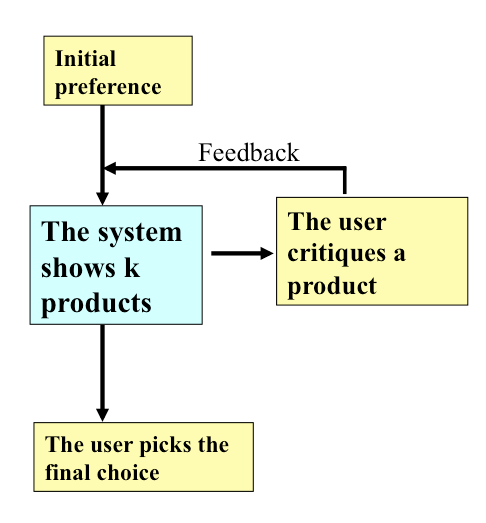
\includegraphics[width=1\linewidth]{figures-bharath/critiquing.png}
  \captionof{figure}{Critiquing}
  \label{fig:critiquing}
\end{minipage}%
\begin{minipage}{.5\textwidth}
  \centering
  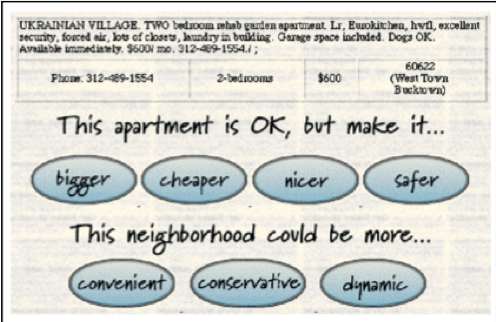
\includegraphics[width=1\linewidth]{figures-bharath/rentMe.png}
  \captionof{figure}{RentMe Recommender System: \cite{burkeRentMe}}
  \label{fig:rentMe}
\end{minipage}
\end{figure}
\textit{\textbf{Critiquing}} is one of the most popular forms of feedback in conversational recommender systems. In each interaction cycle, the user is presented with a list of products.
User selects a product and expresses directional preference(s) over one or more item feature values. 
For example, one might indicate that he is looking for a less expensive restaurant or a more formal setting(Figure \ref{fig:rentMe}). These are two individual critiques, first critique being on the \textit{price} attribute and the second critique on the \textit{setting} attribute. 
The recommender updates it's user model according to this feedback provides another set of products and proceeds to the next recommendation cycle. This continues till the user finally chooses a product. (Figure \ref{fig:critiquing})

\textit{\textbf{Unit critiques}} allow users to express their preference over one attribute in each interaction cycle. \textit{\textbf{Compound critiques}} enable users to input their preferences on several attributes at a time. This can potentially shorten the number of interaction cycles in finding a target product.
The early FindMe Systems \cite{burkeEarlierSystems} had \textit{\textbf{static critiques}}. The critiques wouldn't change when users selected a particular critique. 
This can lead to some serious limitations.
For example, the critique 'cheaper' would continue to be visible, even if there are no cheaper apartments available and when user clicks on 'cheaper', there would be no results displayed at all.
Static critiques also do not represent the best set of tweaks that a user will want to make given his preference model.
The notion of \textit{\textbf{dynamic critiquing}} was first proposed by \cite{mccarthy2004dynamic} to overcome the limitations of static critiques.
Compound critiques are generated on-the-fly for each recommendation cycle. Dynamic critiquing has been shown to improve user-experience and lower the average number of interaction cycles it takes for a customer to find his desired product.

There are two popular approaches to dynamic critiquing: Apriori algorithm based generation of compound critiques (\cite{mccarthy2004dynamic}) and MAUT based generation of compound critiques (\cite{mautPaper}). 
The algorithm for MAUT based recommendation is discussed in Section \ref{sec:maut}.

\subsection{Limitations of Knowledge based recommendation}
Knowledge based recommenders require a high level of knowledge engineering effort.
One needs to define local similarity functions, utility measures, assign weights to features etc.
%Offline evaluation is generally not very reliable in these systems.
%We need to conduct live user studies to prove the efficiency of 

\section{Our contribution: Improvements to MAUT based recommendation}
MAUT based recommendation has been shown (through both user studies and offline experiments) to be one of the best performing recommendation algorithms in the domain of critiquing based recommendation.
Our goal in this project is to improve the performance of MAUT based recommendation.
To this end, we have proposed several algorithms in Chapter \ref{chap:modifications} that led to significant performance improvements.

\section{Organization of the Thesis}
In Chapter \ref{chap:background}, we present an overview of case based recommendation and discuss the algorithms for Apriori and  MAUT based generation of dynamic critiques in detail. We also discuss the offline experiments and live user studies that were conducted to compared the performances of Apriori and MAUT based critiquing.
In Chapter \ref{chap:modifications}, we describe several modifications proposed to MAUT based recommendation algorithm that have led to significant performance improvements.
In Chapter \ref{chap:results}, we describe the experimental procedure and report the the improvements achieved by each of the proposed modifications.
Finally, we present conclusions and possible directions for future work in Chapter \ref{chap:conclusions}.

%\chapter{Background}
\label{chap:background}

% Introduce and summarise this chapter
\section{Reinforcement Learning}
\label{sec:background:rl}

In reinforcement learning, the standard representation of an
environment and task instance is a Markov decision process (MDP). An
MDP can be represented as the tuple, $\tuple{ \states, \actions,
\transitions, \rewards, \gamma }$, where $\states$ and $\actions$ are
the state and action domains which are known to the agent.
$\transitions: \states \times \actions \to \measure(\states)$, where
$\measure(\states)$ is the set of all probability measures over
$\states$, describes the dynamics of the world through state-action
transition probabilities. $\rewards: \states \times \actions \to \Re$
describes the task at hand by ascribing rewards for state transitions.
Both $\transitions$ and $\rewards$ are initially unknown to the agent.
Finally, $\gamma \in [0,1)$ is a parameter, called the `discount
factor', that weighs the value of future rewards. 

\begin{figure}[ht]
  \centering
  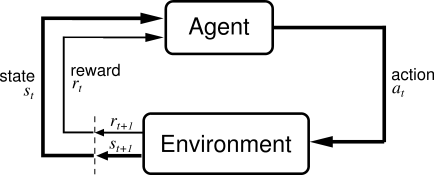
\includegraphics[width=3in]{figures/agent-environment.png}
  \caption{Agent-Environment Interface}
  \label{fig:agent-env}
\end{figure}

% Figure here
In this setting, an agent in a state $s \in \states$ chooses an action
$a \in \actions$, and moves to a state $s'$ with probability
$\transitions(s'|s,a)$, receiving a reward $\rewards(s,a)$
(\autoref{fig:agent-env}). In the fully observable setting, the agent is
aware of which state it is in, and the objective of the agent is to find
a policy $\policy: \states \to \measure( \actions )$, i.e. a decision
procedure for selecting actions, that maximises the reward it
accumulates in the long run, $R = \sum_{i} \gamma^i r_i$. $R$ is also
called the return. 

In the remainder of this section, we will describe the basic approach
for finding an optimal policy $\policy$ for a discrete MDP, and its
continuous variant. 

% Various representations of MDPs

% Discrete MDPs
\subsection{Discrete Markov Decision Processes}
 
In the discrete case, $\states$ and $\actions$ are predictably finite
sets of states and actions. We define the value function $V^{\pi}:
\states \to \Re = \E_{\pi}[\sum_{t=0}^{\infty} \gamma^{t} R_t | S_0
= s ]$ to be the expected return from $s$, and $Q^{\pi}: \states \times
\actions \to \Re = \E_{\pi}[\sum_{t=0}^{\infty} \gamma^{t} R_t | S_0
= s, A_0 = a ]$ to be the expected return from $s$, after taking the
action $a$. These can be written in a recursive form,
\begin{eqnarray*}
  V^{\pi}(s) &=& \max_{a} \rewards(s,a) + \gamma \sum_{s' \in \states} \transitions(s'|s,a) V^{\pi}(s') \\
  Q^{\pi}(s,a) &=& \rewards(s,a) + \gamma \sum_{s' \in \states} \transitions(s'|s,a) Q^{\pi}(s',a').
\end{eqnarray*}

Our objective can then be stated as finding a policy $\pi$ with an
optimal value function, i.e. $V^{*}(s) = \sup_{\pi} V^{\pi}(s)$ at all
$s \in \states$. The optimal value functions must satisfy the Bellman
optimality conditions, 
\begin{eqnarray*}
  V^{*}(s) &=& \max_{a} \rewards(s,a) + \gamma \sum_{s' \in \states} \transitions(s'|s, a) V^{*}(s') \\
  Q^{*}(s,a) &=& \rewards(s,a) + \gamma \sum_{s' \in \states} \transitions(s'|s,a) \max_{a'} Q^{*}(s',a').
\end{eqnarray*}

Given an optimal $Q$, it is possible to construct a greedy policy that
is optimal; $\pi(s,a^*) = 1$ when $a^* = \argmax_{a} Q(s,a)$, and $0$
otherwise. In principle, if the agent knew the MDP, it could construct
the optimal value function, and from it an optimal policy.  However,
in the typical setting, the agent is only aware of the state-action
space, $\states$ and $\actions$, and must learn $Q$ through
exploration. The Q-learning algorithm learns $Q$ with a simple update
for every step the agent takes, $$Q(s,a) = Q(s,a) + \alpha
[ r + \gamma \max_{a'} Q(s',a') - Q(s,a) ],$$ where $\alpha \in [0,1]$
is a parameter that controls the learning rate.  It has been shown
that the Q-learning algorithm converges to the optimal value function
in the limit with fairly permissive assumptions.

% Continuous MDPs
\subsection{Continuous Markov Decision Processes} 

In continuous domains, defining $\states$ and $\actions$ must be done
with some care. To begin with, $\states$ must be a measurable
Euclidean space \footnote{Roughly, a space $X$ is said to be
measurable if a monotonic function $\mu: 2^X \to \Re$ that is additive
over finite union can be defined.}; let us denote the Lebesgue measure
\footnote{The Lebesgue measure is a generalisation of length/area. It
is possible to construct a Lebesgue measure for any Euclidean space.}
by $\lambda$.  Consider the following (mild) regularity assumption
proposed in \citet{Andra2008}, 
\begin{property}(MDP Regularity)
  \label{prop:mdp-regularity}
  $\states$ is a compact subset of the $d_{\states}$-dimensional
  Euclidean space, $\actions$ is a compact subset of $[-A_{\infty},
  A_{\infty}]^{d_{\actions}}$. The random immediate rewards are bounded
  by $\hat{R}_{\max}$ and $\rewards$ is uniformly bounded by $R_{\max}:
  \|r\|_{\infty} \le R_{\max}$.
\end{property}

We define the evaluation operator; $T^{\pi}:B(\states \times \actions)
\to B(\states \times \actions)$, $$ T^{\pi}Q(s,a) = \rewards(s,a)
+ \gamma \int_{\states,\actions} \ud s' \ud a'~ \transitions(\ud
s'|s,a) \pi(a'|s') Q(s',a').  $$ We now define the analogue of the
$Q$-value function recurrence relation, $Q^{\pi} = T^{\pi}Q^{\pi}$.
The fixed point of the Bellman operator $T :B(\states \times \actions)
\to B(\states \times \actions)$, $$ TQ(s,a) = \rewards(s,a) + \gamma
\int_{\states} \ud s'~ \sup_{a' \in \actions} \transitions(\ud s'|s,a)
Q(s',a'),$$ $Q^* = TQ^*$ is then the optimal value function. By the
regularity conditions imposed in \autoref{prop:mdp-regularity},
$V^{\pi}$ and $Q^{\pi}$ are both bounded by $\frac{R_{\max}}{1
- \gamma}$.

In order to approach learning an optimal policy, we must estimate the
current value function, $Q$. One method is to use a function
approximator. Another popular scheme is the Fitted Q-iteration
approach, wherein the $Q$ function is estimated by regressing on
a finite trajectory collected using a stationary policy $\pi_b$. Let
$[S_t, A_t, R_t]_{1 \le t \le N}$, be the dataset, and then $Q_{k+1}$
can be got by, $$Q_{k+1} = \textrm{Regress}( \left\{ [(S_t, A_t), R_t
+ \gamma \max_{a' \in \actions} Q_k(X_{t+1},a')]_{1 \le t \le N-1}
\right\} ).$$

The regression itself can be solved using a variety of methods,
including neural networks and SVMs. A further discussion on suitable
regression methods, and a proof of convergence subject to niceness
assumptions can be found in \citet{Andra2008}.

\section{Spatial Abstractions: Homomorphisms}
\label{sec:background:homs}

% TODO: Clean up.
A homomorphism is defined in general to be a structure-preserving map.
In the context of MDPs, we want a correspondence between the two
systems' dynamics ($\transitions$) and tasks ($\rewards$). 

\begin{definition}(MDP Homomorphism)
An MDP homomorphisms $h$ from an MDP $\mdp = \tuple{S,A,P,R,\gamma}$ to
and MDP $\mdp' = \tuple{S',A',P',R',\gamma}$ is a surjection for the
state-action spaces $S \times A \to S' \times A'$ such that,
\begin{eqnarray}
  P'(h(s,a),\him{s'}) &=& \sum_{s' \in \finv{f}(\him{s'})} P(s,a,s') \label{condition:hom-P} \\
  R'(h(s,a)) &=& R(s,a), \label{condition:hom-R} 
\end{eqnarray}
\noindent
where $f$ is $h$ restricted to $S$, i.e. $f(s) = h(s,a)\mid_S$, and
$\him{s'}$ is the image of $s'$ in $\mdp'$, i.e. $\him{s'} = f(s')$.
\end{definition}

With minor abuse of notation, we assume $P(h(s,a),\him{s'}) \triangleq
P(\him{s}, \him{a}, \him{s'})$, where $h(s,a) = (\him{s}, \him{a})$.
Similarly, $Q(h(s,a)) = Q(\him{s},\him{a})$. For brevity, we will write
$\mdp \hom{h} \mdp'$ if $\mdp'$ is the homomorphic image of $\mdp$ under
$h$. We will also use the notation $(s,a) \in \mdp$ to mean $(s,a) \in
S \times A$. Finally, two state-action pairs $(s,a)$ and $(s',a')$ are
equivalent if $h(s,a) = h(s,a') = (\him{s},\him{a})$. We write this as
$(s,a) \sim (s',a')$.

There can be other, less strict definitions of homomorphisms based on
preserving the value function, policy behaviour, etc. A survey of these
definitions can be found in \cite{Li06}.

% Description of major problems for homomorphisms.
Given this definition, there are perhaps four serious questions that
we wish to answer when talking about homomorphisms,
\begin{enumerate}
  \item (Transfer) Given a homomorphisms $g$ between MDPs $M$ and $M'$,
    can one use a policy learnt in $M$ in $M'$, and vice versa?
  \item (Discovery) Given MDPs $M$ and $M'$, are they homomorphic? 
  \item (Minimisation) Given an MDP $M$, what is the smallest $M'$
    isomorphic to $M$?
  \item (Approximate Minimisation) Given an MDP $M$, and a class of
    homomorphisms $H$, what is the closest approximation $M' \in H(M)$
    of $M$?
\end{enumerate}

All of these questions have been convincingly answered in the case of
discrete MDPs. 

% Description of how homomorphisms can be used to pull back policies 
\subsection{Transferring Policies in Discrete MDPs}

The primary application of MDP homomorphisms is in the transfer of
learning in problem to another. 

\begin{definition}(Lifted Policy)
  Given $\mdp \hom{h} \mdp'$, and a policy $\pi'$ in $\mdp'$ we can
  define a {\em lifted policy} $\pi = \finv{h}(\pi')$ in $\mdp$ as
  follows,
  \begin{eqnarray}
    \pi(s,a) &\triangleq& \frac{\pi'(h(s,a))}{ |\{a':h(s,a') = h(s,a)\}| }. \\
             &=& \frac{\pi'(h(s,a))}{ |\{a':(s,a') \sim (s,a)\}| }.
  \end{eqnarray}

  Note that the denominator equally distributes the selection
  probability between equivalent actions for a state.
\end{definition}

A powerful result that we will later review shows that the lifted
policy of an optimal policy is itself optimal. This is a special case
of the result that the value of the lifted policy is equal through out
$M$ to the value of the original policy in $M'$, i.e. for all $s$,
$V^{\pi}(s) = V^{\pi'}(\him{s})$.

% Description of how homomorphisms can be used in context of relativized options.
\begin{note}(Partial Homomorphisms and Relativised Options)

  \begin{figure}[ht]
    \centering
    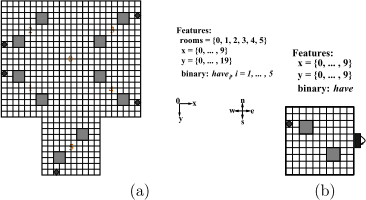
\includegraphics[width=3in]{figures/relativized-options.png}
    \caption{Relativised Options}
    \label{fig:relativised-options}
  \end{figure}

The ability to `lift' policies from one MDP to another can be exploited to
solve subproblems in a reinforcement learning domain. Consider the grid-world
shown in \autoref{fig:relativised-options}(a) taken from \cite{Ravindran2003};
in this domain, there are several rotated copies of the room shown in
\autoref{fig:relativised-options}(b). For each room in (a), let us define a
homomorphism mapping each cell within the room to those of the template room
(b). All states outside the room are mapped to the `sink' state, denoted by the
black square in (b). We can now define {\em options}
\cite{SuttonPrecupSingh1999} for each room, using the optimal policy for (b),
$\pi$, and the above homomorphisms; $\options = \{\finv{h_r}\pi(a) \mid \mbox{for
each room $r$} \}$.

\end{note}

\section{Temporal Abstractions: The Options Framework}
\label{sec:background:options}

The options framework provides a temporal abstraction through subtasks.
An option $\option$ is described by an initiation set $\initset \subset
\states$, a policy $\pi$, and a terminating condition $\beta$.  An agent
can exercise an option in any state $s \in \initset$, following which,
it will follow the policy $\pi$ described by the option, until the
terminating condition $\beta(s)$ is satisfied. The terminating condition
$\beta$ can be stochastic.

Several learning algorithms have been proposed for agents using options
\cite{SuttonPrecupSingh1999,BartoMahadevan2003}. One simple such method that
we will use is MacroQ, a generalisation of the Q-learning algorithm
described above. The MacroQ algorithm updates the value function only
after completion of the option. If the option $o$ was initiated in the
state $s$, and continues for $k$ steps before terminating in $s'$, the
corresponding $Q$ function update will be,
\begin{eqnarray*}
    Q(s,o) &=& Q(s,o) + \alpha [ r + \gamma^{k} \max_{o' \in \actions \cup \options} Q(s',o') - Q(s,o) ].
\end{eqnarray*}

Different tasks in the same domain can be described by different
$\rewards$. Let $\rewards$ be sampled from the family $\Rewards$. Our
objective then is to find a set of options $O$ that reduces the expected
learning time over $\Rewards$.

\begin{example}
  \label{example:taxi}

\begin{figure}[th]
    \centering
    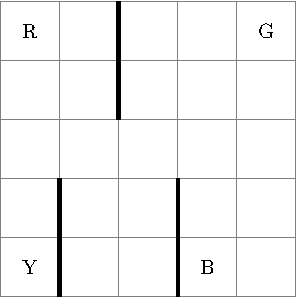
\includegraphics{figures/taxi}
    \caption{The Taxi Domain}
    \label{fig:taxi-domain}
\end{figure}
To make the discussion more tangible, let us look at an example, the
Taxi domain, shown in \figref{fig:taxi-domain}. The agent is a taxi
navigating in this road-map. It must pick up a passenger at one of the
4 pads, R, G, B or Y.  Subsequently, it must carry the passenger to a
destination, which is also one of the above four pads. The states of
the taxi would then be a tuple containing the location of the
passenger (in one of the four pads, or within the taxi), the
destination of the passenger, and location of the taxi in the map.
The actions the taxi can perform are moving up, down, left or right in
the map, as well as pick up or drop a passenger at a pad. 
Typical options for such a domain would be an option that can be
started anywhere, and has a policy that takes the taxi to the one of
the pads in the shortest possible manner. Such an option is generic,
and does not depend on where the passenger or destination are. The RL
agent must then learn to choose the right option when picking up the
passenger.
\end{example}

\section{Small World Networks}
\label{sec:background:sw}

\begin{figure}[ht]
  \centering
  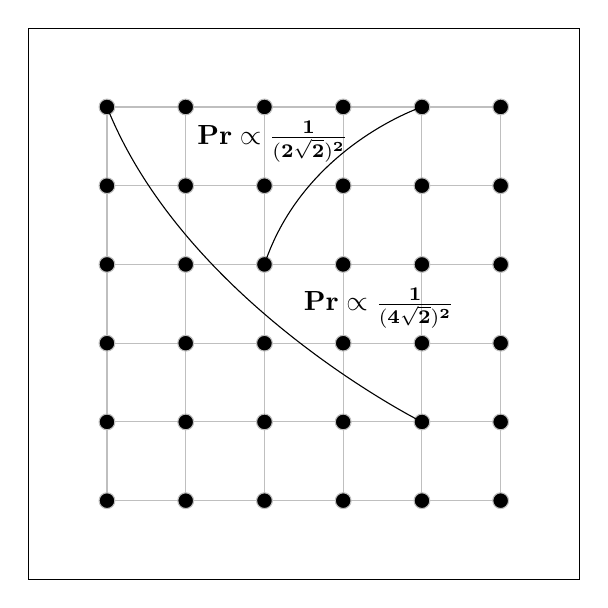
\begin{tikzpicture}[]
    % Grid
    \draw[clip] (-1,-1) rectangle (6,6);
    \draw[step=1,color=lightgray] (0,0) grid (5,5);
    \foreach \xpos in {0, 1, 2, 3, 4, 5}
    {
      \foreach \ypos in {0, 1, 2, 3, 4, 5}
      {
      \draw [color=lightgray,fill=black,opacity=1.0] (\xpos,\ypos) circle (0.1);
      };
    };

    % Draw some long range edges
   \draw (2,3)  .. controls (2.5,4.5) and (4,5) .. node [left] {$\mathbf{Pr \propto \frac{1}{(2\sqrt{2})^2}}$} (4,5);
   \draw (0,5)  .. controls (1.0,2.5) and (4,1) ..  node [above right] {$\mathbf{Pr \propto \frac{1}{(4\sqrt{2})^2}}$} (4,1);

\end{tikzpicture}
  \caption{Kleinberg's Small World Network}
  \label{fig:kleinberg-sw}
\end{figure}

% What are small world options
In Kleinberg's small-world network model (\figref{fig:kleinberg-sw}),
each node $u$ is given one `long-range' edge to a node $v$, which was
chosen with a probability $P_r(u,v) \propto \|u-v\|^{-r}$, where
$\|u-v\|$ denotes the least distance between nodes $u$ and $v$ in the
graph. On an $r$-dimensional lattice, $\klein_r$, the distance from
any node $u$ to a target node $t$ is bounded by $\|u-t\|$, a quantity
which is locally computable. When given long-range edges distributed
according to $P_r$, \citet{Kleinberg2000} showed that a greedy
distributed algorithm $\greedyalgo$ that chooses a neighbour $v$
closest to $t$ will reach $t$ with an expected time $O(\log(|V|)^2)$.
This result is significant because the expected time for the algorithm
on a graph with edges distributed uniformly, i.e. without dependence
on distance, is $O(|V|^2)$.

\begin{theorem}
  \label{thm:kleinberg-sw}
  Let $f: V \to \Re$ be a vertex function, and $M_f$ be the global
  maxima of $f$. Consider an algorithm, \greedyalgo, that greedily
  chooses the neighbour with the highest value of $f$. Suppose the
  algorithm is currently at $u$, it will choose $N(u) = \argmin_v \|f(v)
  - f(M_f)\|$.
  
  If $\graph(V,E)$ is $r$-dimensional lattice, and contains a long
  distance edge distributed according to $P_r: p(u,v) \propto
  \|u-v\|^{-r}$, then \greedyalgo takes $O( (\log |V|)^2 )$ steps to
  reach $M_f$.
\end{theorem}
\begin{proof}
  We defer the proof of this theorem to \secref{sec:sw:theory}, where we
  prove a generalisation of this theorem (\thmref{thm:sw}).
\end{proof}


%\chapter{Modifications to MAUT Based Generation of compound critiques}
\label{chap:modifications}
\section{Limitations of MAUT Based Critiquing:}

We have seen in Sections \ref{sec:offline} and \ref{sec:liveUser} that MAUT based recommendation performs slightly better than Apriori algorithm in offline experiments and live user studies.
However, there are several limitations to MAUT based recommendation, which when addressed can improve it's performance significantly.
The limitations to MAUT based recommendation are as follows:
\begin{itemize}
\item Critique strings in a given iteration can be very similar to each other. This doesn't give the user too many options to choose from.
\item Preference model is updated only based on the most recently selected product. History of user selected products/critique strings is not considered while updating the preference model.
\item Top five products shown in the first cycle is same for all user-queries
\item In a particular recommendation cycle, if all the critique strings have "Higher Price", user is forced to select a critique string with "Higher Price". We would ideally not want to update the weight of the attribute $price$, since we cannot infer whether user is willing to compromise on $price$ attribute. But MAUT based recommendation algorithm will actually decrease the weight of $price$ attribute by a factor of $\beta$.
\item As an extension to the above point, Consider the case when there are 4 critique strings with "Lower Resolution" and 1 critique string with "Higher Resolution". If the user selects the critique string that has "Higher Resolution", we can update  the weight of 'Resolution' attribute by a higher factor.
\item The fact that a particular product has been preferred over the remaining (k-1) rejected products is not exploited

\end{itemize}
%put section numbers when all the description is done...
We try to address the above each of the above limitations in Sections (Numbers) and also propose some additional improvements that improve the performance of MAUT based recommendation.


\section{Diversity in Critiques}

A variant of \textit{\textbf{Bounded Greedy Selection}} algorithm described in \cite{boundedGreedy} was used to generate diverse critiques in every cycle.
The function \textit{GenCritiqueItems(PM, IS)} is modified as follows:\\
\\

\begin{algorithm}[ht]
  \SetKwInOut{Input}{input}\SetKwInOut{Output}{output}
  \DontPrintSemicolon
  %\Input{$PM$, $IS$}

  $R \gets \{\}$\\
  $CB' \gets IS$\\
  \For{ $i\gets0$ \KwTo $k$ }{
    Sort $CB'$ by $Quality(i, R, PM)$ for each case in IS; \\
    $R \gets R + First(CB')$;\\
    $CB' \gets CB' - First(CB')$;\\
  }
  \Return R
  \caption{GenCritiqueItems(PM, IS)}
  \label{algo:div}
\end{algorithm}

\begin{algorithm}[ht]
  \SetKwInOut{Input}{input}\SetKwInOut{Output}{output}
  \DontPrintSemicolon
  %\Input{$i$, $R$, $PM$}

  \If {$R == \{\}$} {return 0;}
  \Else {
      $retVal \gets \alpha \times utility(i, PM)$; \\
      $disSim \gets \frac{\sum_{r_j \in R} (1-critiqueSim(i,r_j))}{|R|}$;\\
      $retVal += (1-\alpha) \times disSim$;\\
      $return retVal$;\\
  }
  \Return retVal
  \caption{Quality(i, R, PM)}
  \label{algo:quality}
\end{algorithm}

$critiqueSim(a, b)$ returns the extent of overlap between the individual attribute directions of products $a$ and $b$.
We get the best results when $\alpha = 0.5$.
Introducing diverse critiques in every cycle results in significant improvement in the number of interaction cycles and it also improves user experience (Users don't prefer critiques being very similar to each other).


\begin{figure}
\centering
\begin{minipage}{.45\textwidth}
  \centering
  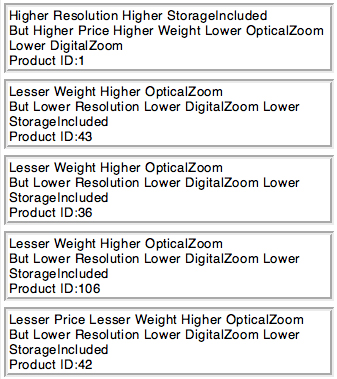
\includegraphics[width=1\linewidth]{figures-bharath/diversity1.jpg}
  \caption{Before diversifying critique strings}
  \label{fig:beforeDiv}
\end{minipage}%
\;\;\;\;\;\;
\begin{minipage}{.45\textwidth}
  \centering
  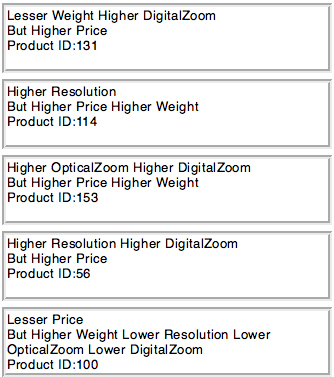
\includegraphics[width=1\linewidth]{figures-bharath/diversity2.jpg}
  \caption{After diversification}
  \label{fig:afterDiv}
\end{minipage}
\end{figure}



\section{Selectively updating value functions of nominal attributes}
As seen in Section \ref{sec:valueFunc}, the value of $\gamma$ used to update the value functions of nominal attributes is constant in each cycle.
Instead, we propose an alternative approach in which the value of $\gamma$ varies according to the number of alternatives the user rejected while choosing a particular attribute value. 
Stronger the preference the user has for a particular attribute value, higher is the value of $\gamma$.
The intuition for varying the value of $\gamma$ is as follows: Consider the case when there are five PCs displayed to the user and the manufacturers of the five PCs are "Compaq", "HP", "Apple", "Dell" and "Toshiba".
If the user selects the PC with "Compaq" as the manufacturer, we can see that he has accepted "Compaq" and rejected four other manufacturers.
Thus, we can say that the user has a strong preference for "Compaq" PCs.
On the other hand, in the case when all the five PCs have a screen size of 15 inches and the user selects the PC with screen-size of 15 inches, we cannot really infer whether the user has a strong preference for 15 inch PCs.
Generalizing the examples above, if $k$ is the value of the attribute N selected in a cycle and $R$ is the list of values of attribute $N$ of the top-K products other than the selected products, we define
%
\begin{equation}
\gamma = \frac{\#\: of\: alternatives\: to\: k\: in\: R}{|R|}
\end{equation}
%
If attribute $N$ = "Manufacturer"; $\gamma$ = 1 when manufacturer of all the remaining products is different from the selected product's manufacturer($M$) and also different from each other; meaning that the user has a strong preference for $M$.
$\gamma$ = 0 when manufacturer of all remaining products is same as the selected product's manufacturer($M$).
This is the case when we cannot infer whether the user has a strong preference for $M$.
This is similar to weighted MLT described in \cite{comparisonbr}.
Some examples of how the value of $\gamma$ varies are illustrated in Table \ref{tab:wMLT}
Varying the value of $\gamma$ according to the other products' attribute values results in a significant improvement in the number of interaction cycles.



\begin{table}
\renewcommand{\arraystretch}{1.5}
 \centering
 \begin{tabular}{l l l l l l |l|}
  \hline \hline
   Feature & P1 & P2 & P3 & P4 & P5 & $\gamma$ \\
  \hline
  Manufacturer & Dell & Apple & Compaq & HP & Toshiba & 1.0 \\
  Type & Laptop & Laptop & Laptop & Laptop & Laptop & 0 \\
  Processor & Core-i3 & AMD-E1 & Core-i7 & AMD-E1 & Core-i3 & 0.5\\
  Screen-size & 15 & 13.3 & 15 & 15 & 15 & 0.25\\
  \hline \hline
 \end{tabular}
 \caption{Values of $\gamma$ when P3 is selected by the user}
 \label{tab:wMLT}
\end{table}


\section{Varying the level of diversity}
\label{sec:div2}
In Section \ref{sec:div}, we have discussed a method of introducing diversity in every cycle.
We know that, at the beginning of a recommendation session, an average user does not have a good understanding of the product space and trade-offs that exist between different product attributes.
But after interacting with the recommender system for a few cycles, he develops a good understanding of the product space and his preferences become more stable.
Therefore, it is a good idea to introduce diversity in the beginning of a recommendation session so that user will develop a better understanding of the product space and then show targeted recommendations after a few cycles when his preferences have stabilized.

We propose a new approach where diversity is varied adaptively according to whether user's preferences have stabilized.
Consider an attribute 'Price'.
If the maximum difference between prices of previous $K$(=3) products selected by the user is less than a pre-defined threshold, we assume that the user is satisfied with this particular product price and we promote cases that have a price closer to the average price of the $K$ products in the next cycle.
%Consdiering camera dataset, if the difference between 'weight' of each of the previous $K$(=3) selected products is less than a certain threshold,
If the maximum difference between the weights of the previous $K$(=3) products is greater than the pre-defined threshold, we assume that user's preference for the 'weight' attribute has not stabilized yet. 
Hence, we try to display products that are diverse to each other in terms of 'weight' attribute.
The numeric attributes for which we assume that user's preference has stabilized are classified into the set $simA$.
The other numeric attributes are classified into the set $divA$.
In the implementation, the function \textit{GenCritiqueItems(PM, IS)} is the same as described in Algorithm \ref{algo:div}.
The function \textit{Quality(p, R, PM)} is modified as follows:

\begin{algorithm}[ht]
  \SetKwInOut{Input}{input}\SetKwInOut{Output}{output}
  \DontPrintSemicolon
  %\Input{$i$, $R$, $PM$}

  $ret \gets \alpha \times utility(i, PM)$; \\
  $simA, divA$ = classifyAttributes(); \\
  $avg$ = previousKProductAttributeAverages(); \\
  $tmp \gets 0$;\\
  \For{ each attribute $x_i$ in $simA$ }{
      $tmp$ += (sim($avg(x_i)$, $p(x_i)$));\\
  }
  \For{ each attribute $x_i$ in $divA$ }{
      $tmp += \frac{\sum_{r_j \in R} (1-sim(p(x_i),r_j(x_i)))}{|R|}$;\\
  }

  $tmp = (1-\alpha) \times \frac{tmp} {\lvert simA\rvert + \lvert divA\rvert}$\\
  \Return $ret + tmp$ ;\\
  \caption{Quality(p, R, PM)}
  \label{algo:quality2}
\end{algorithm}

We will refer to the algorithm described in this section as \textbf{DIV2} in the subsequent sections.




%\chapter{Experimental Results}
\label{chap:results}
\section{Experimental Methodology}


%Add the introduction sentence, we compare so-and-so with standard MAUT
We use two standard datasets, \textbf{Camera} and \textbf{PC}, in our experiments.
Both the datasets are available for download at \cite{datasets}.
Cases with missing values have been removed from the datasets.
After removing the cases with missing values, the Camera dataset contains 173 cameras with 10 attributes and the PC dataset contains 120 PCs with 8 attributes.
A typical PC in the PC dataset is shown in Table \ref{tab:pc} and a typical camera in the Camera dataset is shown in Table \ref{tab:camera}.


\begin{table}
\caption{A typical PC in the PC dataset}
\centering
\renewcommand{\arraystretch}{1.2}
\label{tab:pc}

\begin{tabular}{|l|l|}
\hline
Manufacturer & Apple \\
\hline
Processor Type & PowerPC G3 \\
\hline
Processor Speed(MHz) & 600 \\
\hline
Monitor (Inches) & 15 \\
\hline
Type & Laptop \\ 
\hline
RAM (MB) & 512 \\
\hline
Drive Capacity(GB) & 40 \\
\hline
Price (\$) & 986\\
\hline
\end{tabular}
\end{table}

\begin{table}
\caption{A typical camera in the Camera dataset}
\centering
\renewcommand{\arraystretch}{1.2}
\label{tab:camera}

\begin{tabular}{|l|l|}
\hline
Manufacturer & Sony \\
\hline
Model & DSC-T11 \\
\hline
Price(\$) & 383\\
\hline
Format & Ultra-compact\\
\hline
Resolution (MP)  &5\\
\hline
Optical Zoom (X) &3 \\
\hline
Digital Zoom (X) &4\\
\hline
Weight (grams) &230\\
\hline
Storage Type & Memory Stick\\
\hline
Storage Included (MB)& 32\\
\hline
\end{tabular}
\end{table}

To evaluate the algorithms in offline setting, we simulate an artificial user who interacts with the recommender system.
A product is first selected from the case base and a random subset of it's features is used to formulate the simulated user's query at the beginning of the recommendation session.
This product is now the target for the recommender system and the recommendation session terminates when this product appears in the list of $K$ products shown to the user. 
Subsets of 1, 3 and 5 features are referred to as Q1, Q3 and Q5 respectively.
Queries in Q1 category correspond to users who have very limited domain knowledge.
Queries in Q5 category correspond to users who have a very clear idea about what products they exactly want.
For both PC and Camera datasets, we generate queries of the type Q1, Q3 and Q5.
The same set of queries has been used for all the experiments done below.
Each product in the case-base is set as the target product 10 times and this is repeated for all products in the case-base.
Hence a total of 1730 and 1200 queries for each of the three categories Q1, Q3 and Q5 have been generated for Camera and PC datasets respectively.
The evaluation of all the algorithms described in Sections \ref{sec:div} to \ref{sec:additive} are performed in two scenarios described in Section \ref{sec:focus} and \ref{sec:noisy}, where the artifical user interacts with the system in two different ways.
The complete implementation for all the algorithms described in Sections \ref{sec:div} to \ref{sec:additive} is available at 
%\url{https://github.com/abharath27/MAUTNew}.
\cite{implementation}.

\section{Highly Focused Recommendation Framework}
\label{sec:focus}
Evaluation in Highly Focused Recommendation Framework is the same way of evaluation described in Section \ref{sec:offline}.
In this scenario we assume that the user is relatively sure of his preferences and hence chooses the critique string that is maximally compatible with the target product in each cycle.
The notion of selecting the most compatible critique string is shown in Figure \ref{fig:focus}

%This will help  us to illustrate the noisy framework better.
\begin{figure}[h]
  \centering
  \captionsetup{justification=centering}
    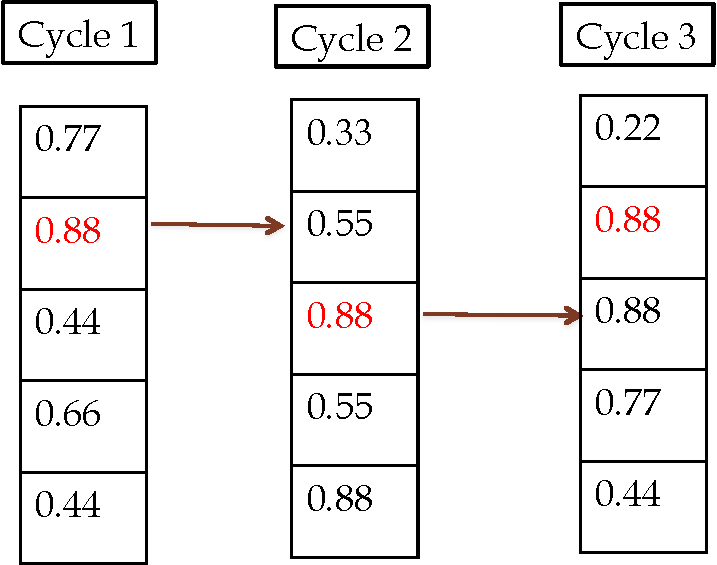
\includegraphics[width=0.5\textwidth]{figures-bharath/focus.pdf}
  \caption{Numbers in the boxes represent the compatibilities of each of the five critique strings with the target product. Simulated user selects the most compatible critique string (red) in each cycle.}
\label{fig:focus}
\end{figure}

\begin{figure}[h]
  \centering
  \captionsetup{justification=centering}
    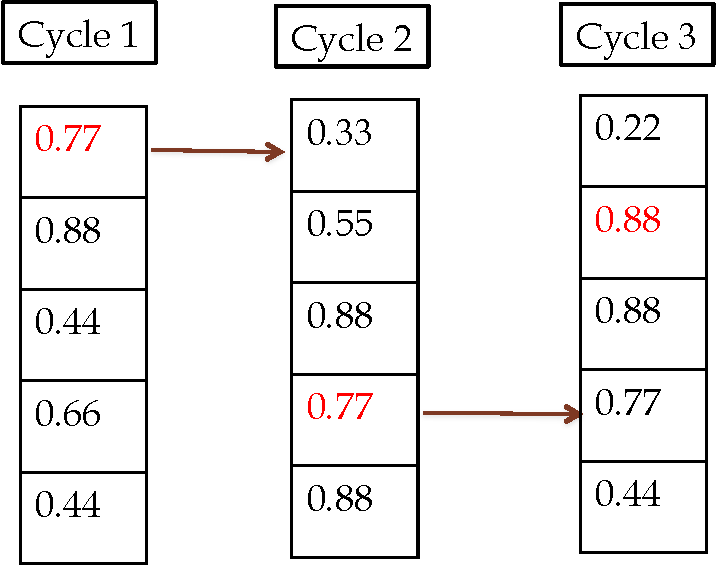
\includegraphics[width=0.5\textwidth]{figures-bharath/noisy.pdf}
  \caption{Simulated user selects sub-optimal critique strings due to the introduction of noise}
\label{fig:noisy}
\end{figure}

\section{Noisy Framework}
\label{sec:noisy}
In this scenario, the simulated user does not select the most optimal critique string during each cycle.
This kind of evaluation is similar to the evaluation procedure described in \cite{suggestion}.
Noise is introduced into the process by varying the compatibility scores of the critique strings within some threshold. 
In our experiments, we have used a noise level of 10\%, i.e, the compatiblity scores can be changed by upto +/-10\% of their actual values.
Due to the introduction of noise, the uesr makes sub-optimal choices in each cycle as shown in Figure \ref{fig:noisy}.
In the experiments, the simulated user selects a sub-optimal critique string for 28\% times on an average in noisy setting.
The average number of interaction cycles in this scenario is slightly higher in this scenario compared to the number of cycles in highly focused recommendation framework because of sub-optimal choices made by the simulated user.


\section{Results}
\subsection{Diversity enhancing algorithms}
\label{sec:div_results}
The algorithm described in Section \ref{sec:div} (abbreivated as DIV), introduces diversity among critique strings in every cycle. 
The algorithm described in Section \ref{sec:div2} (abbreivated as DIV2), introuduces diversity according to the extent to which the user's preferences have stabilized.
The results for the algorithms DIV and DIV2 in both optimal and noisy settings for PC and Camera datasets are summarized in the Figures \ref{fig:div_camera_opt} to \ref{fig:div_pc_noisy}.
For the queries of category Q1 on the in Figure \ref{fig:div_camera_opt}, the implementation of standard MAUT based recommendation takes 9.21 cycles on an average to reach a target product.
DIV and DIV2 take 7.82 and 6.82 cycles on an average to reach the target product.
DIV and DIV2 achieve a reduction of 22.6\% and 27.8\% respectively in the average number of cycles.
The average number of cycles in MAUT is 10.35 in noisy setting, which is 12\% higher than the number of cycles in noisy setting.



\begin{figure}[h]
\centering
\begin{minipage}{.45\textwidth}
  \centering
  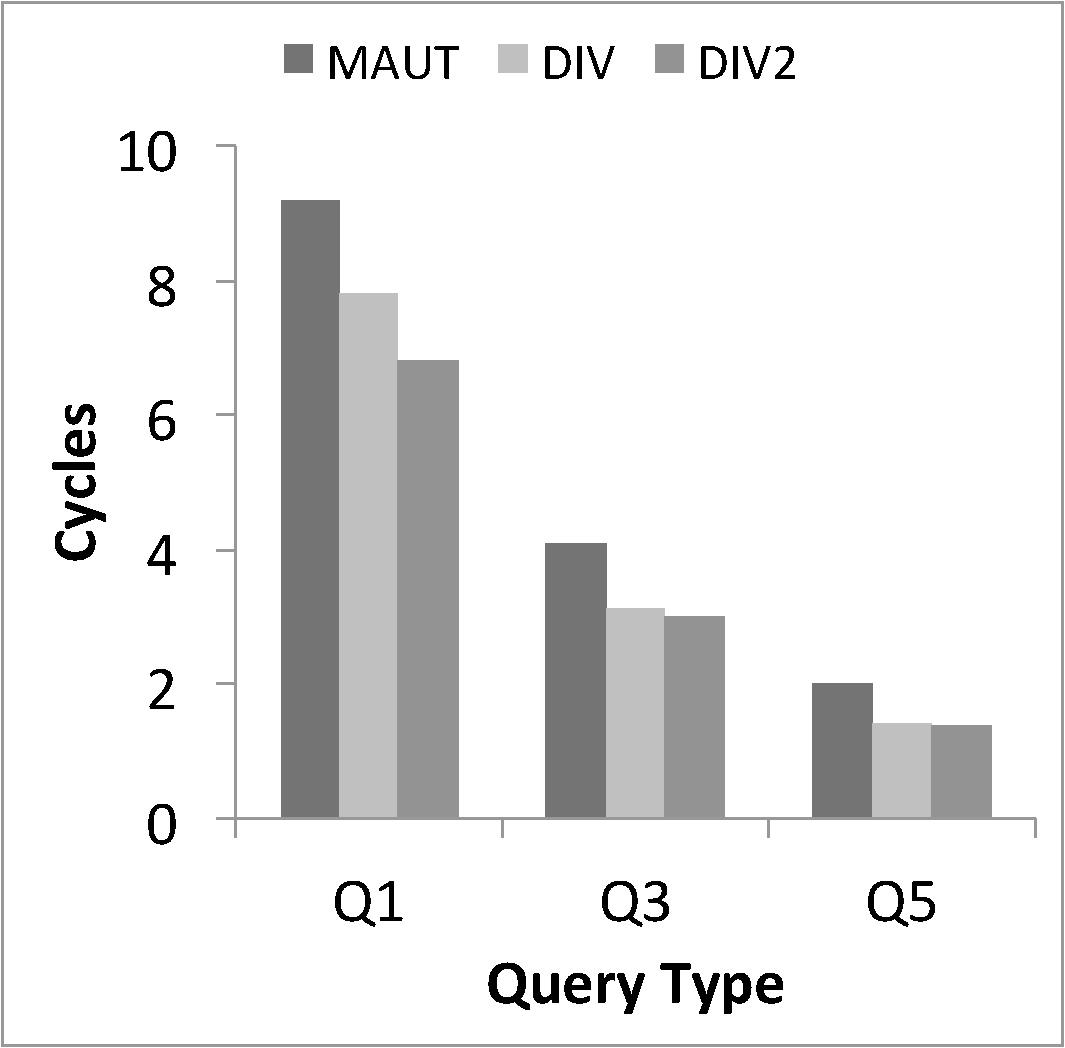
\includegraphics[width=1\linewidth]{figures-bharath/div_camera_opt}
  \caption[]{Average number of interaction cycles on Camera dataset - optimal user model}
  \label{fig:div_camera_opt}
\end{minipage}%
\;\;\;\;\;\;
\begin{minipage}{.45\textwidth}
  \centering
  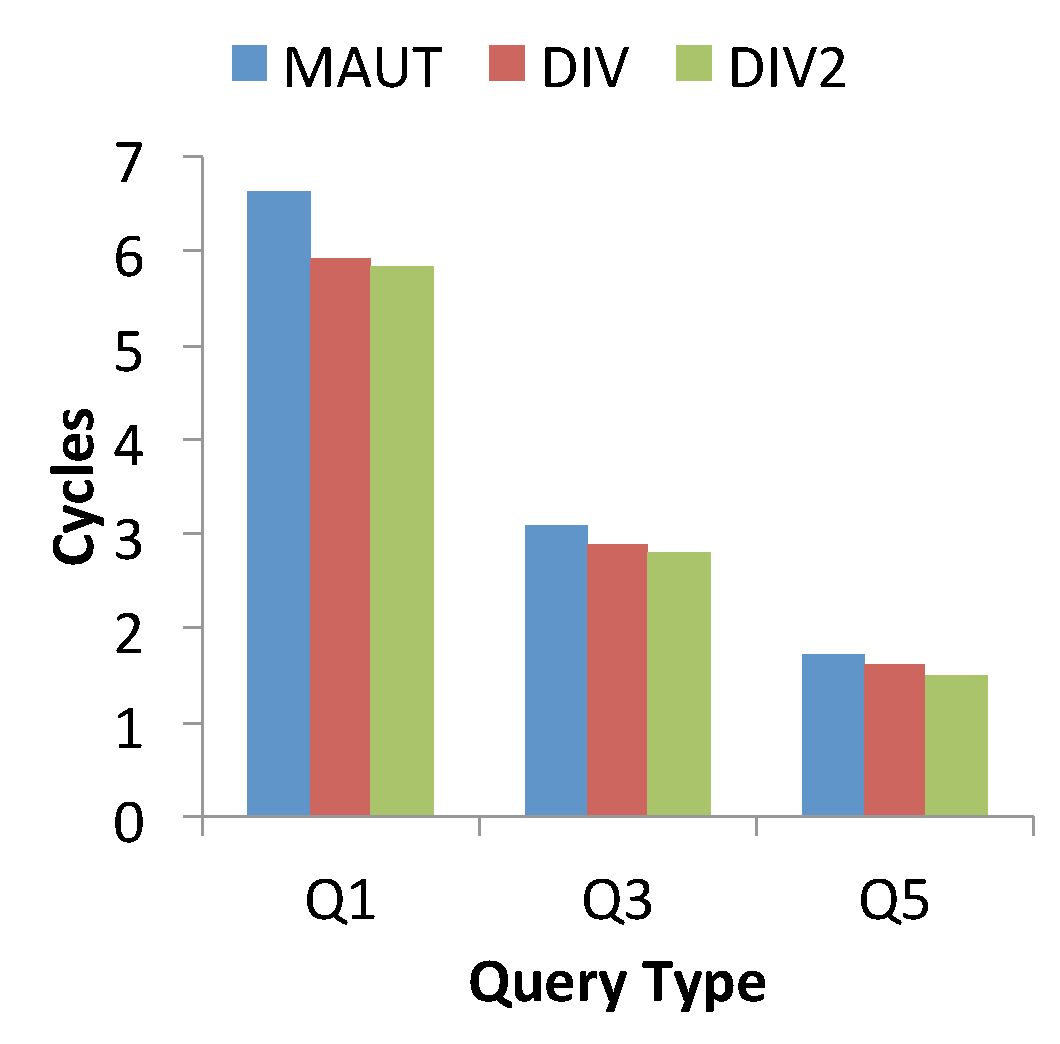
\includegraphics[width=1\linewidth]{figures-bharath/div_pc_opt}
  \caption[]{Average number of interaction cycles on PC dataset - optimal user model}
  \label{fig:div_pc_opt}
\end{minipage}
\end{figure}

\begin{figure}[h]
\centering
\begin{minipage}{.45\textwidth}
  \centering
  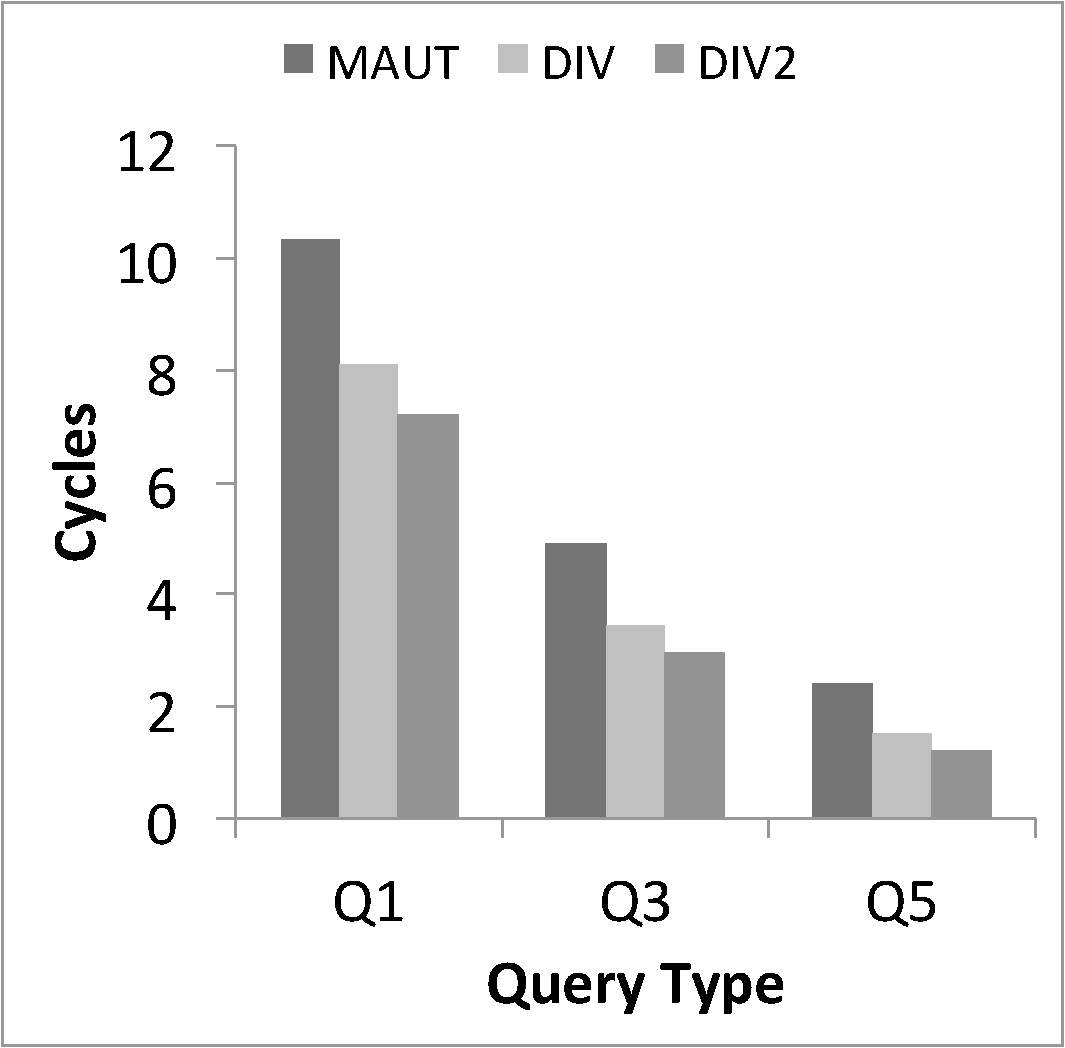
\includegraphics[width=1\linewidth]{figures-bharath/div_camera_noisy}
  \caption[]{Average number of interaction cycles on Camera dataset - noisy framework}
  \label{fig:div_camera_noisy}
\end{minipage}%
\;\;\;\;\;\;
\begin{minipage}{.45\textwidth}
  \centering
  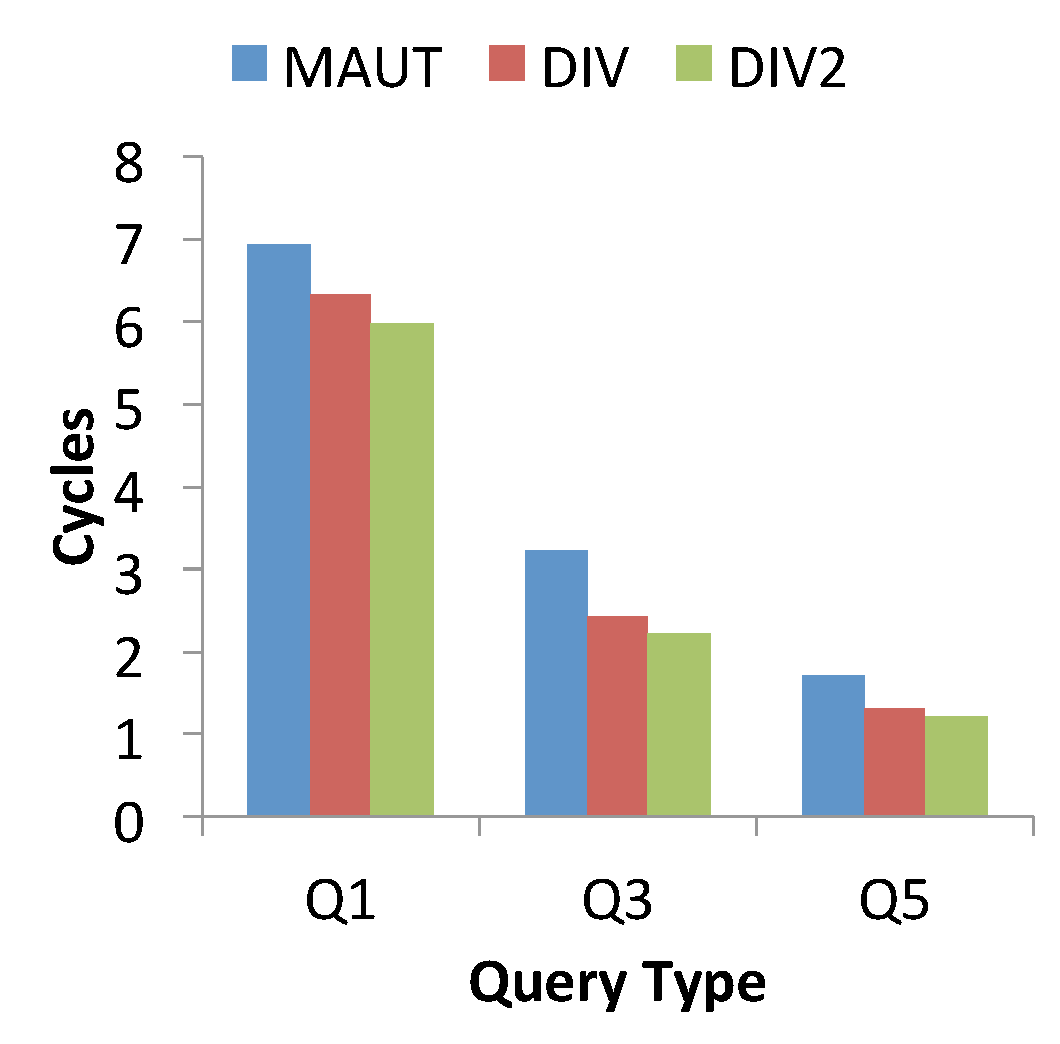
\includegraphics[width=1\linewidth]{figures-bharath/div_pc_noisy}
  \caption[]{Average number of interaction cycles on PC dataset - noisy framework}
  \label{fig:div_pc_noisy}
\end{minipage}
\end{figure}

\subsection{Algorithms that combine similarity with utility}
In Algorithm \ref{algo:addPref} (ADDPREF), we have promoted products that have a critique pattern similar to the product selected by the user in previous cycle.
In Algorithm \ref{algo:addPref2} (ADDPREF2), an extension to ADDPREF, we consider critique overlap of a product with all the products that have been selected so far.
The performance for both the algorithms are shown in Figures \ref{fig:addPref_camera_opt} to \ref{fig:addPref_pc_noisy}.
In highly focused recommendation framework, ADDPREF and ADDPREF2 give an average improvement of 31.1\% and 33.8\% respectively.

\begin{figure}[h]
\centering
\begin{minipage}{.45\textwidth}
  \centering
  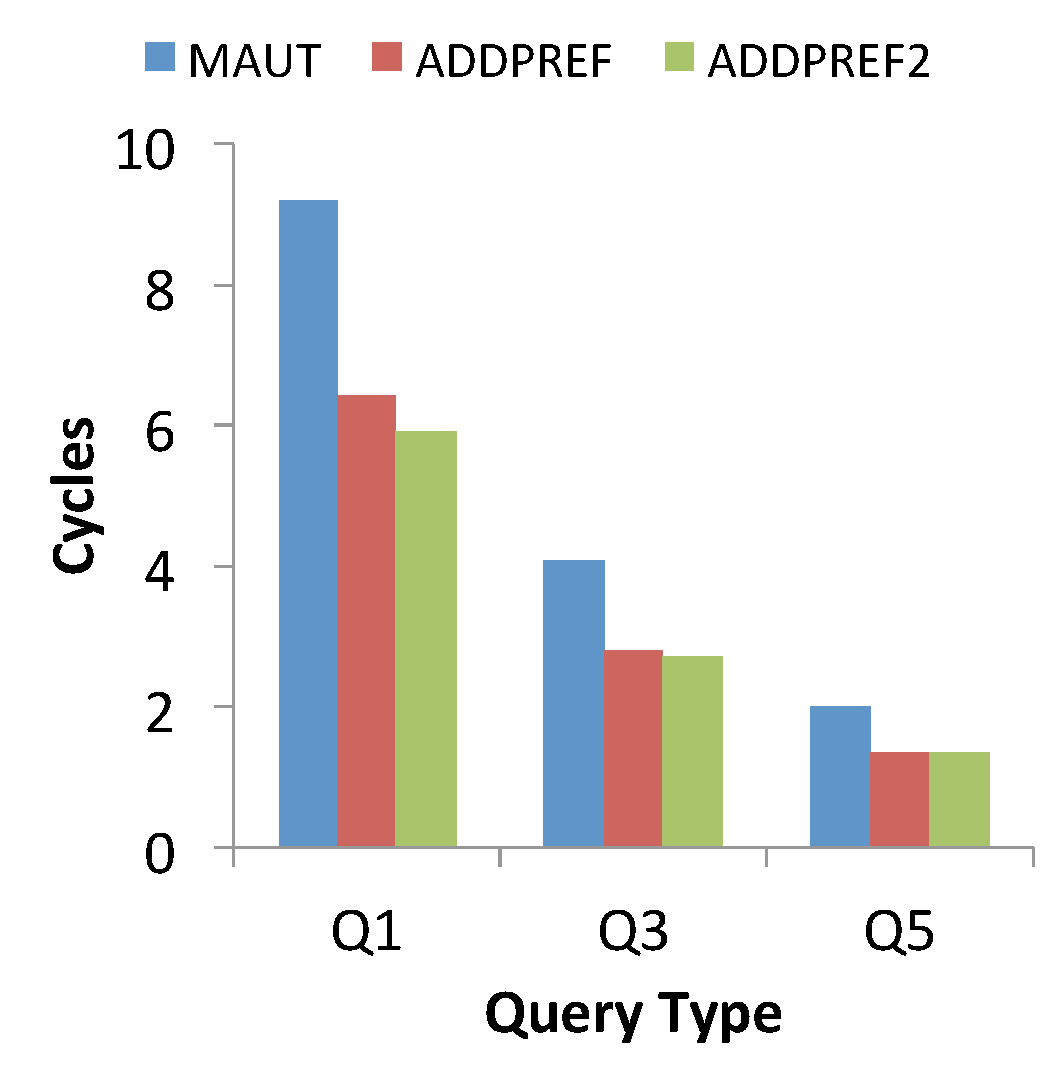
\includegraphics[width=1\linewidth]{figures-bharath/addPref_camera_opt}
  \caption[]{Average number of interaction cycles on Camera dataset - optimal user model}
  \label{fig:addPref_camera_opt}
\end{minipage}%
\;\;\;\;\;\;
\begin{minipage}{.45\textwidth}
  \centering
  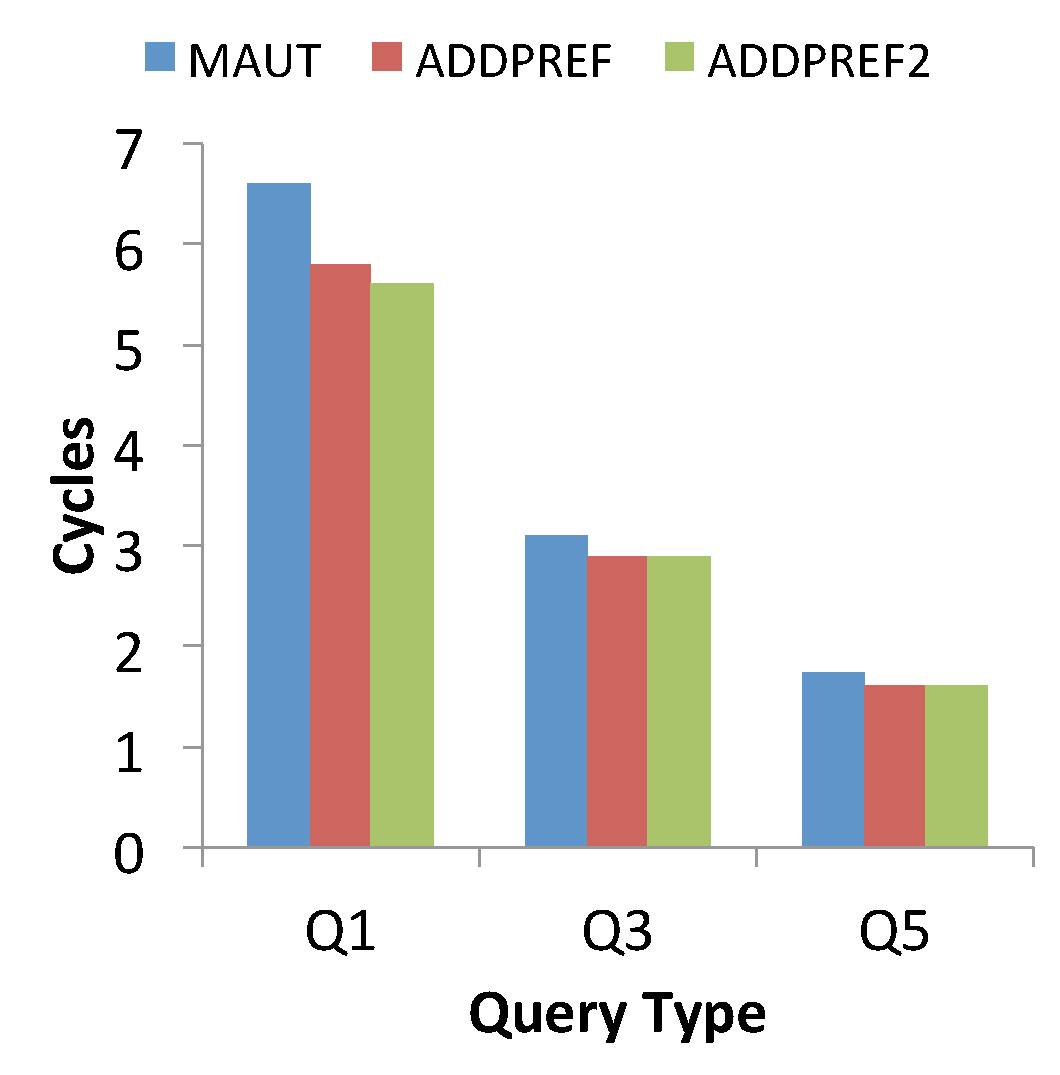
\includegraphics[width=1\linewidth]{figures-bharath/addPref_pc_opt}
  \caption[]{Average number of interaction cycles on PC dataset - optimal user model}
  \label{fig:addPref_pc_opt}
\end{minipage}
\end{figure}

\begin{figure}[h]
\centering
\begin{minipage}{.45\textwidth}
  \centering
  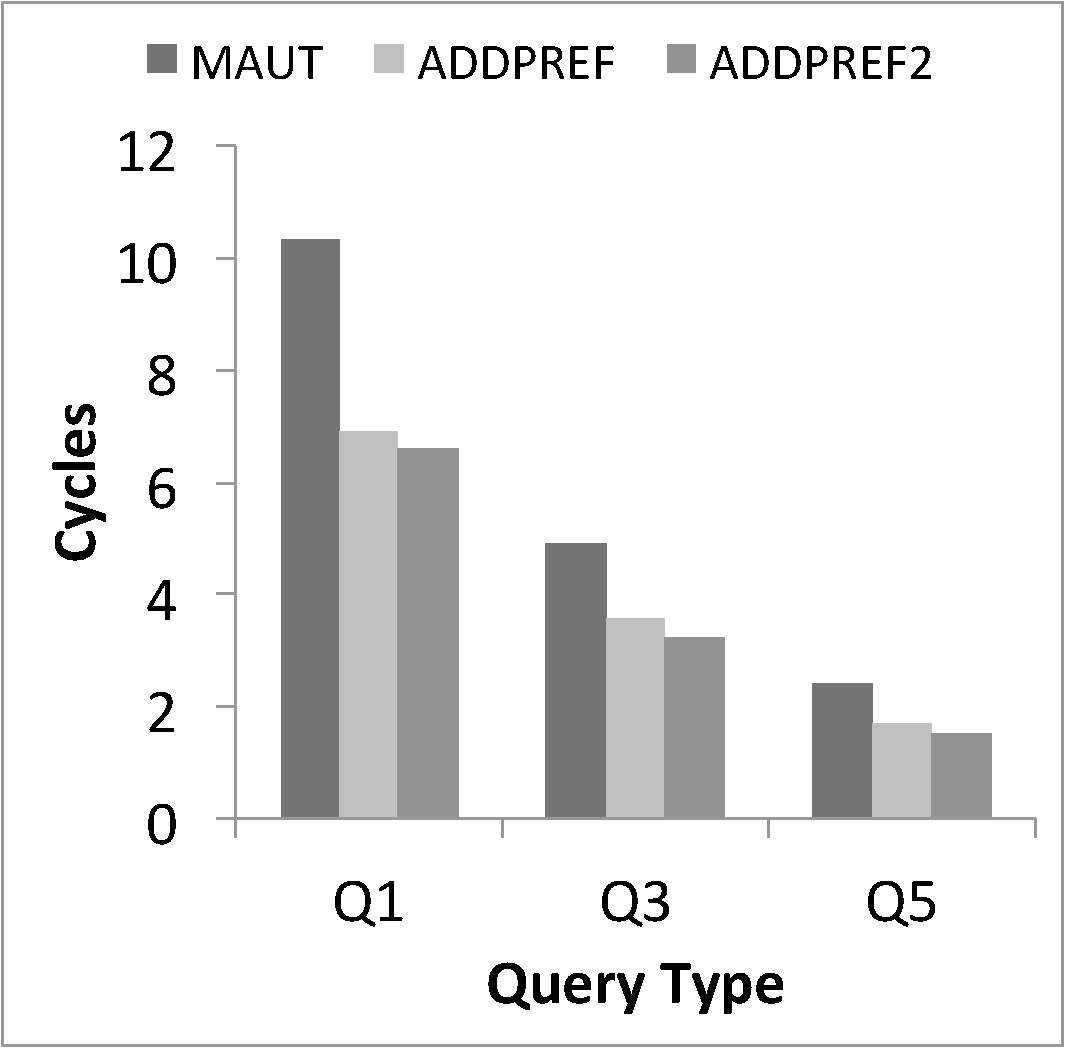
\includegraphics[width=1\linewidth]{figures-bharath/addPref_camera_noisy}
  \caption[]{Average number of interaction cycles on Camera dataset - noisy framework}
  \label{fig:addPref_camera_noisy}
\end{minipage}%
\;\;\;\;\;\;
\begin{minipage}{.45\textwidth}
  \centering
  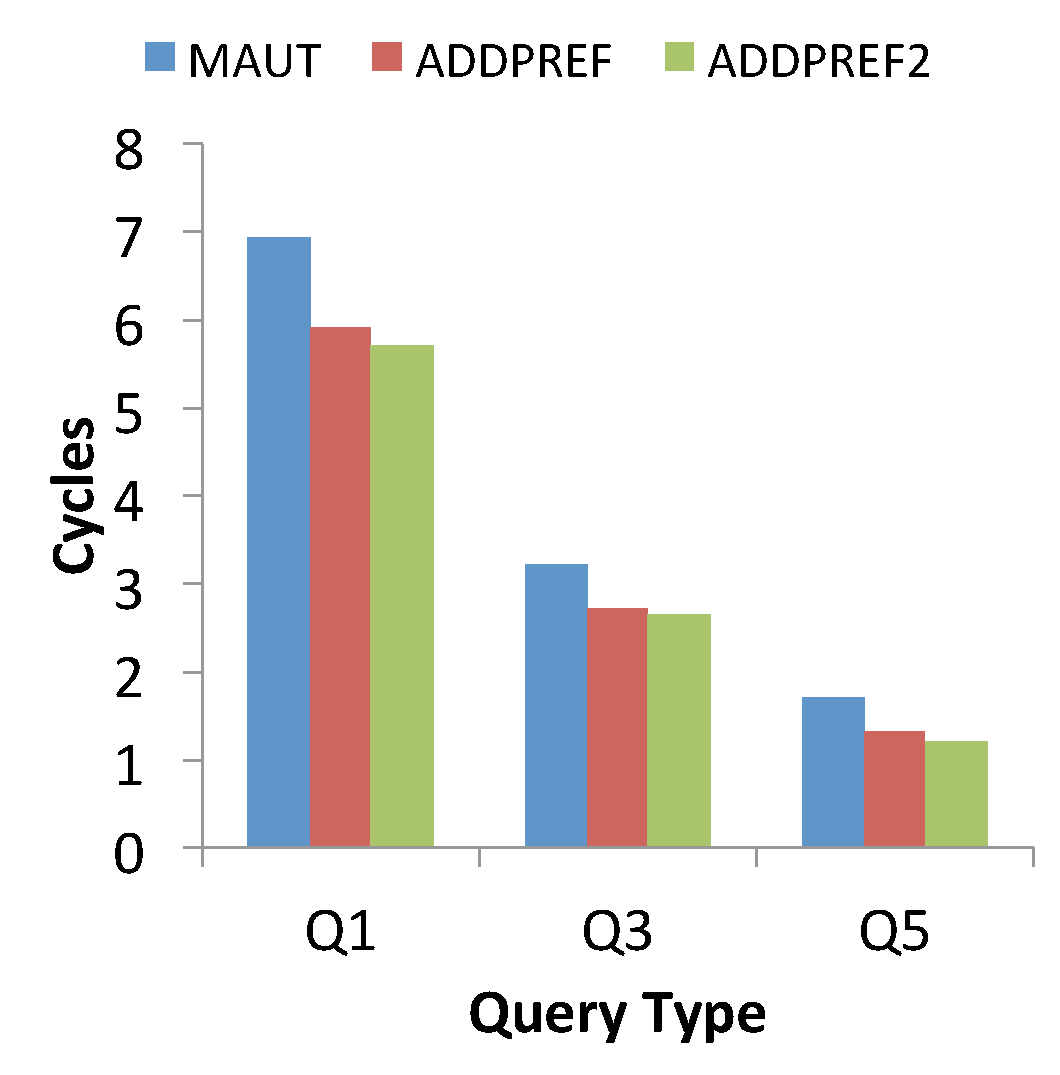
\includegraphics[width=1\linewidth]{figures-bharath/addPref_pc_noisy}
  \caption[]{Average number of interaction cycles on PC dataset - noisy framework}
  \label{fig:addPref_pc_noisy}
\end{minipage}
\end{figure}

In Section \ref{sec:sim}, we have proposed a modification(SIM) where we introduce the products that are most similar to user's initial query.
This simple modification actually produces a very high improvement in the number of interaction cycles.
SIM reduces the average number of cycles by 32.6\% on an average.
SIM when combined with ADDPREF2, reduces the average number of cycles even further. 
The reduction is 40.3\% on average in this case.
The results obtained in the two scenarios for Camera and PC datasets have been shown in Figures \ref{fig:sim_camera_opt} to \ref{fig:sim_pc_noisy}.

\begin{figure}[h]
\centering
\begin{minipage}{.45\textwidth}
  \centering
  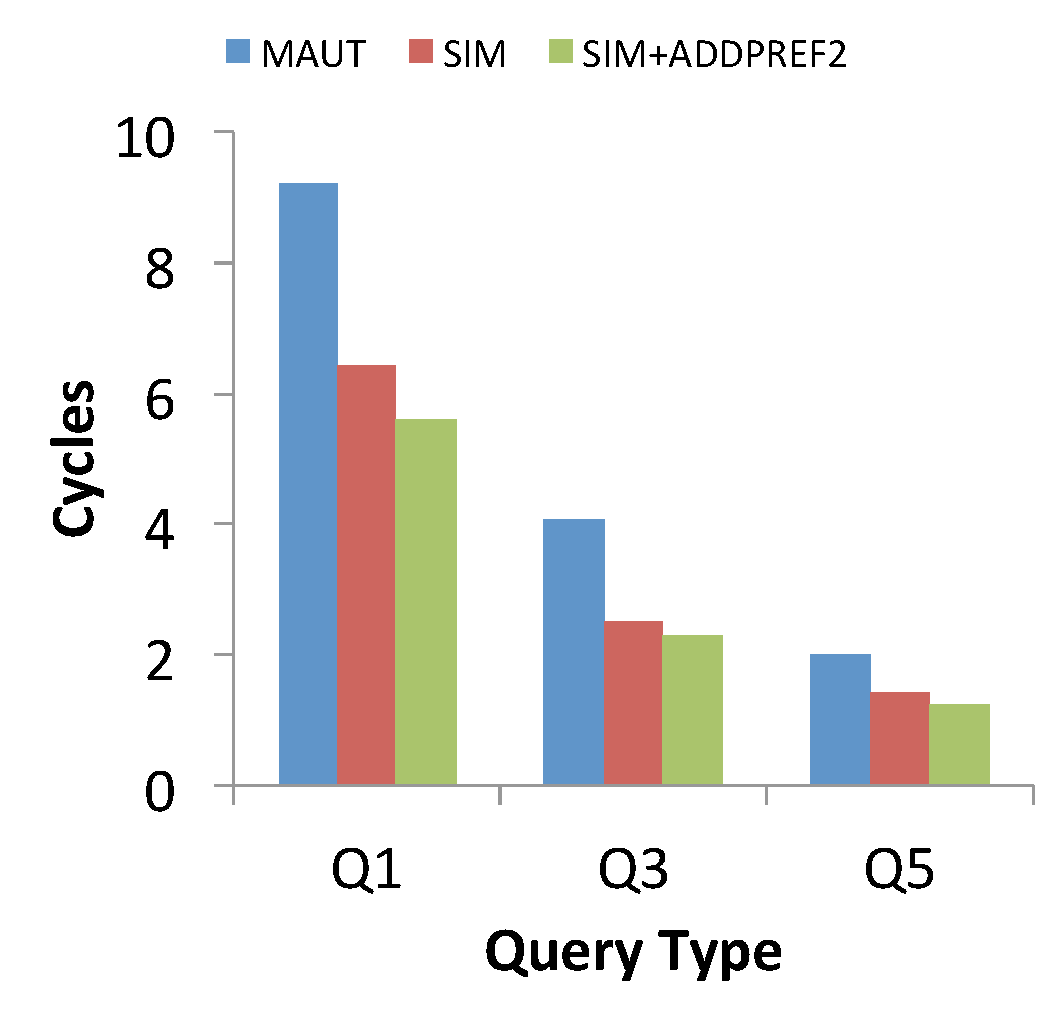
\includegraphics[width=1\linewidth]{figures-bharath/sim_camera_opt}
  \caption[]{Average number of interaction cycles on Camera dataset - optimal user model}
  \label{fig:sim_camera_opt}
\end{minipage}%
\;\;\;\;\;\;
\begin{minipage}{.45\textwidth}
  \centering
  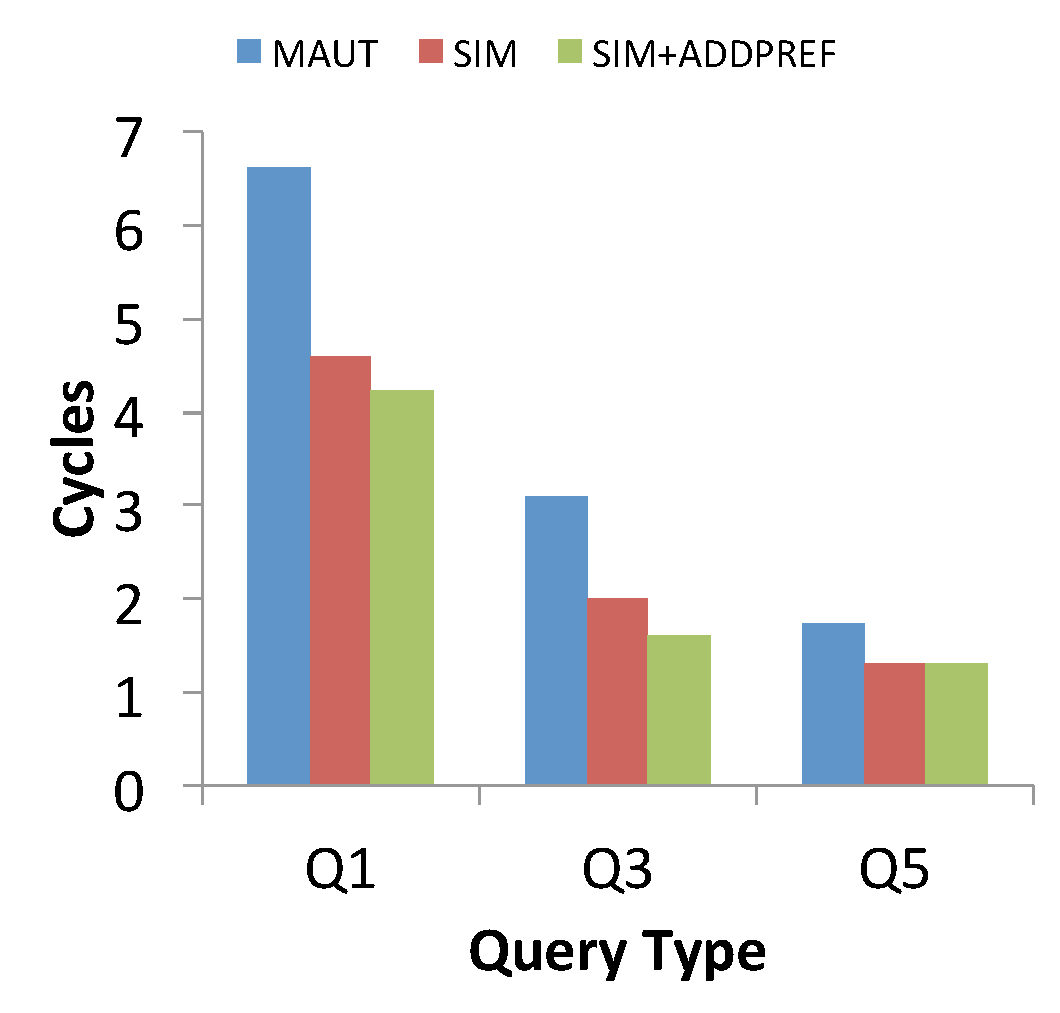
\includegraphics[width=1\linewidth]{figures-bharath/sim_pc_opt}
  \caption[]{Average number of interaction cycles on PC dataset - optimal user model}
  \label{fig:sim_pc_opt}
\end{minipage}
\end{figure}

\begin{figure}[h]
\centering
\begin{minipage}{.45\textwidth}
  \centering
  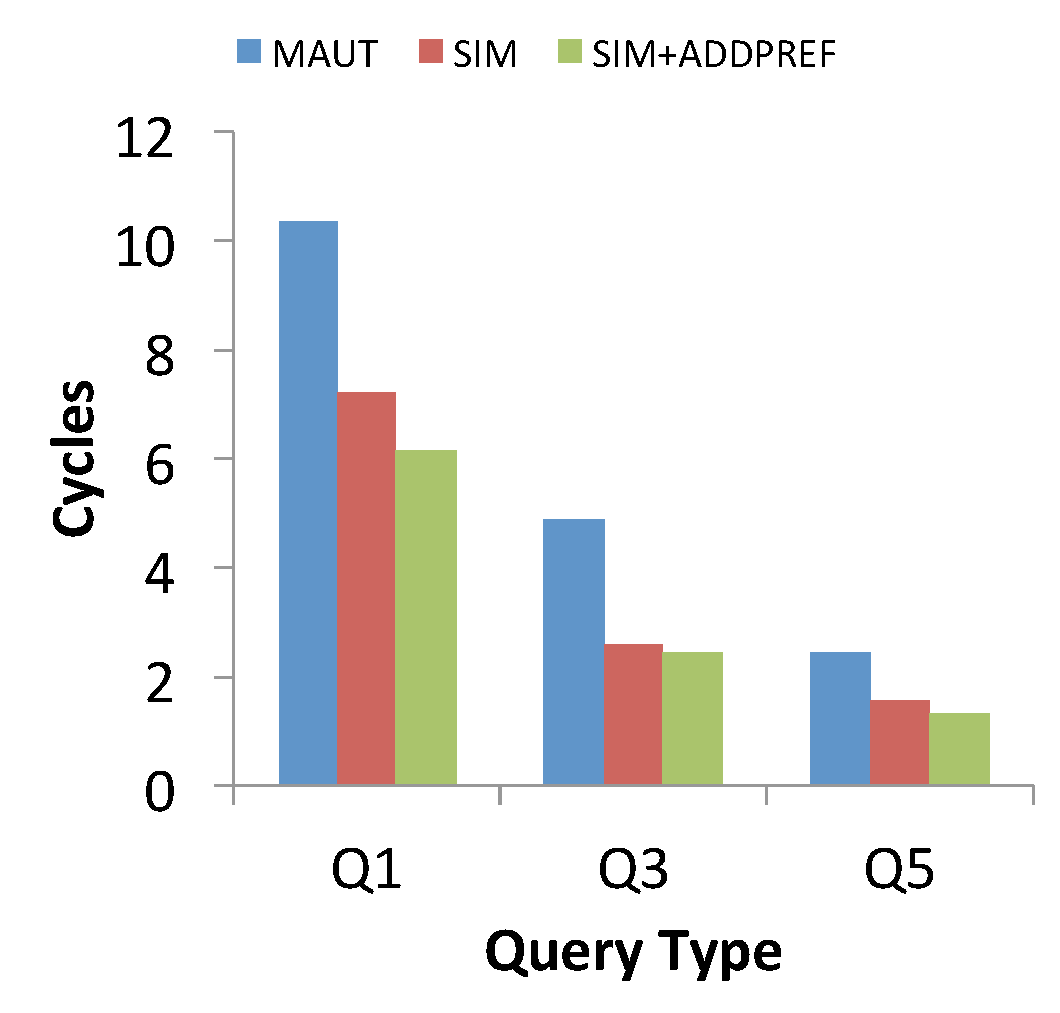
\includegraphics[width=1\linewidth]{figures-bharath/sim_camera_noisy}
  \caption[]{Average number of interaction cycles on Camera dataset - noisy framework}
  \label{fig:sim_camera_noisy}
\end{minipage}%
\;\;\;\;\;\;
\begin{minipage}{.45\textwidth}
  \centering
  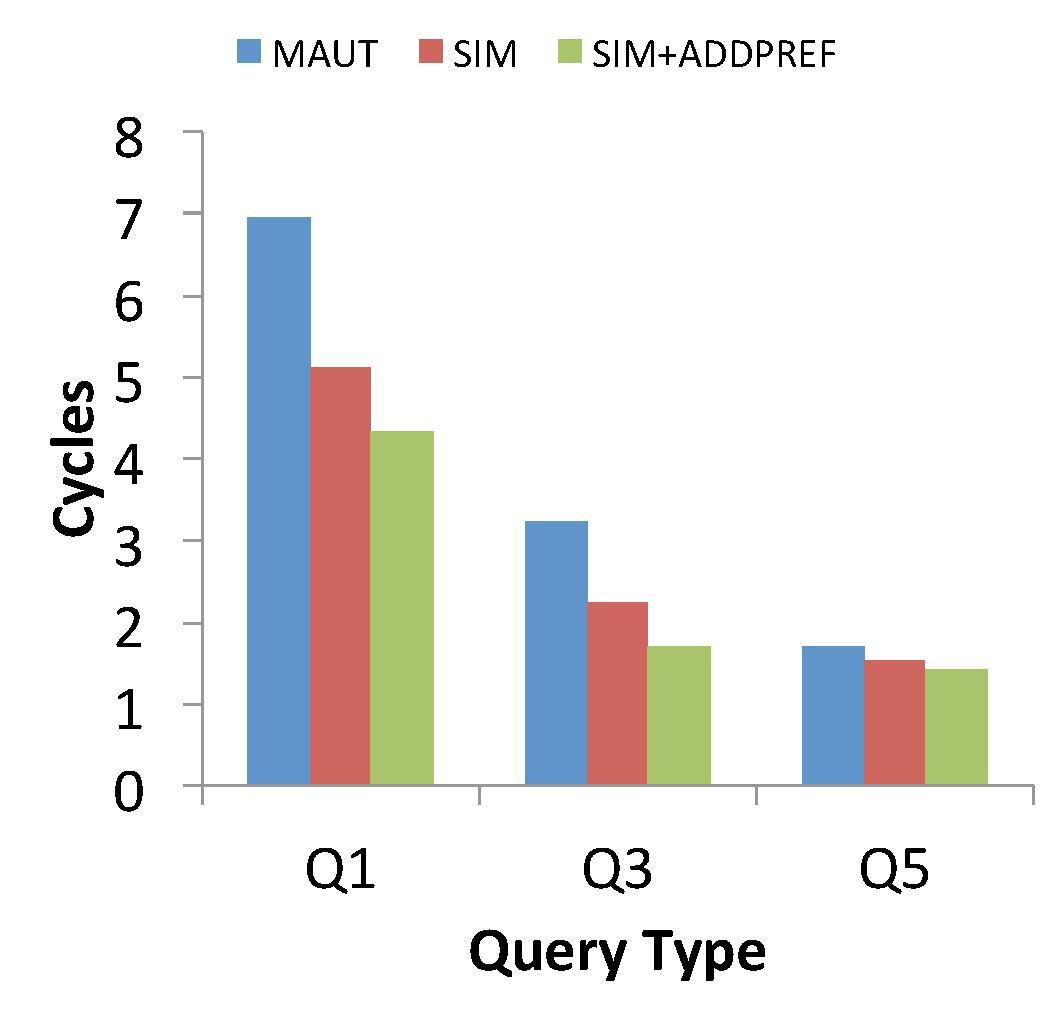
\includegraphics[width=1\linewidth]{figures-bharath/sim_pc_noisy}
  \caption[]{Average number of interaction cycles on PC dataset - noisy framework}
  \label{fig:sim_pc_noisy}
\end{minipage}
\end{figure}

\subsection{Algorithms that selectively update weights and value functions of attributes(SELWEIGHT and SELNOMINAL)}
The algorithm SELWEIGHT, described in Section \ref{sec:sel} that updates weights of numeric attributes by examining the critique patterns of selected product and also the $k-1$ rejected products.
SELNOMINAL, described in Section \ref{sec:selNominal} updates value functions by examining the nominal attribute values of the rejected $k-1$ products.
SELWEIGHT and SELNOMINAL take 7.65 and 7.08 cycles respectively for Camera dataset for the queries of type Q1 in an optimal framework.
When both the above algorithms are combined, the resulting algorithm performs better than both the individual algorithms.
The resulting algorithm takes only 6.78 cycles on an average to reach the target product.
MAUT takes 9.21 cycles on an average in this scenario.
%This means that SELWEIGHT and SELNOMINAL can guide the user through the product space very efficiently if the user is not very well aware of the domain.
%The superior performance of both SELWEIGHT and SELNOMINAL is maintained for Q3 as well as Q5 on both the datasets.
The number of interaction cycles taken by these two algorithms is shown in Figures \ref{fig:sel_camera_opt} to \ref{fig:sel_pc_noisy}.
The average improvement achieved by these algorithms in different scenarios is given in Table \ref{tab:summary}.

\begin{figure}[h]
\centering
\begin{minipage}{.45\textwidth}
  \centering
  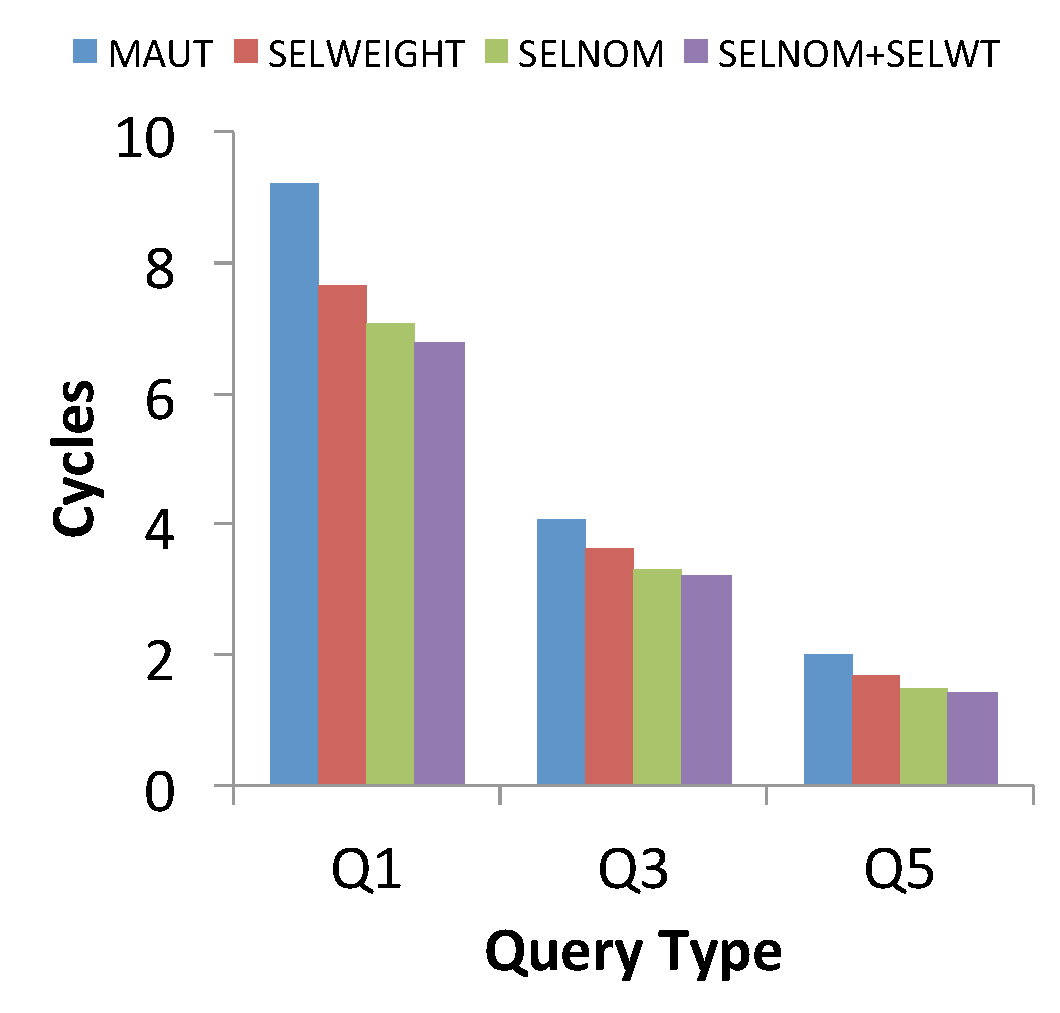
\includegraphics[width=1\linewidth]{figures-bharath/sel_camera_opt}
  \caption[]{Average number of interaction cycles on Camera dataset - optimal user model}
  \label{fig:sel_camera_opt}
\end{minipage}%
\;\;\;\;\;\;
\begin{minipage}{.45\textwidth}
  \centering
  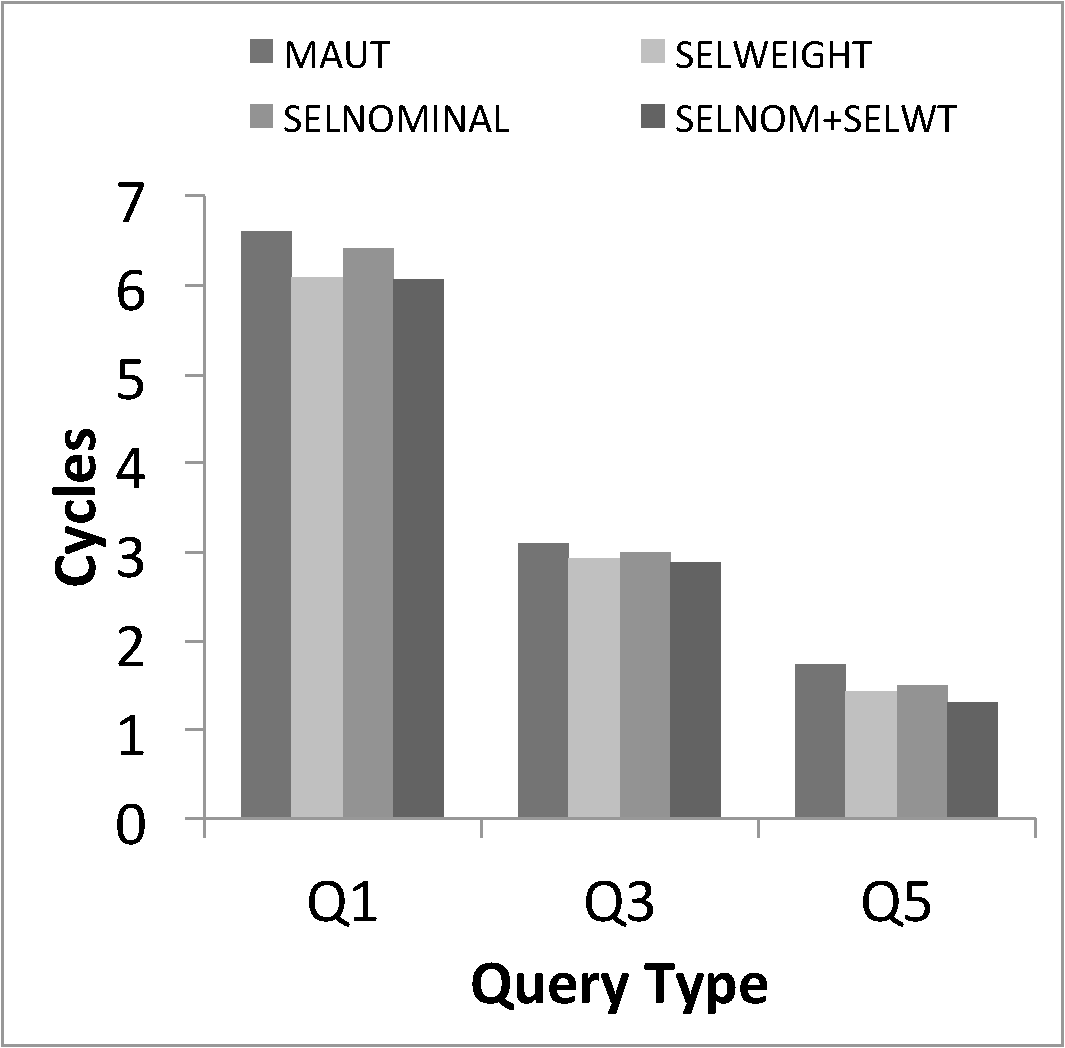
\includegraphics[width=1\linewidth]{figures-bharath/sel_pc_opt}
  \caption[]{Average number of interaction cycles on PC dataset - optimal user model}
  \label{fig:sel_pc_opt}
\end{minipage}
\end{figure}

\begin{figure}[h]
\centering
\begin{minipage}{.45\textwidth}
  \centering
  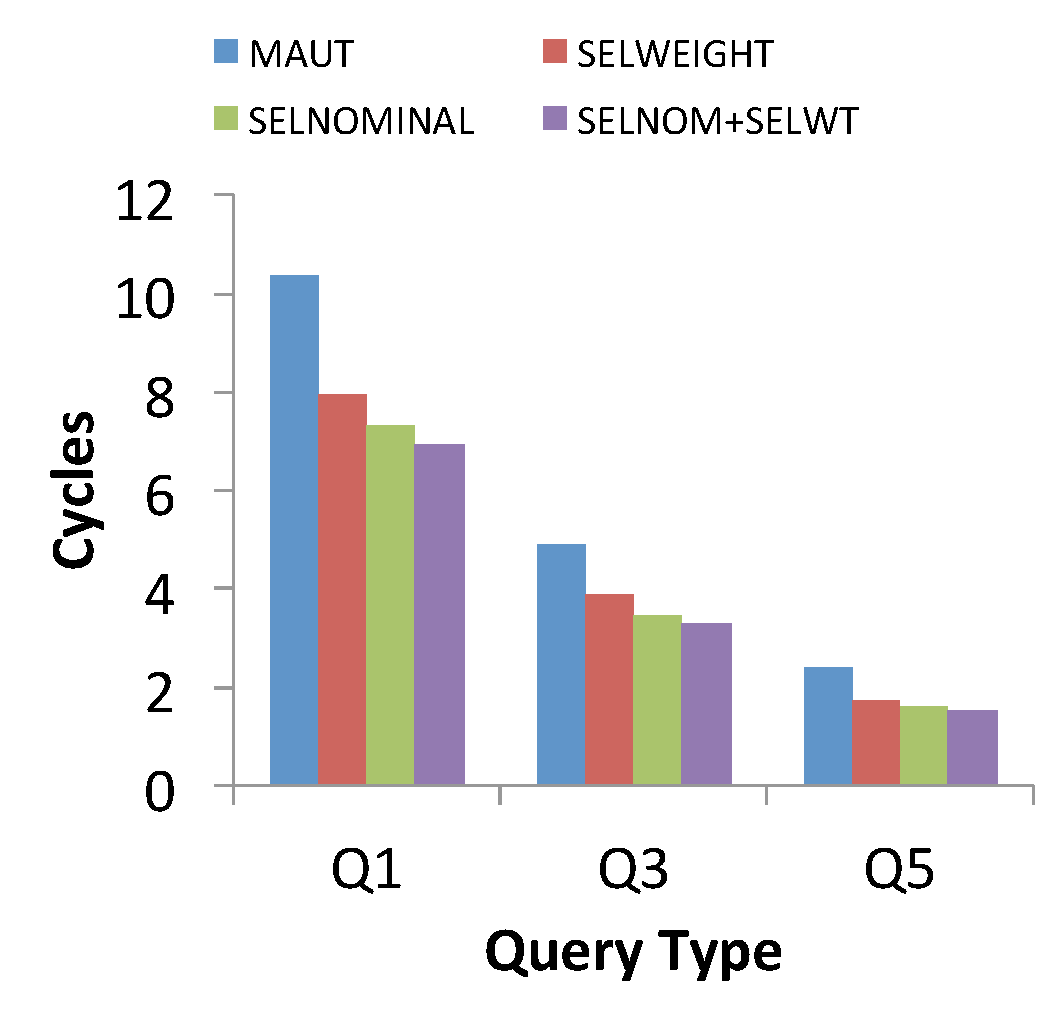
\includegraphics[width=1\linewidth]{figures-bharath/sel_camera_noisy}
  \caption[]{Average number of interaction cycles on Camera dataset - noisy framework}
  \label{fig:sel_camera_noisy}
\end{minipage}%
\;\;\;\;\;\;
\begin{minipage}{.45\textwidth}
  \centering
  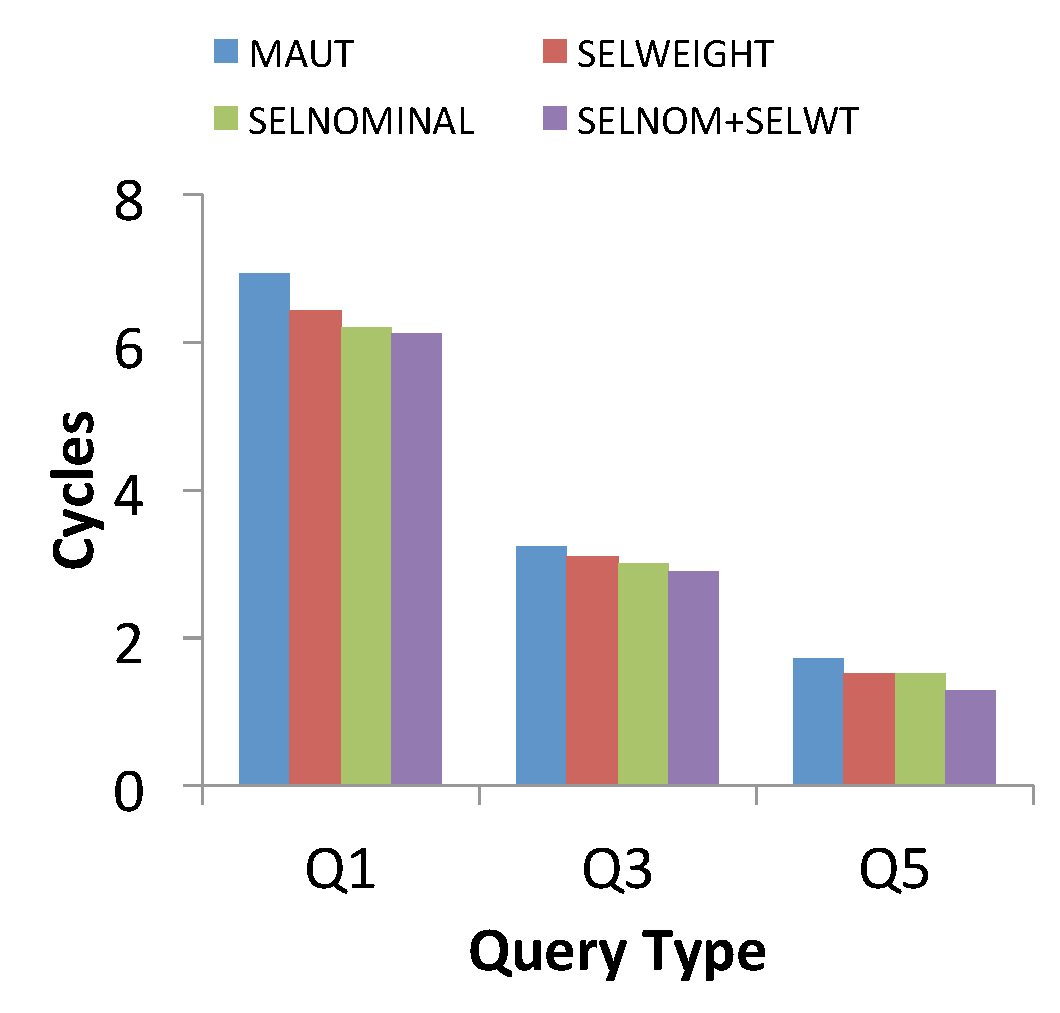
\includegraphics[width=1\linewidth]{figures-bharath/sel_pc_noisy}
  \caption[]{Average number of interaction cycles on PC dataset - noisy framework}
  \label{fig:sel_pc_noisy}
\end{minipage}
\end{figure}

\input{chap4_history}
\input{chap4_marketEq}
\input{chap4_additive}

%\chapter{Conclusions \& Future Work}
\label{chap:conclusions}
Our goal in this project was to improve the performance of MAUT based recommendation.
We have proposed several modifications to standard MAUT based recommendation algorithm in Sections \ref{sec:div} to \ref{sec:additive} which have led to significant performance improvements.
We first started by introducing diversity in the critique strings shown to the user.
The algorithm DIV displays maximally diverse critiques to the user in every cycle. 
Diverse critiques enable the user to navigate to different parts of the product space relatively quickly and hence, can potentially improve the performance of the algorithm.
%But, in an attempt to make the critiques diverse, the recommender will have to choose a few sub-optimal products as the top $K$ products in every cycle.
%So, there is also a risk of having prolonged sessions because of this, 
Offline experiments in Section \ref{sec:div_results} have shown that DIV enables the user to arrive at his target product much quicker than MAUT.
DIV2 varies the level of diversity in critique strings according to the extent to which the user's preferences were stabilized.
The performance of DIV2 is even better than DIV.

ADDPREF, described in Section \ref{sec:addTerm}, promotes products that have a critique pattern similar to the most recent product selected by the user.
ADDPREF2, an extension to ADDPREF, considers critique overlap of a product with all the products that have been selected so far.
Both these modifications lead to significant performance improvements.
SIM, described in Section \ref{sec:sim} displays products that are most similar to the user's query in the first cycle.
SIM is a very simple modification to the standard MAUT algorithm, but it results in a significant performance improvement.

SELWEIGHT described in Section \ref{sec:sel}, exploits the fact that a product/critique string was chosen over the remaining (k-1) rejected products and updates weights of numeric attributes accordingly. 
The default strategy in MAUT is to update weights of the attributes by a constant factor.
But SELWEIGHT updates weights of numeric attributes by different factors based on the critique patterns of the $k-1$ rejected products.
SELNOMINAL described in Section \ref{sec:selNominal} updates value function of a nominal attribute not just by looking at the attribute value of the selected product, but also by examining the nominal attribute $k-1$ rejected products.
Both SELWEIGHT and SELNOMINAL result in significant performance improvements.

The algorithm HIST, described in Section \ref{sec:hist}, computes the weighted average of the attribute values of products selected by the user in previous cycles and updates preference model according to these values.
INIT, described in Section \ref{sec:marketEq}, initializes the value functions of  nominal attributes of dominated products with higher values.
Finally, we describe an additive model, ADD, in Section \ref{sec:additive} for updating weights of numeric attributes in each cycle. 
Using additive model instead of the standard multiplicative model results in a significant performance improvement.


\section{Future Work}
In all the algorithms, we have used the simple weighted additive formula  (Equation \ref{eq:utility}) to estimate utilities of products assumes that the individual attributes are preferentially independent, which is not the case in real-world scenarios.
There could be additional terms in the utility function which correspond to the trade-offs between pairs of attributes.

We have also assumed very simple linear value functions for all the numeric attributes. 
%Using non-linear value functions could lead to improved perfomance.
%Exploring which kind of value functions 
Inferring better value functions automatically from user trials and the case base can lead to performance improvements and it is also an intersting problem to tackle.
%In Section \ref{sec:marketEq}, we have initialized only one attribute's value functions unequally. 
There is a lot of scope for improvements that can be done to the algorithm INIT described in Section \ref{sec:marketEq}.
The algorithm for exploiting the history of user selected products, HIST, described in Section \ref{sec:hist} is very simplistic as of now. 
Methods other than HIST can be explored to exploit the history of user selected products better.

%


\lipsum[1]
\begin{algorithm}
\begin{multicols}{2}
\begin{algorithmic}[1]
  \SetKwInOut{Input}{input}\SetKwInOut{Output}{output}
  \DontPrintSemicolon
  %\Input{$PM$, $IS$}

  $R \gets \{\}$\\
  $CB' \gets IS$\\
  \For{each attribute $x_i$ }{
      $ref[x_i] = 0$;\\
      $ws = 0$;\\
      \For{each product p $\in$ refL }{
          $ref[x_i] +=  hw_i \times p[x_i] $;\\
          $ws += hw_i$;\\
      }
      $ref[x_i] = ref[x_i]/ws$; \\
  }
  \For{each attribute $x_i$ in ref }{
      $[pv_i, pw_i] \leftarrow PM on x_i$;\\
      \If {$V(x_i) \geq pv_i$} {
          $pw_i' = pw_i \times \beta $;\\
      }
      \Else {
          $pw_i' = pw_i / \beta $;\\
      }
      $PM' \leftarrow [V(x_i), pw_i']$;\\
  }
  \Return $PM$;\\
  \caption{genAlgorithm}
  \label{algo:genAlgorithm}
\end{algorithmic}
\end{multicols}
\end{algorithm}
\lipsum[2]

% Appendices.
%\appendix

%\chapter{An Alternate Approach to Find Continuous Homomorphisms}
\label{chap:alt-hom-approaches}

In this appendix, we describe a technique we attempted to find
continuous homomorphisms. We did not continue, as the approach soon
became intractable.

\section{Modelling the State Space with a Gaussian Process}

We would like to unify our representation of continuous MDPs, using
Gaussian Processes (GP) as standard model; GPs can be easily learnt from
trajectories through the state space, and also model the stochasticity
of the world dynamics. A major limitation of using a Gaussian process to
model action behaviours is uni-modality; only actions which move the
agent in one direction, with noise, can be modelled. This limitation
could be overcome using a mixture of Gaussian processes, but that is out
of the scope of this thesis.

Consider a state space $S$. Let us assume that $S$ is a manifold, with
a mapping into $\Re^n$, $\xi$. For each point $x \in \Re^n$, there is an
associated {\em vector of Gaussian processes}, $\vec{a}$, representing
the behaviour of the actions. The transition dynamics can be described
by the following equation, $$T(s,a,s') = \frac{1}{Z} \exp( (\xi(s')
- m_a(\xi(s)))^T K^{-1}_a(\xi(s)) (\xi(s') - m_a(\xi(s)))),$$ where $m$
and $K$, are the mean and covariance of the Gaussian process. Continuous
actions can also be handled, using $m(\xi(s),\xi(a))$ and
$K^{-1}(\xi(s), \xi(a))$ in place of the respective subscripted
versions.

For the sake of notational convenience, we'll take $S = \Re^n$ in the
sequel. The results we present can be applied to the general continuous
state space through $\xi$.

\begin{figure}[h]
\centering
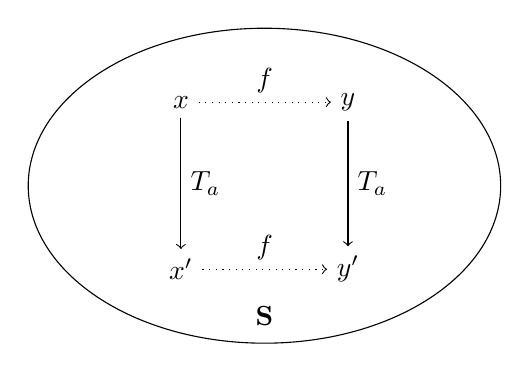
\begin{tikzpicture}
\usetikzlibrary{calc}

% Draw state spaces as rectangles
\draw (0,0) ellipse (3 and 2);
% Draw state space labels
\node at (0,-1.65) {$\mathbf{S}$};

% Xs
\node (x1) at ($(0,0) - (-45:1.5)$) {$x$};
\node (x2) at ($(0,0) - (45:1.5)$) {$x'$};
\draw[->] (x1) to node[auto]{$T_a$}  (x2);

% Ys
\node (y1) at ($(0,0) + (45:1.5)$) {$y$};
\node (y2) at ($(0,0) + (-45:1.5)$) {$y'$};
\draw[->] (y1) to node[auto]{$T_a$}  (y2);

% Map
\draw[->,dotted] (x1) to node[auto]{$f$} (y1);
\draw[->,dotted] (x2) to node[auto]{$f$} (y2);

\end{tikzpicture}
\caption{Bijective Automorphisms}
\label{fig:mdp-hom}
\end{figure}

Now, stating our problem in this framework, we would like to find
bijective automorphisms $f : S \to S$ that preserve the behaviour of the
transition dynamics described by $T_a$ for all actions $a \in \actions$.
At a high level, the diagram \autoref{fig:mdp-hom} describes what we
hope to achieve. Mathematically,
\begin{eqnarray*}
T_a(f(s),f(s')) -  T_a(s,s') &=& 0 \\
\frac{1}{|2\pi K_a(f(s))|} \exp((f(s') - m_a(f(s)))^T K^{-1}_a(f(s)) (f(s') - m_a(f(s)))) &-& \\
 \frac{1}{|2\pi K_a(s)|} \exp((s' - m_a(s))^T K^{-1}_a(s) (s' - m_a(s))) &=& 0.
\end{eqnarray*}

Aside from being in general intractable to solve, the above definition
is too strict for any practical domain. We will now explore two
relaxations that will let us find approximate homomorphisms.

\section{Bayesian Approach}
\label{sec:alt-hom-approaches:bayesian}
In this section, we will consider a Bayesian approach wherein the
mapping $f$ is itself a Gaussian process, $$f(x,y) = \frac{1}{Z}\exp(
(y-n(x))^T L^{-1}(x) (y-n(x)) )$$. We know that the probability of $y$
transitioning to $y'$, given $x$ and $x'$ are the respective pre-images
of $y$ and $y'$, is $T_a(x,x')$; $P(y \to y' | x \to y, x' \to y') = P(x
\to x')$. Thus, we have,

\begin{eqnarray*}
P(y \to y') &=& \int \ud x \ud x' ~ P(y \to y'|x \to y, x' \to y') P(x \to y) P(x' \to y') \\
T_a(y,y') &=& \int \ud x \ud x' ~ T_a(x,x') f(x,y) f(x',y').
\end{eqnarray*}

In the approximate setting, we would like to minimise the KL divergence
between the left and right-hand sides.
\begin{eqnarray*}
  T_a(y,y') &\approx& \int \ud x f(x,y) \E_{x'}[ f(x',y') ].\\
  \mL(y) &=& \E_{y'} [ \log T_a(y,y') - \log \int \ud x f(x,y) \E_{x'}[ f(x',y') ] ].
\end{eqnarray*}

If $\int \ud x f(x,y) = 1$, then we can apply Jensen's inequality to get,
\begin{eqnarray*}
  \mL(y) &\ge& \E_{y'} [ \log T_a(y,y') - \int \ud x f(x,y) \E_{x'}[ \log f(x',y') ] ].
\end{eqnarray*}

Note that $\log f(x',y')$ contains terms of complexity at most $\exp(x^T
A x + b^T x + c)$, which can be evaluated by Gaussian integral.

\begin{note}
  We can also take,
  \begin{eqnarray*}
    \mL(y) &\ge& [ \log T_a(y,y') - \int \ud x f(x,y) \E_{x'}[ \log \E_{y'}[ f(x',y') ] ] ].
  \end{eqnarray*}

  Note that $\E_{y'}$ here is over a {\em different distribution},
  namely $T_a(y,y')$ than $f(x',y')$, and hence not equal to $1$.
\end{note}

To proceed in this direction, we need a prior on $P(x)$, which is hard to
define. More importantly, an implict condition is that $\int \ud x P(x)
f(x,y) = 1$. This involves integrating over the mean function of
a Gaussian process; using the typical Gaussian kernel, the form of the
integrand is $e^{e^{x}}$, which is intractable. 



\begin{singlespace}
  \nocite{*}
%  \bibliography{thesis}
\end{singlespace}

\end{document}
